\documentclass[a4paper]{article}
\usepackage[a4paper,margin=0.75in]{geometry}
\usepackage[UTF8]{ctex}
%\usepackage[unicode={true}]{hyperref}
%\usepackage{amsthm}
\usepackage{amsmath}
\usepackage{graphicx} % Allows including images
\usepackage{subfigure}
%\usepackage{array}
\usepackage{indentfirst}
\usepackage{caption}
%\usepackage{cases}
%\usepackage{tikz}
%\usepackage[all,pdf]{xy}
%\usepackage{graph icx}
\usepackage{boondox-cal}
\usepackage{cancel}
%\usepackage[ruled,vlined]{algorithm2e}
%\usepackage[noend]{algpseudocode}
%\usepackage{algorithmicx}

\usepackage{booktabs}
%\renewcommand{\contentsname}{目录}

\usepackage{eucal}
\usepackage{mathrsfs}
\usepackage{algorithm}
\usepackage{algorithmic}

%---------------------------------------------------------------------------------------------------
% self-definition file
% created by Cui Zhen, 2014.02.05

%% ////////////////////////////////////////
%% useful package
\usepackage{amsthm}%Cui Zhen
\usepackage{amssymb}
\usepackage{cases}%Cui Zhen
\usepackage{bm}%Cui Zhen
\usepackage{algorithm}%Cui Zhen
\usepackage{algorithmic}%Cui Zhen
\usepackage{cases}%Cui Zhen
\usepackage{subfigure}%%cuizhen
\usepackage{multirow}%%cuizhen
\usepackage{xcolor} %% cuizhen
\usepackage{enumerate}%% cuizhen
\usepackage{etoolbox}%% cuizhen
\usepackage{boxedminipage} %% cuizhen
\usepackage{booktabs} %% cuizhen
%\usepackage[T1]{fontenc}
%% >> Define letters ========= begin ==========Cui Zhen===============
% need {etoolbox}
\DeclareMathOperator*{\argmin}{arg\,min}
\DeclareMathOperator*{\argmax}{arg\,max}
\newcommand{\MyMapTemplatePrefix}[4]{\expandafter#1\csname#3#4\endcsname{#2{#4}}}
\newcommand{\MyMapTemplatePrefixNew}[5]{\expandafter#1\csname#4#5\endcsname{#2{#3{#5}}}}
% bold upper letters: matrices or vectors = \A
\forcsvlist{\MyMapTemplatePrefix {\def} {\mathbf} {}} {A,B,C,D,E,F,G,H,I,J,K,L,M,N,O,P,Q,R,S,T,U,V,W,X,Y,Z}
% bold lower letters: matrices or vectors = \a\1\0
\forcsvlist{\MyMapTemplatePrefix {\def} {\mathbf} {}} {a,b,c,d,e,f,g,h,i,j,k,l,m,n,o,p,q,r,s,t,u,v,w,x,y,z,1,0}
% upper letters: \widetilde = \wt
\forcsvlist{\MyMapTemplatePrefix {\def} {\widetilde} {wt}} {A,B,C,D,E,F,G,H,I,J,K,L,M,N,O,P,Q,R,S,T,U,V,W,X,Y,Z}
% lower letters: \widetilde = \wt
\forcsvlist{\MyMapTemplatePrefix {\def} {\widetilde} {wt}} {a,b,c,d,e,f,g,h,i,j,k,l,m,n,o,p,q,r,s,t,u,v,w,x,y,z} % r
% upper letters: \widetilde\mathbf = \tb
\forcsvlist{\MyMapTemplatePrefixNew {\def} {\widetilde}{\mathbf} {tb}} {A,B,C,D,E,F,G,H,I,J,K,L,M,N,O,P,Q,R,S,T,U,V,W,X,Y,Z}
% lower letters: \widetilde\mathbf = \tb
\forcsvlist{\MyMapTemplatePrefixNew {\def} {\widetilde}{\mathbf} {tb}} {a,b,c,d,e,f,g,h,i,j,k,l,m,n,o,p,q,r,s,t,u,v,w,x,y,z}
% upper letters: \widehat = \wh
\forcsvlist{\MyMapTemplatePrefix {\def} {\widehat} {wh}} {A,B,C,D,E,F,G,H,I,J,K,L,M,N,O,P,Q,R,S,T,U,V,W,X,Y,Z}
% lower letters: \widehat = \wh
\forcsvlist{\MyMapTemplatePrefix {\def} {\widehat} {wh}} {a,b,c,d,e,f,g,h,i,j,k,l,m,n,o,p,q,r,s,t,u,v,w,x,y,z}
% upper letters: \widehat\mathbf = \hb
\forcsvlist{\MyMapTemplatePrefixNew {\def} {\widehat}{\mathbf} {hb}} {A,B,C,D,E,F,G,H,I,J,K,L,M,N,O,P,Q,R,S,T,U,V,W,X,Y,Z}
% lower letters: \widehat\mathbf = \hb
\forcsvlist{\MyMapTemplatePrefixNew {\def} {\widehat}{\mathbf} {hb}} {a,b,c,d,e,f,g,h,i,j,k,l,m,n,o,p,q,r,s,t,u,v,w,x,y,z}
% upper letters: \mathcal{G} = \mcG
\forcsvlist{\MyMapTemplatePrefix {\def} {\mathcal}{mc}} {A,B,C,D,E,F,G,H,I,J,K,L,M,N,O,P,Q,R,S,T,U,V,W,X,Y,Z}
% upper letters: \mathbb{G} = \mbG
\forcsvlist{\MyMapTemplatePrefix {\def} {\mathbb} {mb}} {A,B,C,D,E,F,G,H,I,J,K,L,M,N,O,P,Q,R,S,T,U,V,W,X,Y,Z}
% math operator
\forcsvlist{\MyMapTemplatePrefix {\DeclareMathOperator} {} {} } {tr,diag,sgn}
% others letters
\def\tp{^\intercal} \def\st{\text{s.t.~}}
\def\ie{\emph{i.e.}} \def\etal{\emph{et al.}}
\def\ptl{\partial~} \def\eg{\emph{e.g.}}
\def\phitb{\widetilde{\phi}}
\def\vs{\emph{vs. }}
%% new orders
\newcommand{\fix}{\marginpar{FIX}}
\newcommand{\new}{\marginpar{NEW}}
\newtheorem{thm}{Theorem}[section]
\newtheorem{defn}[thm]{Definition}
\newtheorem{prop}{Proposition}
\newcommand{\tabincell}[2]{\begin{tabular}{@{}#1@{}}#2\end{tabular}}%%
\renewcommand{\algorithmicrequire}{\textbf{Input:}}
\renewcommand{\algorithmicensure}{\textbf{Output:}}
\newcommand{\tabnote}[1]{\par\medskip\parbox{\textwidth}{#1}}
\hyphenation{all resp images image matrix sparse SFRD STFRD PMML its appearance transform}
\allowdisplaybreaks[4]
%---------------------------------------------------------------------------------------------------



\begin{document}

\setcounter{section}{0}

%---------------------------------------------------------------------------------------------------
\clearpage
\section{潜在的线性模型}
\subsection{因子分析-Factor analysis}

混合模型的一个问题是,它们仅使用单个潜在变量来生成观测值。特别是,每次观察只能来自K个原型中的一个。可以将混合模型视为使用K个隐藏二进制变量,表示集群标识的一个热编码。但由于这些变量相互排斥,模型的代表性仍然有限。 

另一种方法是使用实值潜变量向量,$\z_i\in\mathbb{R}^L$。使用前最简单的是高斯函数(稍后我们将考虑其他选择):
\begin{equation}
	p(\z_i)=\mathcal{N}(\z_i\vert\boldsymbol{\mu}_0,\textstyle\sum\nolimits_{0})\tag{12.1}
\end{equation}
如果观察也是连续的,那么$\x_i\in\mathbb{R}^D$,我们可以使用高斯函数表示可能性。与线性回归一样,我们将假设平均值是(隐藏)输入的线性函数,从而产生 :
\begin{equation}
	p(\x_i\vert\z_i,\theta)=\mathcal{N}(\W\z_i+\boldsymbol{\mu},\boldsymbol{\varPsi})\tag{12.2}
\end{equation}

其中,$\W$是$D\times L$矩阵,称为因子加载矩阵,$\boldsymbol{\varPsi}$是$D\times D$协方差矩阵。我们将$\boldsymbol{\varPsi}$视为对角,因为模型的整个要点是“强制”$\z_i$解释相关性,而不是“烘焙”到观测值的协方差。这种整体模型称为因子分析或FA。$\boldsymbol{\varPsi}=\sigma^2\I$的特殊情况称为概率主成分分析或PPCA。这个名字的原因稍后将变得明显。生成过程,其中$L=1,D=2$,$\boldsymbol{\varPsi}$是对角的,如图12.1所示。我们取一个各向同性高斯“喷雾罐”,沿$\w z_i+\mu$定义的1d线滑动。这会在2d中产生一个延迟(因此相关)高斯。 

\subsubsection{FA是MVN的低秩参数化}

FA可以被认为是一种使用少量参数在$\x$上指定关节密度模型的方法。要看到这一点,请注意,从等式4.126中,诱导边际分布$p(\x_i\vert\theta)$是高斯分布: 
\begin{align}
	p(\x_i\vert\theta)&=\int\mathcal{N}(\x_i\vert\W\z_i+\boldsymbol{\mu},\boldsymbol{\varPsi})\mathcal{N}(\z_i\vert\boldsymbol{\mu}_0,\textstyle\sum\nolimits_{0})d\z_i\tag{12.3}\\
	&=\mathcal{N}(\x_i\vert\W\boldsymbol{\mu}_0+\boldsymbol{\mu},\boldsymbol{\varPsi}+\W\textstyle\sum\nolimits_{0}\W^T)\tag{12.4}
\end{align}

\begin{figure}[h]
	\centering
	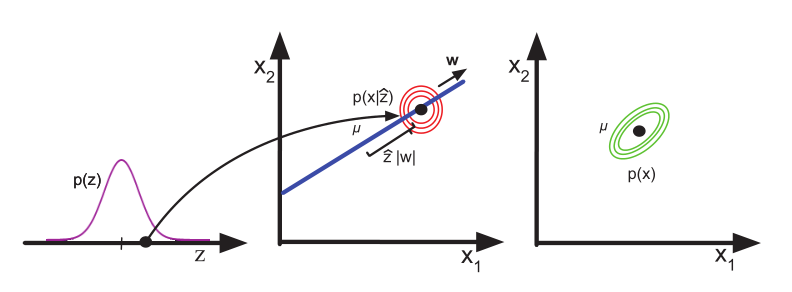
\includegraphics[width=1\linewidth]{fig/figure1}
	\caption*{图12.1: PPCA生成过程的图示,其中L=1个潜在维度生成D=2个观察维度。基于(Bishop 2006b)的图12.9。}
\end{figure}

\clearpage
由此我们可以看出,我们可以在不损失通用性的情况下设置$\boldsymbol{\mu}_0=0$,因为我们总是可以将$\W\boldsymbol{\mu}_0$吸收到$\boldsymbol{\mu}$中。类似地,我们可以设置$\sum\nolimits_{0}=\I$而不丧失通用性,因为我们可以通过定义新的权重矩阵$\tbW=\W\sum\nolimits_{0}^{-1/2}$来“模拟”相关实验,然后我们发现: 

\begin{equation}
cov[\x\vert\boldsymbol{\theta}]=\tbW^T+\mathbb{E}[\boldsymbol{\epsilon}\boldsymbol{\epsilon}^T]=(\W\textstyle\sum\nolimits_{0}^{-1/2})\sum\nolimits_{0}(\W\textstyle\sum\nolimits_{0}^{-1/2})^T+\boldsymbol{\varPsi}=\W\W^T+\boldsymbol{\varPsi}\tag{12.5}
\end{equation}

因此,我们看到FA使用低秩分解近似可见向量的协方差矩阵:
\begin{equation}
\C\triangleq cov[\x]=\W\W^T+\boldsymbol{\varPsi}
\tag{12.6}
\end{equation}

这仅使用O(LD)参数,这允许在具有$O(D^2)$参数的全协方差高斯和具有O(D)参数的对角协方差之间进行灵活的折衷。注意,如果我们不将$\boldsymbol{\varPsi}$限制为对角,我们可以很容易地将$\boldsymbol{\varPsi}$设置为全协方差矩阵;然后我们可以设置$\W=0$,在这种情况下,不需要潜在因素。

\subsubsection{潜在因素推断}
虽然FA可以被认为只是定义$\x$上密度的一种方法,但它经常被使用,因为我们希望潜在因子$\z$将揭示数据的有趣之处。为此,我们需要计算潜在因素的后验值。我们可以使用高斯的贝叶斯规则来给出:


\begin{align}
p(\z_i\vert\x_i,\boldsymbol{\theta})&=\mathcal{N}(\z_i\vert\m_i,\textstyle\sum\nolimits_{i})\tag{12.7}\\
\textstyle\sum\nolimits_{i}&\triangleq (\textstyle\sum\nolimits_{0}^{-1}+\W^T\boldsymbol{\varPsi}^{-1}\W)^{-1}\tag{12.8}\\
\m_i&\triangleq \textstyle\sum\nolimits_{i}(\W^T\boldsymbol{\varPsi}^{-1}(\x_i-\boldsymbol{\mu})+\textstyle\sum\nolimits_{0}^{-1}\boldsymbol{\mu}_0)\tag{12.9}
\end{align}

注意,在FA模型中,$\sum\nolimits_{i}$实际上独立于i,因此我们可以用$\sum$表示它。计算该矩阵需要$O(L^3+L^2D)$时间,计算每个$\m_i=\mathbb{E}[\z_i\vert\x_i,\boldsymbol{\theta}]$需要$O(L^2+LD)$时间。$\m_i$有时被称为潜在分数或潜在因子。 

\begin{figure}[h]
	\centering
	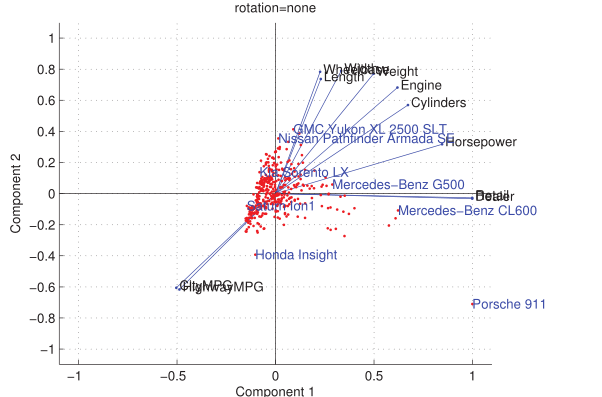
\includegraphics[width=1\linewidth]{fig/figure2}
	\caption*{图12.2: 基于因子分析的2004年cars数据的2D投影。蓝色文字是与某些选定点对应的汽车名称。图由faBiplotDemo生成。 }
\end{figure}

让我们举一个简单的例子,基于(Shalizi 2009)。我们考虑了一个由$D=11$变量和$N=387$个案例组成的数据集,这些案例描述了汽车的各个方面,例如发动机尺寸、气缸数量、每加仑英里数(MPG)、价格等。我们首先拟合了一个$L=2$维模型。我们可以将$\m_i$分数绘制为$\mathbb{R}^2$中的点,以可视化数据,如图12.2所示。 

为了更好地理解潜在因素的“意义”,我们可以将对应于每个特征维度的单位向量$\e_1=(1,0,...,0),\e_2=(0,1,...,0)$等投影到低维空间。这些在图12.2中显示为蓝线;这被称为双时隙。我们看到横轴代表价格,对应于标记为“经销商”和“零售”的功能,右侧是昂贵的汽车。纵轴表示燃油效率(以MPG为单位)与尺寸的关系:重型车辆效率较低,较高,而轻型车辆效率较高,较低。我们可以通过点击一些点来“验证”这种解释,并在训练集中找到最接近的样本,然后打印它们的名称,如图12.2所示。然而,正如我们在第12.1.3节中讨论的那样,一般来说,解释潜变量模型充满了困难。 

\subsubsection{不可辨识性}
就像混合模型一样,FA也是无法识别的。为了说明这一点,假设$\R$是一个任意正交旋转矩阵,满足$\R\R^T=\I$。让我们定义$\tbW=\W\R$。那么可能修正矩阵的函数与未修正矩阵的函数相同,因为:

\begin{align}
cov[\x]&=\tbW\mathbb{E}[\z\z^T]\tbW^T+\mathbb{E}[\boldsymbol{\epsilon}\boldsymbol{\epsilon}^T]\tag{12.10}\\
&=\W\R\R^T\W^T+\boldsymbol{\varPsi}=\W\W^T+\boldsymbol{\varPsi}\tag{12.11}
\end{align}

几何上,将$\W$乘以正交矩阵就像在生成$\x$之前旋转$\z$;但由于$\z$是从各向同性高斯中提取的,因此这对可能性没有影响。因此,我们无法唯一识别$\W$,因此也无法唯一识别潜在因素。 

为了确保唯一的解决方案,我们需要删除$L(L-1)/2$自由度,因为这是大小为$L \times L$
\footnote{要看到这一点,请注意$L-1$在R中的自由参数在第一列中(因为列向量必须归一化为单位长度),有$L-2$第二列中的2个自由参数(必须与第一列正交),依此类推。 }

的正交矩阵的总数,FA模型具有$D+LD-L(L-1)/2$自由参数(不包括平均值),其中第一项来自$\boldsymbol{\varPsi}$。显然,我们要求它小于或等于$D(D+1)/2$,这是无约束(但对称)协方差矩阵中的参数数。这给了我们一个关于L的上界,如下:

\begin{equation}
	L_{max}=\lfloor+0.5(1-\sqrt{1+8D})\rfloor\tag{12.12}
\end{equation}

例如,$D=6$意味着$L\leqslant3$.但我们通常从不选择这个上限,因为它会导致过度拟合(见第12.3节关于如何选择L的讨论)。 
不幸的是,即使我们设置$L<L_{max}$,我们仍然无法唯一识别参数,因为旋转模糊仍然存在。不可识别性不会影响模型的预测性能。然而,它确实会影响载荷矩阵,从而影响潜在因素的解释。由于因子分析通常用于揭示数据中的结构,因此需要解决这个问题。以下是一些常用的解决方案: 

\begin{itemize}
\item \textbf{强迫$\W$正交}:可能是可识别性问题的最干净的解决方案是强迫$\W$正交,并通过减少相应潜在因子的方差来对列排序。这是主成分分析采用的方法,我们将在第12.2节中讨论。结果不一定更容易解释,但至少是独特的。 
\item \textbf{$\W$强制为下三角形}:将$\W$强制为下三角形是实现可识别性的一种方法,这在贝叶斯社区(例如,(Lopes and West 2004))中很流行,其目的是确保第一个可见特征仅由第一个潜在因子生成,第二个可见特征仅由前两个潜在因子生成,等等。例如,如果$L=3,D=4$,则相应的因子载荷矩阵由下式给出: 
\[ \mathbf{W} = \left(
\begin{array}{cccc}
w_{11} & 0  & 0\\
w_{21} & w_{22}  & 0\\
w_{31} & w_{32} &  w_{33}\\
w_{41} & w_{42} &  w_{43}\\ \tag{12.13}
\end{array} \right) \]

对于$j=1:L$,我们还要求$w_{jj}>0$。该约束矩阵中的参数总数为$D+DL-L(L-1)/2$,等于唯一可识别参数的数量。这种方法的缺点是,前L个可见变量被称为创始人变量,是影响解读的潜在因素,因此必须慎重选择。 
\end{itemize}



\begin{itemize}
\item \textbf{稀疏性促进权重先验 }:不是预先指定$\W$中的哪些条目为零,我们可以使用$\ell
_1$正则化(Zou等人,2006),ARD(Bishop 1999;Archambeau和Bach 2008),或spike和slab先验(Rattray等人,2009)。这称为稀疏因子分析。这并不一定能确保唯一的MAP估计,但它确实鼓励可解释的解决方案。见第13.8节。
\item \textbf{选择信息旋转矩阵}:有多种启发式方法试图找到旋转矩阵$\R$,旋转矩阵$\R$可用于修改$\W$(以及潜在因子),从而尝试增加可解释性,通常是通过鼓励它们(近似)稀疏。一种流行的方法是varimax(Kaiser 1958)。 
\item \textbf{对潜在因素使用非高斯预设值}:在第12.6节中,我们将讨论用非高斯分布代替$p(\z_i)$如何使我们有时能够唯一地识别$\W$以及潜在因素。这种技术被称为独立分量分析。 
\end{itemize}

\begin{figure}[h]
	\centering
	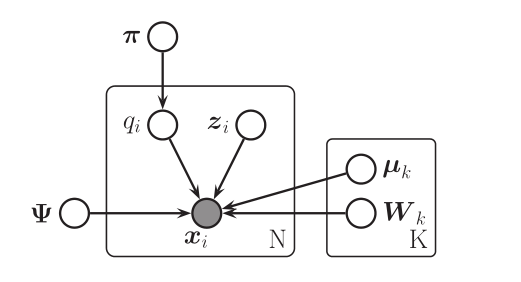
\includegraphics[width=1\linewidth]{fig/figure3}
	\caption*{图12.3: 混合因子分析仪作为DGM。 }
\end{figure}


\subsubsection{因素分析器的混合物}
FA模型假设数据存在于低维线性流形上。事实上,大多数数据最好用某种形式的低维曲线流形建模。我们可以用分段线性流形近似曲线流形。这表明了以下模型:让维数$L_k$的第k个线性子空间由$\W_k$表示,$k=1:\K$。假设我们有一个潜在指示符$q_i\in\{1,...,K\}$指定我们应该使用哪个子空间来生成数据。然后,我们从高斯先验中采样$\z_i$,并将其通过$\W_k$矩阵(其中$k=q_i$),然后添加噪声。更准确地说,模型如下: 
\begin{align}
p(\x_i\vert\z_i,q_i=k,\boldsymbol{\theta})&=\mathcal{N}(\x_i\vert\boldsymbol{\mu}_k+\W_k\z_i,\boldsymbol{\varPsi})\tag{12.14}\\
p(\z_i\vert\boldsymbol{\theta})&=\mathcal{N}(\z_i\vert\boldsymbol{0},\I)\tag{12.15}\\
p(q_i\vert\boldsymbol{\theta})&=Cat(q_i\vert\boldsymbol{\pi})\tag{12.16}
\end{align}


\begin{figure}[h]
	\centering
	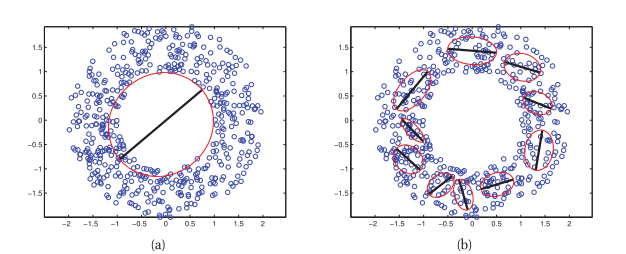
\includegraphics[width=1\linewidth]{fig/figure4}
	\caption*{图12.4: 拟合数据集的1d PPCA的混合物,$K = 1, 10$。图由mixPpcaDemoNetlab生成。 }
\end{figure}

这被称为\textbf{因子分析仪的混合物}(MFA)(Hinton等人,1997年)。CI假设如图12.3所示。

另一种考虑该模型的方法是将其视为高斯混合的低秩版本。特别是,该模型需要$O(KLD)$参数,而不是全协方差高斯混合所需的$O(KD^2)$参数。这可以减少过度装配。事实上,MFA是高维实值数据的良好通用密度模型。 
\subsubsection{因素分析模型的EM}
利用第4章的结果,可以直接推导出一种EM算法来拟合FA模型。只需再多做一点工作,我们就可以适应混合FA。下面我们陈述了没有证据的结果。推导见(Ghahramani和Hinton 1996a);然而,如果你想精通数学,自己推导这些方程是一个有用的练习。

为了获得单因素分析仪的结果,只需在以下等式中设置$r_{ic}=1$和$c=1$。在第12.2.5节中,我们将看到在拟合PPCA模型时产生的这些方程的进一步简化,结果将具有特别简单和优雅的解释。 

在E步骤中,我们用以下方法计算数据点$i$的集群$c$的后验责任。
\begin{equation}
	r_{ic}\triangleq p(q_i=c\vert\x_i,\boldsymbol{\theta}) \propto \pi_c\mathcal{N}(\x_i\vert\boldsymbol{\mu_c},\W_c\W_c^T+\boldsymbol{\varPsi})\tag{12.17}
\end{equation}

$\z_i$的条件后验值由以下公式得出:
\begin{align}
	p(\z_i\vert\x_i,q_i=c,\boldsymbol{\theta})  &=  \mathcal{N}(\z_i\vert\m_{ic},\textstyle\sum\nolimits_{ic})\tag{12.18}\\
	\textstyle\sum\nolimits_{ic}  &\triangleq  (\I_L+\W_c^T\boldsymbol{\varPsi}_c^{-1}\W_c)^{-1}\tag{12.19}\\
	\m_{ic}  &\triangleq  \textstyle\sum\nolimits_{ic}(\W_c^T\boldsymbol{\varPsi}_c^{-1}(\x_i-\boldsymbol{\mu}_c))\tag{12.20}
\end{align}

在M步骤中,最简单的是同时估计$\boldsymbol{\mu}_c$和$\W_c$,通过定义$\tbW_c=(\W_c,\boldsymbol{\mu}_c),\tbz=(\z,1)$,此外,定义:
\begin{align}
	\b_{ic}\  &\triangleq\  \mathbb{E}[\tbz\vert\x_i,q_i=c]=[\m_{ic};1]\tag{12.21}\\
	\C_{ic}\  &\triangleq\  \mathbb{E}[\tbz\tbz^T\vert\x_i,q_i=c]=\left(
	\begin{array}{cccc}
	\mathbb{E}[\z\z^T\vert\x_i,q_i=c] & \mathbb{E}[\z\vert\x_i,q_i=c] \\
	\mathbb{E}[\z\vert\x_i,q_i=c]^T & 1
	\end{array} \right)\tag{12.22}
\end{align}

然后M步骤如下:
\begin{align}
	\hat{\tilde{W}}_c\ &=\ \displaystyle \left[
\sum_{i}r_{ic}\x_i\b_{ic}^T\right]\displaystyle \left[
\sum_{i}r_{ic}\C_{ic}\right]^{-1}\tag{12.23}\\
	\hat{\boldsymbol{\varPsi}}\  &=\ \frac{1}{N}diag \left\{\sum_{i}r_{ic}\left (\x_i-\hat{\tilde{W}}_c\b_{ic}\right)\x_i^T\right\} \tag{12.24}\\
	\hat{\pi}_c\  &=\ \frac{1}{N}\sum_{i=1}^{N}r_{ic}\tag{12.25}
\end{align}

请注意,这些更新是针对“vanilla”EM的。基于ECM的该算法的更快版本如(Zhao和Yu 2008)所述。

\subsubsection{缺失数据的FA模型拟合 }

在许多应用程序中,例如协同过滤,我们会丢失数据。EM方法拟合FA/PPCA模型的一个优点是很容易扩展到这种情况。然而,如果有大量缺失数据,则过度拟合可能是一个问题。因此,进行MAP估计或使用贝叶斯推理很重要。详见(Ilin和Raiko 2010)。

\subsection{主成分分析(PCA) }

考虑FA模型,其中我们约束$\boldsymbol{\varPsi}=\sigma^2\I$,$\W$为正交。可以证明(Tipping和Bishop 1999),作为$\sigma^2\rightarrow 0$时,该模型简化为经典\textbf{(非概率)主成分分析(PCA)}(,也称为\textbf{arhunen-Loeve变换}。$\sigma^2>0$的版本称为\textbf{概率主成分分析(PPCA)}(Tipping和Bishop 1999),或\textbf{合理主成分分析}(Roweis 1997)。(从不同角度独立得出了一个等效结果,见(Moghaddam和Pentland 1995) 

为了理解这个结果,我们首先必须学习经典主成分分析。然后,我们将主成分分析连接到奇异值分解。最后我们再来讨论PPCA。 
\subsubsection{经典PCA:定理陈述 }

在下面的定理中总结了经典主成分分析(PCA)的\textbf{综合观点}。 

\newtheorem{mythm}{My Theorem}[subsection]
\begin{mythm}\label{thm:light}
	假设我们想要找到$L$线性基向量的正交集$\w_j\in\mathbb{R}^D$和相应的分数$\z_i\in\mathbb{R}^D$,使平均重建误差最小化,
\begin{equation}
	J(\W,\Z)=\frac{1}{N}\sum_{i=1}^{N}\parallel\x_i-\hat{\x_i}\parallel^2\tag{12.26}
\end{equation}
\end{mythm}

\begin{figure}[h]
	\centering
	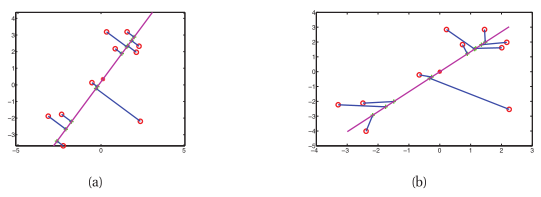
\includegraphics[width=1\linewidth]{fig/figure5}
	\caption*{图12.5 在D=2和L=1的情况下,PCA和PPCA的说明。圆圈是原始数据
		点,交叉点是重构的数据。红星是数据的平均值。(a) PCA。这些点被正交地
		投射到线上。图由pcaDemo2d生成。(b) PPCA。投影不再是正交的了。
		重构的数据向数据平均值缩减(红星)。基于(Nabney 2001)的图7.6。
		图由ppcaDemo2d生成。}
\end{figure}

其中$\hbx_i=\W\z_i$,受$\W$是正交的约束。等价地,我们可以将此目标写为: 
\begin{equation}
		J(\W,\Z)=\parallel\X-\W\Z^T\parallel_F^2\tag{12.27}
\end{equation}

其中$\Z$是一个$N \times L$矩阵,其中$\z_i$在其行中,$\parallel\A\parallel$是矩阵$\A$的\textbf{Frobenius范数},定义如下:

\begin{equation}
	\parallel\A\parallel_F \ =\  \sqrt{\sum_{i=1}^{m}\sum_{j=1}^{n}a_{ij}^2}\ =\ \sqrt{tr(\A^T\A)}\ =\ \parallel\A(:)\parallel_2 \tag{12.28}
\end{equation}

通过设置$\hat{\W}=\V_L$获得最优解,其中$\V_L$包含具有经验协方差矩阵最大特征值的L个特征向量$\hat{\textstyle \sum}=\frac{1}{N}\sum\nolimits_{i=1}^N\x_i\x_i^T$(为了符号简单起见,我们假设$\x_i$具有零均值。)此外,数据的最佳低维编码由$\hat{\z}_i=\W^T\x_i$给出,这是数据在特征向量跨越的列空间上的正交投影。

图12.5(a)中显示了$D=2$和$L=1$的示例。对角线是矢量$\w_1$;这被称为第一主分量或主方向。数据点$\x_i\in\mathbb{R}^2$正交投影到这条线上,得到$z_i\in\mathbb{R}$、 这是对数据的最佳一维近似。(稍后我们将讨论图12.5(b) 

一般来说,很难将高维数据可视化,但如果这些数据恰好是一组图像,就很容易做到。一组图像,就很容易做到这一点。图12.6显示了前三个主向量,重塑为图像,以及使用不同数量的基向量重建特定图像。(我们在第11.5节中讨论了如何选择$L$。) 

下面我们将表明,主方向是数据显示最大方差的方向。这意味着主成分分析可能仅仅因为测量尺度而被方差高的方向“误导”。图12.7(a)显示了一个示例,其中纵轴(重量)使用的范围比横轴(高度)大,导致线条看起来有些“不自然”。 因此,标准做法是首先标准化数据,或等效地使用相关矩阵而不是协方差矩阵。从图12.7(b)中可以明显看出这一点的好处。 

\begin{figure}[h]
	\centering
	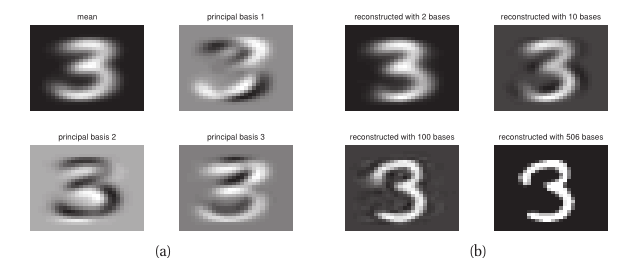
\includegraphics[width=1\linewidth]{fig/figure6}
	\caption*{图12.6:(a)基于数字3的25个图像(来自MNIST数据集)的平均值和前三个PC基向量(特征数字)。(b) 基于2、10、100和所有基向量重建图像。由pcaImageDemo生成的图。 }
\end{figure}

\clearpage
\begin{figure}[h]
	\centering
	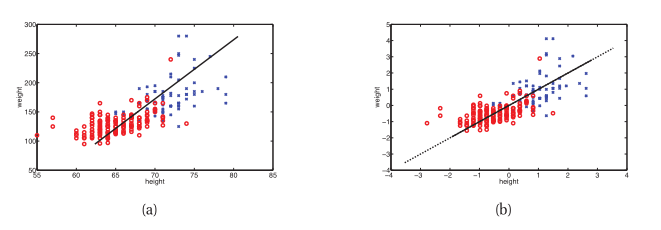
\includegraphics[width=1\linewidth]{fig/figure7}
	\caption*{图12.7: 标准化对应用于身高/体重数据集的主成分分析的影响。左:原始数据的主成分分析。右:标准化数据的主成分分析。pcaDemoHeightWeight生成的图。 }
\end{figure}

\subsubsection{证明* }

证明:我们使用$\w_j\ \in \ \mathbb{R}^D$表示第j个主方向,$\x_i\in\mathbb{R}^D$表示第i个高维观测,$\z_i\in\mathbb{R}^L$表示第i个低维表示,和$\tbz_j\in\mathbb{R}^N$表示$[z_{1j},...,z_{Nj}]$,它是所有低维向量的第j个分量。 

让我们从估计最佳1d解,$\w_1\in\mathbb{R}^D$,以及相应的投影点$\tbz_1\in\mathbb{R}^N$开始。我们将在后面找到其余的基数$\w_2,\w_3$等。重建误差由以下公式给出:

\begin{align}
	J(\w_1,\z_1)\ &=\ \frac{1}{N}\sum_{i=1}^{N}\parallel\x_i-z_{i1}\w_1\parallel^2\ =\ \frac{1}{N}\sum_{i=1}^{N}(\x_i-z_{i1}\w_1)^T(\x_i-z_{i1}\w_1)\tag{12.29}\\
	&=\ \frac{1}{N}\sum_{i=1}^{N}[\x_i^T\x_i-2z_{i1}\w_1^T\x_i+z_{i1}^2\w_1^T\w_1]\tag{12.30}\\
	&=\ \frac{1}{N}\sum_{i=1}^{N}[\x_i^T\x_i-2z_{i1}\w_1^T\x_i+z_{i1}^2]\tag{12.31}\\
\end{align}

由于$\w_1^T\w_1=1$(根据正交性假设)。取导数$wrt\ z_{i1}$并等于零,得到:
\begin{equation}
	\dfrac{\partial}{\partial z_{i1}}j(\w_1,\z_1)=\frac{1}{N}[-2\w_i^T\x_i+2z_{i1}]=0\Rightarrow z_{i1}=\w_1^T\x_i\tag{12.32}
\end{equation}

因此,通过将数据正交投影到第一主方向$\w_1$上获得最佳重建权重(见图12.5(a))。插回会得到:

\begin{equation}
	J(\w_1)\ =\ \frac{1}{N}\sum_{i=1}^{N}[\x_i^T\x_i-z_{i1}^2]\ =\ const-\frac{1}{N}\sum_{i=1}^{N}z_{i1}^2\tag{12.33}
\end{equation}

现在,投影坐标的方差由以下公式给出:
\begin{equation}
	var[\tbz_1]\ =\ \mathbb{E}[\tbz_1^2]\ -\ (\mathbb{E}[\tbz_1])^2\ =\ \frac{1}{N}\sum_{i=1}^{N}z_{i1}^2-0\tag{12.34}
\end{equation}

由于:
\begin{equation}
	\mathbb{E}[z_{i1}]\ =\ \mathbb{E}[\x_i^T\w_1]\ =\ \mathbb{E}[\x_i]^T\w_1\ =\ 0\tag{12.35}
\end{equation}

因为数据已经被居中了。由此我们可以看出,最小化重建误差相当于使投影数据的方差最大化,即:
\begin{equation}
	arg\ \min_{\w_1}\ J(\w_1)=arg\ \max_{\w_1}\ var[\tbz_1]  \tag{12.36}
\end{equation}

这就是为什么人们经常说主成分分析可以找到最大方差的方向。这称为PCA的\textbf{分析视图}。

预测数据的方差可以写成:
\begin{equation}
	\frac{1}{N}\sum_{i=1}^{N}z_{i1}^2\ =\ \frac{1}{N}\sum_{i=1}^{N}\w_1^T\textstyle{\hat\sum}\w_1\tag{12.37}
\end{equation}

其中$\textstyle\boldsymbol{\hat{\sum}}\ =\ \frac{1}{N}\sum_{i=1}^{N}\sum\nolimits_{i}\x_i\x_i^T$是经验协方差矩阵(如果数据标准化,则为相关矩阵)。 


我们可以通过让$||\w_1||\ \rightarrow\ \infty$使投影的方差最小化(从而最小化重建误差),因此我们施加约束$||\w_1|| =1$,代替最大化。

\begin{equation}
	\wtJ(\w_1)\ =\ \w_1^T\textstyle\boldsymbol{\hat{\sum}}\w_1\ +\ \lambda_1(\w_1^T\w_1-1)\tag{12.38}
\end{equation}


其中$\lambda_1$是拉格朗日乘子。取导数并等于零,我们有:

\begin{align}
	\dfrac{\partial}{\partial \w_1}\wtJ(\w_1)\ &=\ 2\textstyle\boldsymbol{\hat{\sum}}\w_1-2\lambda_1\w_1\ =\ 0\tag{12.39}\\
	\textstyle\boldsymbol{\hat{\sum}}\w_1\ &=\ \lambda_1\w_1\tag{12.40}
\end{align}

因此,方差最大化的方向是协方差矩阵的特征向量。左乘以$\w_1$(使用$\w_1^T\w_1=1$),我们发现投影数据的方差为:
 
\begin{equation}
	\w_1^T\textstyle\boldsymbol{\hat{\sum}}\w_1\ =\ \lambda_1\tag{12.41}
\end{equation}

由于我们想要最大化方差,我们选择对应于最大特征值的特征向量。
现在,让我们找到另一个方向$\w_2$,以进一步最小化重建误差,前提是$\w_1^T\w_2=0$和$\w_2^T\w_2=1$。错误是:

\begin{equation}
	J(\w_1,\z_1,\w_2,\z_2)=\frac{1}{N}\sum_{i=1}^{N}\parallel\x_i-z_{i1}\w_1-z_{i2}\w_2\parallel^2\tag{12.42}
\end{equation}

优化wrt $\w_1$和$\z_1$得到了与之前相同的解决方案。练习12.4要求你展示$\frac{\partial J}{\partial \z_2}=0$产生$z_{i2}=\w_2^T\x_i$。换句话说,通过投影到第二主方向来获得第二主编码。代入后得到的结果是:

\begin{equation}
	J(\w_2)\ =\ \frac{1}{n}\sum_{i=1}^{N}[\x_i^T\x_i-\w_1^T\x_i\x_i^T\w_1-\w_2^T\x_i\x_i^T\w_2]=const-\w_2^T\textstyle\boldsymbol{\hat{\sum}}\w_2\tag{12.43}
\end{equation}

去掉常数项并添加约束得到:

\begin{equation}
	\wtJ(\w_2)\ =\ -\w_2^T\textstyle\boldsymbol{\hat{\sum}}\w_2+\lambda_2(\w_2^T\w_2-1)+\lambda_{12}(\w_2^T\w_1-0)\tag{12.44}
\end{equation}

练习12.4要求你证明解是由具有第二大特征值的特征向量给出的最大的特征值:
\begin{equation}
	\textstyle\boldsymbol{\hat{\sum}}\w_2=\lambda_2\w_2\tag{12.45}
\end{equation}

证明继续以这种方式进行。(在形式上,可以使用归纳法。) 

\subsubsection{奇异值分解(SVD) }
我们根据协方差矩阵的特征向量定义了PCA的解。然而,还有另一种获得解的方法,即基于\textbf{奇异值分解的}或者\textbf{SVD}。这基本上将特征向量的概念从平方矩阵推广到任何类型的矩阵。

特别是,任何(实)$N\times D$矩阵$\X$可以分解如下: 

\begin{equation}
	\underbrace{\X}_{N\times D}\ =\ \underbrace{\U}_{N\times N}\underbrace{\S}_{N\times D}\underbrace{\V^T}_{D\times D}\tag{12.46}
\end{equation}

其中$\U$是一个$N\times N$矩阵,其列是正交的(即:$\U^T\U=\I_N$),$\V$是$D\times D$矩阵,其行和列是正交的(即:$\V^T\V=\V\V^T=\I_D$),$\S$是一个$N\times D$矩阵,包含$r=min(N,D)$\textbf{奇异值}$\sigma_i\geq 0$主对角线上的0,0填充矩阵的其余部分。$\U$的列是左奇异向量,$\V$的列是右奇异向量。示例见图12.8(a)。 

由于最多有D个奇异值(假设$N>D$),$N-D$的最后$\U$列是不相关的,因为它们将被乘以0。\textbf{经济型SVD或薄型SVD}避免了计算这些不必要的元素。让我们用$\hat{\U}\hat{\S}\hat{V}$表示这个分解。如果$N>D$,我们有:
\begin{equation}
	\underbrace{\X}_{N\times D}\ =\ \underbrace{\hat{\U}}_{N\times D}\underbrace{\hat{\S}}_{D\times D}\underbrace{\hat\V^T}_{D\times D}\tag{12.47}
\end{equation}

如图12.8(a)所示。如果$N<D$,则我们得到:
 
\begin{equation}
\underbrace{\X}_{N\times D}\ =\ \underbrace{\hat{\U}}_{N\times N}\underbrace{\hat{\S}}_{N\times N}\underbrace{\hat\V^T}_{N\times D}\tag{12.48}
\end{equation}

计算经济型SVD需要$O(N\ Dmin(N,D))$时间(Golub和van Loan 1996,第254页)。 

特征向量和奇异向量之间的联系如下。对于任意实矩阵$\X$,如果$\X=\U\S\V^T$,我们有:

\begin{equation}
	\X^T\X\ =\ \V\S^T\U^T\U\S\V^T\ =\ \V(\S^T\S)\V^T\ =\ \V\D\V^T\tag{12.49}
\end{equation}

其中,$\D=\S^2$是包含平方奇异值的对角矩阵。因此:
\begin{equation}
	(\X^T\X)\V\ =\ \V\D\tag{12.50}
\end{equation}

所以$\X\X^T$的特征向量等于$\V$,$\X$的右奇异向量,$\X\X^T$的特征值等于$\D$,奇异值的平方。类似地:
 
\begin{align}
	\X\X^T\ &=\ \U\S\V^T\V\S^T\U^T\ =\ \U(\S\S^T)\U^T\tag{12.51}\\
	(\X\X^T)\U\ &=\ \U(\S\S^T)\ =\ \U\D\tag{12.52}
\end{align}

所以$\X\X^T$的特征向量等于$\U$,$\X$的左奇异向量。同样,$\X\X^T$的特征值等于奇异值的平方。我们可以总结如下:
\begin{equation}
	\U\ =\ evec(\X\X^T),\V\ =\ evec(\X^T\X),\S^2\ =\ eval(\X\X^T)\ =\ eval(\X^T\X)\tag{12.53}
\end{equation}

\begin{figure}[h]
	\centering
	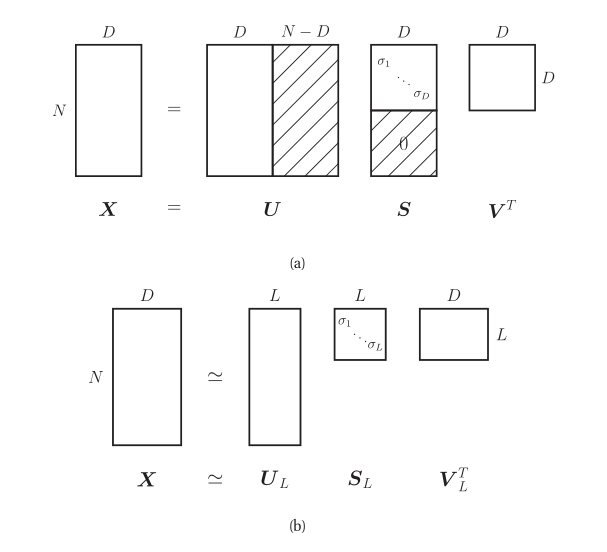
\includegraphics[width=0.7\linewidth]{fig/figure8}
	\caption*{图12.8:(a)非平方矩阵的奇异值分解$\X=\U\S\V^T$。$\S$的阴影部分和所有非对角项均为零。$\U$和$\S$中的阴影条目不在经济型版本中计算,因为它们不需要。(b) 秩L的截断奇异值分解近似。 }
\end{figure}

由于特征向量不受矩阵线性缩放的影响,我们可以看到$\S$的右奇异向量等于经验协方差$\textstyle\boldsymbol{\hat{\sum}}$的特征向量。此外,$\textstyle\boldsymbol{\hat{\sum}}$的特征值是平方奇异值的比例形式。这意味着我们只需要几行代码就可以执行PCA(参见pcaPmtk)。

然而,PCA和SVD之间的联系更深入。根据等式12.46,我们可以表示秩r矩阵,如下所示:
\begin{equation}
	\X=\sigma_1\left(\begin{array}{cccc}
	\mid  \\
	\u_1 \\
	\mid  
	\end{array} \right)(-\ \v_1^T\ -)+\dots
+\sigma_r\left(\begin{array}{cccc}
	\mid  \\
	\u_r \\
	\mid  
	\end{array} \right)(-\ \v_r^T\ -)\tag{12.54}
\end{equation}

如果奇异值如图12.10所示快速消失,我们可以生成矩阵的秩L近似值,如下所示: 

\begin{equation}
	\X\approx\U_{:,1:L}\ \S_{1:L,1:L}\ \V_{:,1:L}^T\tag{12.55}
\end{equation}

这称为\textbf{截断奇异值分解}(见图12.8(b))。使用秩L近似表示$N\times D$矩阵所需的参数总数为:
\begin{equation}
	NL+LD+L=L(N+D+1)\tag{12.56}
\end{equation}

\begin{figure}[h]
	\centering
	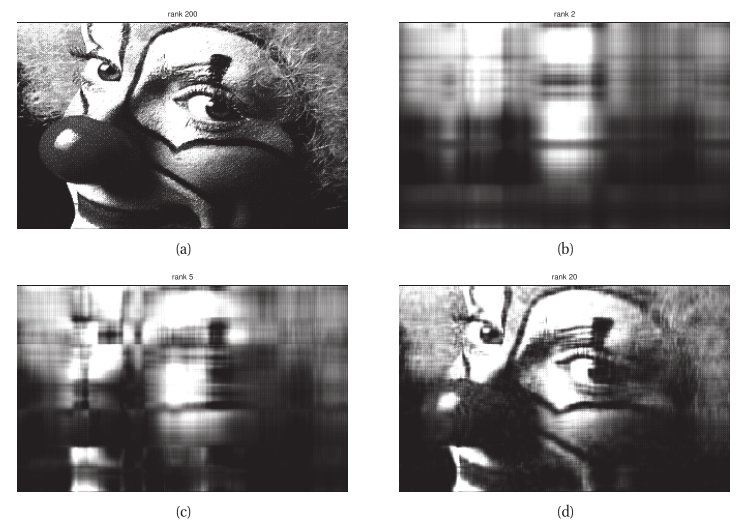
\includegraphics[width=0.7\linewidth]{fig/figure9}
	\caption*{图12.9: 图像的低秩近似。左上角:原始图像的大小为$200\times 320$,秩为200。后续图像的秩为2、5和20。由svdImageDemo生成的图。 }
\end{figure}

\begin{figure}[h]
	\centering
	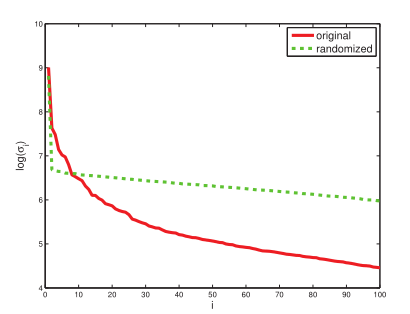
\includegraphics[width=0.7\linewidth]{fig/figure10}
	\caption*{图12.10: 粗略的图像的前50个对数奇异值(红色实线)和通过随机洗牌像素获得的数据矩阵(绿色虚线)。由svdImageDemo生成的图。  }
\end{figure}

例如,考虑图12.9(左上)中的$200\times 320$像素图像。这里面有64000个数字。我们看到秩近似20,只有$(200+320+1)20=10420$个数字是一个非常好的近似。


可以证明,该近似中的误差由以下公式得出:
\begin{equation}
	\parallel\X-\X_L\parallel_F\ \approx\ \sigma_{L+1}\tag{12.57}
\end{equation}

此外,可以证明奇异值分解为矩阵提供了最佳秩L近似(在最小化上述Frobenius范数的意义上最佳)。

让我们将其连接回PCA。设$\X=\U\S\V^T$是$\X$的截断奇异值分解。我们知道$\hat{\W}=\V$,并且$\hat{\Z}=\X\hat{\W}$,即:
\begin{equation}
	\hat{\Z}=\U\S\V^T\V=\U\S\tag{12.58}
\end{equation}

此外,最优重构由$\hat{\X}=\Z\hat{\W}^T$,我们得到:
 
\begin{equation}
	\hat{\X}=\U\S\V^T\tag{12.59}
\end{equation}

这与截断奇异值分解近似完全相同!这是另一个例子,说明PCA是数据的最佳低秩近似。

\clearpage
\subsubsection{概率主成分分析}

我们现在准备再次观测PPCA。可以显示以下显著结果。

\begin{mythm}\label{thm:light}
	((Tipping和Bishop,1999年))。考虑一个因子分析模型,其中$\boldsymbol{\varPsi}=\sigma^2\I$,$\W$是正交的。观察到的数据对数似然由以下公式得出: 
	
	
	\begin{equation}
	\log \ p(\X|\W,\sigma^2)\ \ =\ \ -\frac{N}{2}ln|\C|-\frac{1}{2}\sum_{i=1}^{N}\x_i^T\C^{-1}\x_i=-\frac{N}{2}ln|\C|+tr(\C^{-1}\textstyle\hat{\sum})\tag{12.60}
	\end{equation}
\end{mythm}

其中$\C=\W\W^T+\sigma^2\I$和$\S=\frac{1}{N}\sum\nolimits_{i=1}^N\x_i\x_i^T=(1/N)\X^T\X$。(为了符号简单起见,我们假设数据居中。)对数似然的最大值由下式得出:

\begin{equation}
	\hat{\W}=\V (\boldsymbol{\varLambda}-\sigma^2\I)^{\frac{1}{2}}\R\tag{12.61}
\end{equation}

其中$\R$是任意$L\times L$正交矩阵,$\V$是$D\times L$矩阵,其列是$\S$的前L个特征向量,$\varLambda$是特征值的对应对角矩阵。在不损失一般性的情况下,我们可以设置$\R=\I$。此外,噪声方差的最大似然估计由下式得出:

\begin{equation}
	\hat{\sigma}^2=\dfrac{1}{D-L}\sum_{j=L+1}^{D}\lambda_j\tag{12.62}
\end{equation}
这是与被抛弃的维度相关的平均方差。

因此,作为$\sigma^2\rightarrow0$,与经典的PCA相同。$\hat{\Z}$呢?很容易看出,潜在因素的后验值由以下公式得出:
\begin{align}
	p(\z_i|\x_i,\boldsymbol{\hat{\theta}})\ \ &=\ \ \mathcal{N}(\z_i|\hat{\F}^{-1}\hat{\W}^T\x_i,\sigma^2\hat{\F}^{-1})\tag{12.63}\\
	\hat{\F}\ \ &\triangleq\ \ \hat{\W}^T\hat{\W}+\hat{\sigma}^2\I\tag{12.64}
\end{align}

(不要将$\F=\W^T\W+\sigma^2\I$与$\C=\W\W^T+\sigma^2\I$混淆。)因此,作为$\sigma^2\rightarrow0$,我们找到$\hat{\W\rightarrow\V}$、$\hat{\F}\rightarrow\I$和$\hat{\z_i}\rightarrow\V^T\x_i$。因此,后验平均值是通过将数据正交投影到$\V$的列空间来获得的,与经典PCA中一样。

然而,请注意,如果$\sigma^2>$,则后验平均值不是正交投影,因为它向前验平均值收缩了一些,如图12.5(b)所示。这听起来像是一个不受欢迎的特性,但这意味着重建将更接近整体数据平均值,$\hat{\boldsymbol{\mu}}= \bar{\x}$。 

\subsubsection{PCA的EM算法}

虽然拟合主成分分析模型的通常方法使用特征向量方法或奇异值分解,但我们也可以使用EM,这将证明具有一些优势,我们将在下面讨论。主成分分析的EM依赖于主成分分析的概率公式。然而,该算法继续在零噪声限制下工作,$\sigma^2=0$,如(Roweis 1997)所示。 

设$\tbZ$是一个$L\times N$矩阵,沿其列存储后验均值(低维表示)。类似地,将原始数据沿其列存储。根据等式12.63,当$\sigma^2=0$时,我们有: 

\begin{equation}
	\tbZ=(\W^T\W)^{-1}\W^T\tbX\tag{12.65}
\end{equation}

这构成了E步骤。请注意,这只是数据的正交投影。

根据等式12.23,第M步长由下式得出:
\begin{equation}
	\hat{\W}\ \ =\ \ \left[\sum_{i}\x_i\mathbb{E}[\z_i]^T\right]\left[\sum_{i}\mathbb{E}[\z_i]\mathbb{E}[\z_i]^T\right]^{-1}\tag{12.66}
\end{equation}

在这里,我们利用了当$\sigma^2=0$时$\textstyle\boldsymbol{\sum}=cov[\z_i|\x_i,\theta]=0\I$的事实。值得将此表达式与多输出线性回归的最大似然估计进行比较(方程7.89),其形式为$\W\ =\ (\sum\nolimits_{i}\y_i\x_i^T)(\sum\nolimits_{i}\x_i\x_i^T)^{-1}$.因此,我们看到M步类似于线性回归,其中我们用潜在变量的预期值替换观察到的输入。 

总之,以下是整个算法:

\begin{itemize}
\item \textbf{第E步 $\tbZ=(\W^T\W)^{-1}\W^T\tbX$}
\item \textbf{第M步 $\W=\tbX\tbZ^T(\tbZ\tbZ^T)^{-1}$}
\end{itemize}

(Tipping和Bishop 1999)表明,EM算法的唯一稳定不动点是全局最优解。也就是说,EM算法收敛到一个解,其中$\W$跨越与第一个L特征向量定义的线性子空间相同的线性子空间。然而,如果我们希望$\W$是正交的,并且以特征值的降序包含特征向量,我们必须正交化得到的矩阵(这可以非常便宜地完成)。或者,我们可以修改EM以直接给出主基(Ahn和Oh 2003)。

该算法在$D=2$和$L=1$的情况下具有简单的物理类比(Roweis 1997)。考虑$\mathbb{R}^2$中由弹簧连接到刚性杆的一些点,其方向由向量$\w$定义。$z_i$是第i个弹簧连接到杆的位置。在E步骤中,我们固定杆,让附着点四处滑动,以最小化弹簧能量(与残差平方和成比例)。在M步骤中,我们固定附着点,让杆旋转,以最小化弹簧能量。请参见图12.11得到解释。 

\begin{figure}[h]
	\centering
	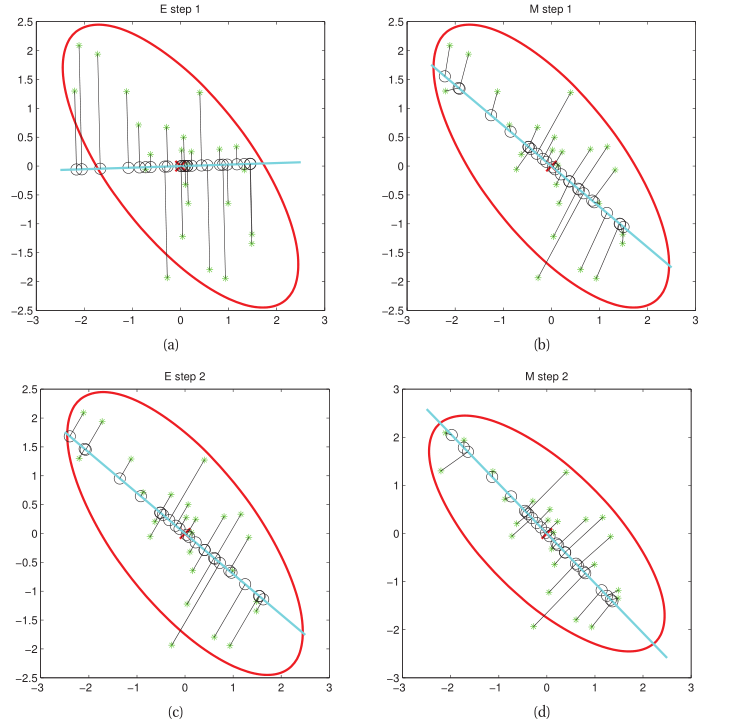
\includegraphics[width=0.7\linewidth]{fig/figure11}
	\caption*{图12.11: $D=2$和$L=1$时PCA的EM图示。绿星是原始数据点,黑圈是其重建。权重向量w由蓝线表示。(a) 我们从w的随机初始猜测开始。E步由正交投影表示。(b) 我们在M步骤中更新杆w,保持杆上的投影(黑色圆圈)固定。(c) 另一个E步骤。黑色圆圈可以沿杆“滑动”,但杆保持固定。(d) 另一个M步骤。基于(Bishop 2006b)的图12.12。pcaEmStepByStep生成的图。 }
\end{figure}

除了这种令人愉快的直观解释外,主成分分析的EM与特征向量方法相比具有以下优势: 
\begin{itemize}
\item  EM可以更快。特别是,假设$N,D \gg L$,EM的主要成本是E步骤中的投影操作,因此总时间为$O(TLND)$,其中T是迭代次数。(Roweis 1997)实验表明,无论N或D如何,迭代次数通常非常小(平均值为3.6)。(这一结果取决于经验协方差矩阵的特征值之比。)这比直接特征向量方法所需的$O(min(ND^2,DN^2))$时间快得多,尽管更复杂的特征向量方法,如Lanczos算法,其运行时间与EM相当。
\item EM可以以在线方式实现,也就是说,我们可以在数据流入时更新我们对$\W$的估计数据流。 
\item EM可以以简单的方式处理缺失数据(见第12.1.6节)。 
\item EM可以扩展到处理PPCA/FA模型的混合物。 
\item EM可以修改为变分EM或变分贝叶斯EM,以适应更复杂的模型。 
\end{itemize}

\begin{figure}[h]
	\centering
	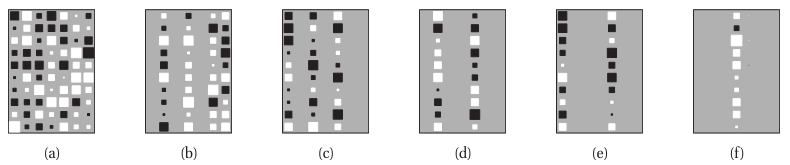
\includegraphics[width=0.7\linewidth]{fig/figure12}
	\caption*{图12.12: 使用VBEM估计混合因子分析仪中有效维数的图示。已通过ARD机制将空白列强制为0。数据来自6个内部维数为7、4、3、2、2、1的聚类,该方法已成功估计。资料来源:图4.4(Beal 2003)。经马特·比尔许可使用。 }
\end{figure}

\subsection{选择潜在维度的数量 }

在第11.5节中,我们讨论了如何在混合模型中选择组分K的数量。在本节中,我们讨论了如何在FA/PCA模型中选择潜在维数L的数量。
\subsubsection{FA/PPCA的模型选择 }

如果我们使用概率模型,原则上我们可以计算$L^*=argmax_Lp(L|D)$。然而,这有两个问题。首先,评估LVMs的边际可能性相当困难。在实践中,可以使用简单近似,例如BIC或变分下限(见第21.5节)(另请参见(Minka 2000a))。或者,我们可以使用交叉验证的可能性作为性能度量,尽管这可能很慢,因为它需要拟合每个模型F次,其中F是CV折叠的数量。

第二个问题是需要搜索潜在的大量模型。通常的方法是对L的所有候选值进行穷举搜索。然而,有时我们可以将模型设置为其最大大小,然后使用称为自动相关性确定(第13.7节)的技术,结合EM,自动删除不相关的权重。该技术将在第13章的监督上下文中描述,但可以适用于(M)FA上下文,如(Bishop 1999;Ghahramani和Beal 2000)所示。

\begin{figure}[h]
	\centering
	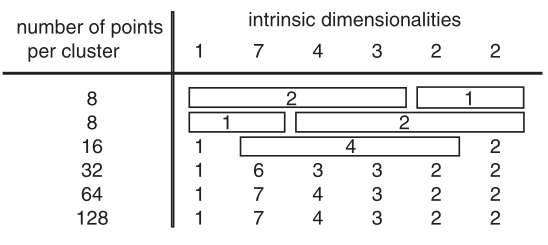
\includegraphics[width=0.7\linewidth]{fig/figure13}
	\caption*{图12.13: 显示了作为样本量函数的聚类估计数及其估计维数。当$N=8$时,VBEM算法找到了两个不同的解。注意,随着样本量的增加,发现了更多具有更大有效维数的簇。资料来源:表4.1(Beal 2003)。经马特·比尔善意许可使用。}
\end{figure}

图12.12说明了这种方法适用于适合小型合成数据集的混合FA。这些图使用\textbf{Hinton图}可视化了每个簇的权重矩阵,其中平方的大小与矩阵\footnote{杰夫·辛顿是托伦托大学计算机科学的英语教授。}中条目的值成比例。我们看到其中许多是稀疏的。图12.13显示稀疏度取决于训练数据量,符合贝叶斯Occam剃刀。特别是,当样本量较小时,该方法自动倾向于使用更简单的模型,但当样本量足够大时,该方法收敛于“正确”解,即具有维度1、2、2、3、4和7的6个子空间的解。

虽然ARD/EM方法很优雅,但它仍然需要在K上执行搜索。这是使用“出生”和“死亡”移动完成的(Ghahramani和Beal 2000)。另一种方法是在模型空间中进行随机抽样。传统方法,例如(Lopes和West 2004),基于可逆跳跃MCMC,也使用出生和死亡移动。然而,这可能很慢,很难实现。最近的方法使用非参数先验,结合吉布斯采样,例如(Paisley和Carin,2009)。

\subsubsection{主成分分析的模型选择}

由于主成分分析不是概率模型,我们不能使用上述任何方法。可能性的一个明显代表是重建误差:
\begin{equation}
	E(\mathcal{D},L)=\frac{1}{|\mathcal{D}|}\sum_{i\in \mathcal{D}}\parallel\x_i-\hat{\x}_i\parallel^2\tag{12.67}
\end{equation}
在主成分分析的情况下,重构由$\hat{\x}_i=\W\z_i+\boldsymbol{\mu}$,其中,$\z_i=\W^T(\x_i-\boldsymbol{\mu})$,$\W$和$\boldsymbol{\mu}$由$\mathcal{D}_{train}$估算。

\begin{figure}[h]
	\centering
	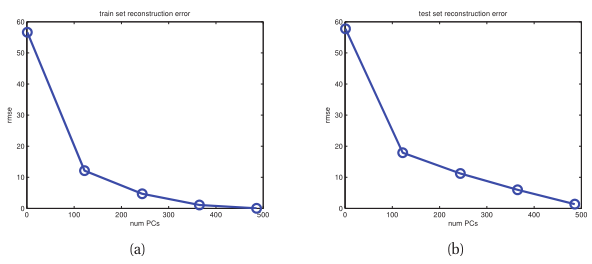
\includegraphics[width=0.7\linewidth]{fig/figure14}
	\caption*{图12.14:  MNIST的重建误差与主成分分析使用的潜在维数的数量。(a)训练集。(b)测试集。图由pcaOverfitDemo生成。}
\end{figure}

图12.14(a)绘制了图12.6中MNIST训练数据的$E(\mathcal{D}_{train},L)$与L。我们看到它下降得很快,这表明我们可以用少量因子捕捉像素的大部分经验相关性,如图12.6定性所示。

练习12.5要求您证明仅使用L项的残余误差由丢弃的特征值之和得出: 

\begin{equation}
	E(\mathcal{D}_{train},L)\ \ =\ \ \sum_{j=L+1}^{D}\lambda_j\tag{12.68}
\end{equation}
因此,替代绘制误差的方法是绘制保留的特征值,以递减的方式顺序。这被称为\textbf{scree图},因为 "该图看起来像一座山的侧面,而'scree'是指从山上掉下来的、躺在山脚下的碎石。指的是从山上掉下来的、躺在山脚下的碎片"。\footnote{来自:http://janda.org/workshop/factoranalysis/SPSSrun/SPSS08.htm.}形状与残余误差图相同。

相关量是解释的\textbf{方差分数},定义为:
\begin{equation}
	F(\mathcal{D}_{train},L)=\dfrac{\sum\nolimits_{j=1}^L\lambda_j}{\sum\nolimits_{j'=1}^{L_{max}}\lambda_{j'}}\tag{12.69}
\end{equation}
这与scree绘图捕获的信息相同。

当然,如果我们使用L=秩($\X$),我们在训练集上得到零重建误差。为了避免过度拟合,在测试集上绘制重建误差是很自然的。如图12.14(b)所示。在这里,我们看到,即使模型变得更复杂,误差仍在继续下降!因此,我们没有得到通常我们期望看到的U形曲线。

怎么回事?问题是主成分分析不是一个合适的数据生成模型。这只是一种压缩技术。如果你给它更多的潜在维度,它将能够更准确地近似测试数据。相比之下,概率模型具有贝叶斯-奥卡姆剃刀效应(第5.3.1节),即如果在数据较少的空间部分浪费概率质量,则会受到“惩罚”。这如图12.15所示,图中绘制了使用PPCA计算的负对数似然与L。在这里,在测试集上,我们看到了常见的U形曲线。 

\begin{figure}[h]
	\centering
	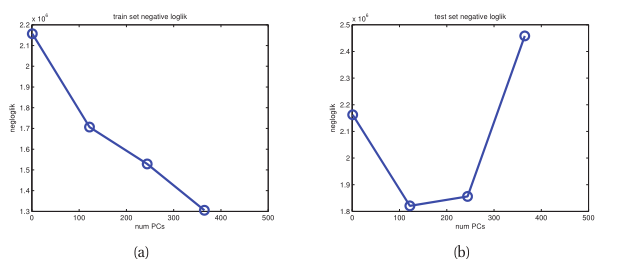
\includegraphics[width=0.7\linewidth]{fig/figure15}
	\caption*{图12.15:MNIST的负对数似然与PPCA使用的潜在维度数。(a)训练集。(b)测试集。图由pcaOverfitDemo生成。}
\end{figure}

这些结果与第11.5.2节中的结果类似,在第11.5.2节中,我们讨论了在K-means算法中选择K与使用GMM的问题。

\subsubsection*{12.3.2.1  \ Profile likelihood-轮廓可能性}
虽然没有U型曲线,但图中有时会出现“制度更迭”,从相对较大的误差到相对较小的误差。一种自动检测这种情况的方法在(zhu和Ghodsi 2006)中描述。想法是这样的。设$\lambda_k$是大小为k的模型产生的误差的某种度量,使得$\lambda_1\ge \lambda_2\ge ...\ge \lambda_{L_{max}}$。在主成分分析中,这些是特征值,但该方法也可以应用于K均值。现在考虑将这些值分为两组,这取决于$k<L$还是$k>L$,我们将确定一个阈值。为了测量L的质量,我们将使用一个简单的变点模型,其中如果$k\le L$,$\lambda_k\sim \mathcal{N}(\mu_2,\sigma^2)$如果$k>L$。(重要的是$\sigma^2$在两个模型中相同,以防止在一个区域的数据少于另一个区域的情况下过度拟合。)在这两个区域中,我们假设$\lambda_k$是iid,这显然是不正确的,但足以满足我们目前的目的。我们可以通过对数据进行分区并计算最大似然估计(MLE),使用方差的汇总估计,为每个$L=1:L_{max}$拟合该模型:

\begin{align}
	\mu_1(L)\ \ &=\ \ \dfrac{\sum\nolimits_{k\le L}\lambda_{k}}{L},\mu_2(L)\ \ =\ \ \dfrac{\sum\nolimits_{k> L}\lambda_{k}}{N-L}\tag{12.70}\\
	\sigma^2(L)\ \ &=\ \ \dfrac{\sum\nolimits_{k\le L}(\lambda_{k}-\mu_1(L))^2+\sum\nolimits_{k> L}(\lambda_{k}-\mu_2(L))^2}{N}\tag{12.71}
\end{align}
然后,我们可以评估\textbf{剖面对数的可能性}.
\begin{equation}
	\ell(L)\ \ =\ \ \sum_{k=1}^{L}\log \mathcal{N}(\lambda_k|\mu_1(L),\sigma^2(L))+\sum_{k=L+1}^{K}\log \mathcal{N}(\lambda_k|\mu_2(L),\sigma^2(L))\tag{12.72}
\end{equation}
最后,我们选择$L^*=arg\ max\ \ell(L)$。如图12.16所示。在左边,我们绘制了树状图,其形状与图12.14(a)中的形状相同。在右边,我们绘制了剖面图。


\begin{figure}[h]
	\centering
	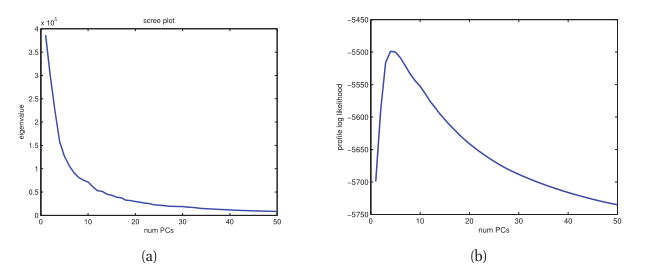
\includegraphics[width=0.7\linewidth]{fig/figure16}
	\caption*{图12.16: (a)对应于图12.14(a)的训练集的屏幕图。(b)轮廓可能性。图由pcaOverfitDemo生成。}
\end{figure}

\subsection{分类数据的PCA }
在本节中,我们考虑将因子分析模型扩展到观察数据为分类数据而非实值数据的情况。也就是说,数据的形式为$y_{ij}\in \{1,...,C\}$,其中$j=1:R$是观察到的响应变量的数量。我们假设每个$y_{ij}$由一个潜在变量$\z_i\in \mathbb{R}^L$生成,具有高斯先验,其通过softmax函数如下:
\begin{align}
	p(\z_i)\ \ &=\ \ \mathcal{N}(0,\I)\tag{12.73}\\
	p(\y_i|\z_i,\boldsymbol{\theta})\ \ &=\ \ \prod_{r=1}^{R}Cat(y_{ir}|S(\W_r^T\z_i+\w_{0r}))\tag{12.74}
\end{align}
其中$\W_r\in \mathbb{R}^{L\times M}$是响应$j$的因子载荷矩阵,$\w_{0r}\in \mathbb{R}^R$是响应r的偏移项和$\boldsymbol{\theta}=(\W_r,\w_{0r})_{r=1}^R$。(我们需要一个明确的偏移项,因为将$\z_i$的一个元素设置为1可能会在计算后验协方差时引起问题。)与因子分析一样,我们将先验均值定义为$\m_{\0}$,先验协方差$\V_0=\I$,因为我们可以通过改变$w_{0j}$来捕捉非零均值,通过改变$\W_r$来捕捉非同一协方差。我们将其称为\textbf{分类主成分分析}。有关相关模型的讨论,请参阅第27章。

有趣的是,研究通过改变参数,我们可以在观察变量上归纳出什么样的分布。为简单起见,我们假设存在单个三元响应变量,因此$y_i$存在在三维概率单纯形中。图12.17显示了当我们改变先验参数$\m_{0}$和$\V_0$时会发生什么,这相当于改变似然参数$\W_1$和$\w_{01}$。我们看到,这可以定义单纯形上相当复杂的分布。这种诱导分布称为\textbf{逻辑正态分布}(Aitchison 1982)。

我们可以使用EM的改进版本将该模型拟合到数据中。基本思想是在E步中推断后验$p(\z_i|\y_i,\boldsymbol{\theta})$的高斯近似,然后在M步中最大化$\boldsymbol{\theta}$。多类案例的详细信息见(Khan等人,2010)(另见第21.8.1.1节)。sigmoid链路的二进制情况的详细信息可以在练习21.9中找到,probit链路的详细信息可以在练习21.10中找到。

\begin{figure}[h]
	\centering
	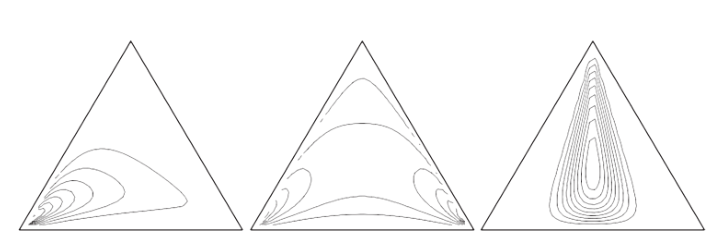
\includegraphics[width=0.7\linewidth]{fig/figure17}
	\caption*{图12.17: 在三维单线上定义的逻辑正态分布的一些示例。(a)对角协方差和非零均值。(b)状态1和2之间的负相关性。(c)状态1和2之间正相关。资料来源:图1(Blei和Lafferty 2007)。经David Blei善意许可使用。}
\end{figure}

\begin{figure}[h]
	\centering
	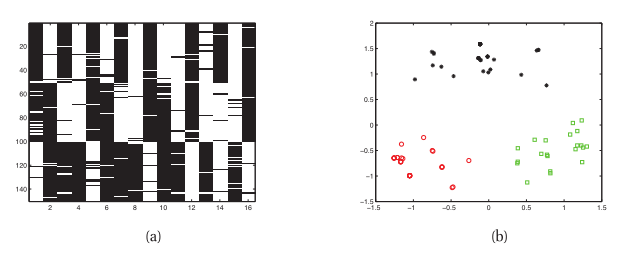
\includegraphics[width=0.7\linewidth]{fig/figure18}
	\caption*{图12.18: 左:150个合成16维位向量。右图:通过二进制PCA学习的2d嵌入,使用变分EM。我们根据生成它们的真实“原型”的身份获得颜色编码点。由binaryFaDemoTipping生成的图。}
\end{figure}

这种模型的一个应用是可视化高维分类数据。图12.18(a)显示了一个简单的示例,其中我们有150个6维位向量。很明显,每个样本只是三个二进制原型之一的嘈杂副本。我们将2d catFA拟合到该模型,得到近似的MLEs$\hat{\boldsymbol{\theta}}$。在图12.18(b)中,我们绘制了$\mathbb{E}{\LARGE [\z_i|\x_i,\hat{\boldsymbol{\theta}}]}$。正如预期的那样,我们看到有三个不同的集群。 

在(Khan等人,2010年)中,我们表明,该模型在填充由真实数据和分类数据组成的设计矩阵中的缺失项方面优于有限混合模型。这有助于分析社会科学调查数据,因为这些数据往往缺少数据和混合类型的变量。 

\begin{figure}[h]
	\centering
	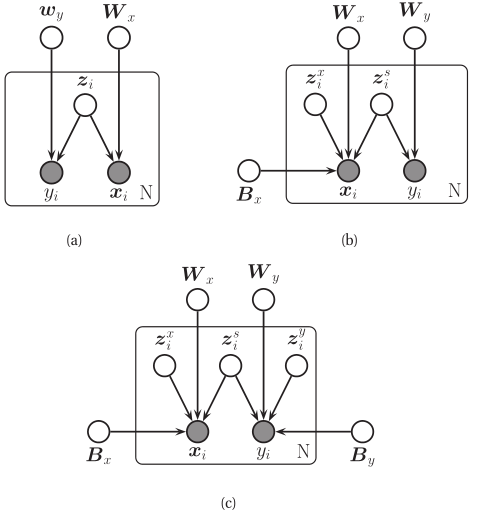
\includegraphics[width=0.5\linewidth]{fig/figure19}
	\caption*{图12.19: 成对数据的高斯潜在因子模型。(a) 有监督的PCA。(b) 偏最小二乘法。(c) 典范相关分析。}
\end{figure}

\subsection{成对和多视图数据的PCA}
通常会有一对相关数据集,例如基因表达和基因拷贝数,或用户的电影分级和电影评论。很自然地,我们希望将这些结合在一起,形成一个低维嵌入。这是数据融合的一个例子。在某些情况下,我们可能希望通过低维“瓶颈”从另一个元素$\x_{i2}$预测配对中的一个元素,例如$\x_{i1}$。 

下面,我们将在(Virtanen 2010)的介绍之后讨论这些任务的各种潜在高斯模型。对于$m=1:M$,模型很容易从成对推广到数据集$\x_{im}$,。我们重点讨论了$\x_{im}\in \mathbb{R}^{D_m}$的情况。在这种情况下,联合分布是多元高斯分布,因此我们可以使用EM或Gibbs采样拟合模型。 

正如我们在第27.2.2节中所解释的那样,我们可以通过使用指数族作为响应分布而不是高斯分布来概括模型,以处理离散和计数数据。然而,这将需要在E步骤中使用近似推理(或对MCMC的类似修改)。 

\subsubsection{监督PCA(潜在因子回归)}
考虑以下模型,如图12.19(a)所示:
\begin{align}
	p(\z_i)\ \ &=\ \ \mathcal{N}(\0,\I_L)\tag{12.75}\\
	p(y_i|\z_i)\ \ &=\ \ \mathcal{N}(\w_y^T\z_i+\mu_y,\sigma_y^2)\tag{12.76}\\
	p(\x_i|\z_i)\ \ &=\ \ \mathcal{N}(\W_x\z_i+\boldsymbol{\mu}_x,\sigma_x^2\I_D)\tag{12.77}
\end{align}
在(Yu等人,2006年)中,这被称为\textbf{监督PCA}。在(West 2003)中,这被称为\textbf{贝叶斯因子回归}。该模型类似于主成分分析,只是在学习低维嵌入时考虑了目标变量$y_i$。由于该模型是联合高斯模型,我们有:
\begin{equation}
	y_i|\x_i\ \ \sim\ \ \mathcal{N}(\x_i^T\w,\sigma_y^2+\w_y^T\C\w_y)\tag{12.78}
\end{equation}
其中$\w=\boldsymbol{\varPsi}^{-1}\W_x\C\w_y,\boldsymbol{\varPsi}=\sigma_x^2\I_D$,和$\C^{-1}=\I+\W_x^T\boldsymbol{\varPsi}^{-1}\W_x$。因此,虽然这是$(y_i,\x_i)$的联合密度模型,但我们可以推断出隐含的条件分布。

我们现在展示了一个与Zellner先验的有趣联系。假设$p(\w_y)=\mathcal{N}(\0,\frac{1}{g}\textstyle{\sum^2})$,并且假设$\X=\R\V^T$是$\X$的奇异值分解,其中$\V^T\V=\I$和$\R^T\R=\textstyle{\sum^2}=diag(\sigma_j^2)$包含平方奇异值。然后可以证明(West 2003)
\begin{equation}
	p(\w)=\mathcal{N}(\0,g\V^{-T}\boldsymbol{\textstyle{\sum^{-2}}}\V^{-1})=\mathcal{N}(\0,g(\X^T\X)^{-1})\tag{12.79}
\end{equation}
因此,$\w$对$\X$的先验依赖性来自于这样一个事实,即$\w$是通过$\X$和$\y$的联合模型间接推导出来的。 

上述讨论集中于回归。(Guo 2009)将CCA推广到指数族,如果$\x_i$和$y_i$是离散的,则更合适。虽然我们无法再以闭合形式计算条件$p(y_i|\x_i,\theta)$,但该模型具有与回归情况类似的解释,即我们通过潜在的“瓶颈”预测响应。 

压缩$\x_i$来预测$\y_i$的基本思想可以用信息论来表述。特别是,我们可能想找到一个编码分布$p(\z|\x)$,使我们最小化
\begin{equation}
	\mathbb{I}(\X;\Z)-\beta\mathbb{I}(\X;\Y)\tag{12.80}
\end{equation}
其中$\beta\ge0$是控制压缩和预测精度之间权衡的参数。这被称为\textbf{信息瓶颈}(Tishby等人,1999年)。通常Z被认为是离散的,如在聚类中。然而,在高斯情况下,IB与CCA密切相关(Chechik等人,2005年)。 

我们可以很容易地将CCA推广到$y_i$是要预测的反应的向量的情况,如在多标签分类中。(Ma等人,2008;Williamson和Ghahramani,2008)用这个模型来进行协作过滤,目标是预测$y_{ij}\in \{1,...,5\}$,即人的评分i对电影j的评价,其中的 "侧面信息 "$x_i$采取了i的朋友名单的形式。这种方法背后的直觉是这种方法背后的直觉是,了解你的朋友是谁,以及所有其他用户的评级以及所有其他用户的评分,应该有助于预测你会喜欢哪些电影。一般来说,任何任务相关的环境任务是相关的,都可以从CCA中受益。一旦我们采用了概率论的观点,各种扩展是直接的。例如,我们可以很容易地推广到半监督式的的情况下,我们不能对所有的i都观察到$\y_i$(Yu等人,2006)。

\subsubsection*{12.5.1.1  判别监督主成分分析 }
该模型的一个问题是,它在预测输入$\x_i$和输出$\y_i$上的权重相同。这可以通过使用以下形式的加权目标来部分缓解(Rish等人,2008年): 
\begin{equation}
	\ell (\boldsymbol{\theta})=\displaystyle{\prod_{i}}p(\y_i|\boldsymbol{\eta}_{iy})^{\alpha_y }p(\x_i|\boldsymbol{\eta}_{ix})^{\alpha_x}\tag{12.81}
\end{equation}
其中$\alpha_m$控制数据源的相对重要性,$\boldsymbol{\eta}_{im}=\W_m\z_i$。对于高斯数据,我们可以看到$\alpha_m$仅控制噪声方差: 
\begin{equation}
	\ell (\boldsymbol{\theta}) \propto \displaystyle{\prod_{i}} exp(-\frac{1}{2}\alpha_x||\x_i^T-\boldsymbol{\eta}_{ix}||^2)exp(-\frac{1}{2}\alpha_y||\y_i^T-\boldsymbol{\eta}_{iy}||^2)\tag{12.82}
\end{equation}
这种解释更普遍地适用于指数族。然而,请注意,很难估计$\alpha_m$参数,因为改变它们会改变似然的归一化常数。我们给出了一种替代方法,以在下面更重地加权$\y$。 
\subsubsection{偏最小二乘法}
\textbf{偏最小二乘法(PLS)(}Gustafsson 2001;Sun等人,2009)是监督主成分分析的一种不对称或更具“判别性”的形式。关键思想是允许输入特征中的一些(co)方差由其自身的子空间$\z_i^x$解释,并允许子空间$\z_i^s$的其余部分在输入和输出之间共享。模型具有以下形式:
\begin{align}
	p(\z_i)\ \ &=\ \ \mathcal{N}(\z_{i}^s|\0,\I_{L_s})\mathcal{N}(\z_i^x|\0,\I_{L_x})\tag{12.83}\\
	p(\y_i|\z_i)\ \ &=\ \ \mathcal{N}(\W_y\z_{i}^s+\boldsymbol{\mu}_y,\sigma^2\I_{D_y})\tag{12.84}\\
	p(\x_i|\z_i)\ \ &=\ \ \mathcal{N}(\W_x\z_{i}^s+\B_x\z_i^x+\boldsymbol{\mu}_x,\sigma^2\I_{D_x})\tag{12.85}
\end{align}
见图12.19(b)。可见变量上的相应诱导分布具有以下形式: 
\begin{equation}
	p(\v_i|\boldsymbol{\theta})=\int \mathcal{N}(\v_i|\W\z_i+\boldsymbol{\mu},\sigma^2\I)\mathcal{N}(\z_i|\0,\I)d\z_i=\mathcal{N}(\v_i|\boldsymbol{\mu},\W\W^T+\sigma^2\I)\tag{12.86}
\end{equation}
其中$\v_i=(\x_i;\y_i),\boldsymbol{\mu}=(\boldsymbol{\mu}_y;\boldsymbol{\mu}_x)$和
\begin{align}
	\mathbf{W} \ \ &=\ \  \left(
	\begin{array}{cccc}
	\W_y & 0  \\
	\W_x & \B_x \\
	\end{array} \right)\tag{12.87}\\
	\mathbf{W}\W^T \ \ &=\ \  \left(
	\begin{array}{cccc}
	\W_y\W_y^T & \W_x\W_x^T  \\
	\W_x\W_x^T & \W_x\W_x^T+\B_x\B_x^T \\
	\end{array} \right)\tag{12.88}
\end{align}
我们应该选择足够大的L,以使共享子空间不捕捉协变量特异性变化。 

使用指数族可以很容易地将该模型推广到离散数据(Virtanen 2010)。 
\subsubsection{典型相关分析}
\textbf{典型相关分析(CCA)}类似于PLS的对称无监督版本:它允许每个视图都有自己的“私有”子空间,但也有一个共享子空间。如果我们有两个观察变量,$\x_i$和$\y_i$,那么我们有三个潜在变量,$\z_i^s\in \mathbb{R}^{L_0}$是共享的,$\z_i^x\in \mathbb{R}^{L_x}$和$\z_i^y\in \mathbb{R}^{L_y}$这是私人的。我们可以将模型编写如下(Bach和Jordan 2005):
\begin{align}
	p(\z_i)\ \ &=\ \ \mathcal{N}(\z_{i}^s|\0,\I_{L_s})\mathcal{N}(\z_i^x|\0,\I_{L_x})\mathcal{N}(\z_i^y|\0,\I_{L_y})\tag{12.89}\\
	p(\x_i|\z_i)\ \ &=\ \ \mathcal{N}(\x_i|\B_x\z_i^x+\W_x\z_{i}^s+\boldsymbol{\mu}_x,\sigma^2\I_{D_x})\tag{12.90}\\
	p(\y_i|\z_i)\ \ &=\ \ \mathcal{N}(\y_i|\B_y\z_i^y+\W_y\z_{i}^s+\boldsymbol{\mu}_y,\sigma^2\I_{D_y})\tag{12.91}
\end{align}
见图12.19(c)。相应的观察到的联合分布具有以下形式 
\begin{equation}
p(\v_i|\boldsymbol{\theta})=\int \mathcal{N}(\v_i|\W\z_i+\boldsymbol{\mu},\sigma^2\I)\mathcal{N}(\z_i|\0,\I)d\z_i=\mathcal{N}(\v_i|\boldsymbol{\mu},\W\W^T+\sigma^2\I_D)\tag{12.92}
\end{equation}
其中:
\begin{align}
\mathbf{W} \ \ &=\ \  \left(
\begin{array}{cccc}
\W_x &\B_x &0  \\
\W_y &0 & \B_y \\
\end{array} \right)\tag{12.93}\\
\mathbf{W}\W^T \ \ &=\ \  \left(
\begin{array}{cccc}
\W_x\W_x^T+\B_x\B_x^T & \W_x\W_y^T \\
\W_y\W_y^T & \W_y\W_y^T+\B_y\B_y^T  \\
\end{array} \right)\tag{12.94}
\end{align}
可以使用EM计算该模型的最大似然估计。(Bach和Jordan 2005)表明,得到的最大似然估计等价于(旋转和缩放)经典的非概率视图。然而,概率观点的优点很多:我们可以简单地推广到$M>2$个观察变量;我们可以创建CCA的混合物(Viinikanoja等人,2010年);我们可以使用ARD创建CCA的稀疏版本(Archambeau和Bach 2008);我们可以推广到指数族(Klami等人,2010);我们可以对参数进行贝叶斯推断(WQang2007;Klami和Kaski 2008);我们可以处理$\W$和$\B$的非参数稀疏性提升先验(Rai和Daume 2009);等等。
\subsection{独立分量分析(ICA)}
考虑以下情况。你在一个拥挤的房间里,很多人在说话。我们的耳朵基本上就像两个麦克风,它们在听房间里不同语音信号的线性组合。我们的目标是将混合信号分解为其组成部分。这被称为\textbf{鸡尾酒会问题},是\textbf{盲信号分离(BSS)或盲源分离}的一个示例,其中“盲”表示我们对信号源“一无所知”。除了在声学信号处理中的明显应用外,在分析EEG和MEG信号、财务数据和任何其他潜在源或因素以线性方式混合在一起的数据集(不一定是暂时的)时,也会出现这个问题。 

我们可以将问题形式化如下。让$\x_t\in \mathbb{R}^D$是“时间”t时传感器上的观察信号,$\z_t\in \mathbb{R}^L$是源信号的矢量。我们假设 
\begin{equation}
	\x_t=\W\z_t+\epsilon_t\tag{12.95}
\end{equation}

\begin{figure}[h]
	\centering
	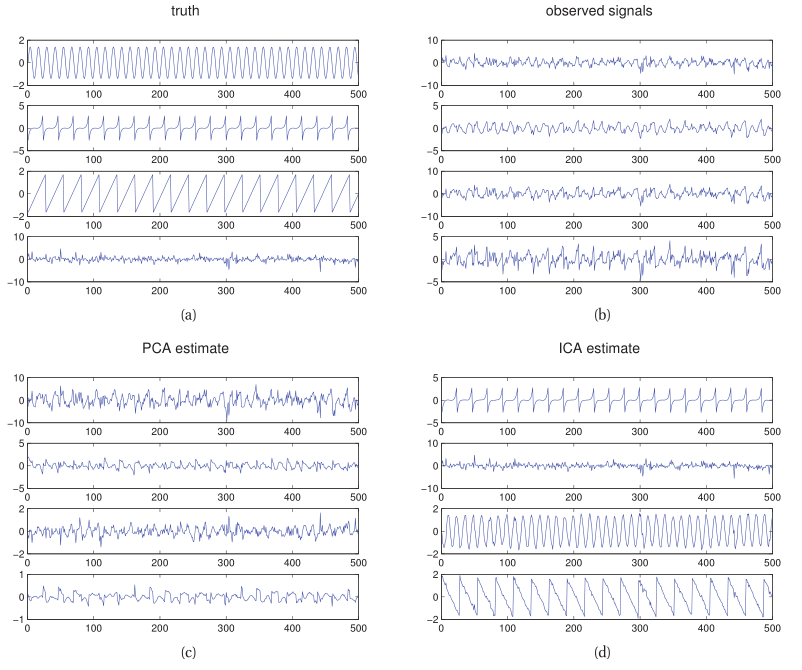
\includegraphics[width=0.7\linewidth]{fig/figure20}
	\caption*{图12.20: ICA应用于4d源信号的500个iid样本的图示。(a)潜在信号。(b)观察结果。(c)主成分分析估计。(d) ICA估计。图由icaDemo生成,由Aapo Hyvarinen编写。}
\end{figure}
其中$\W$是$D\times L$矩阵,并且$\epsilon_t\sim\mathcal{N}(\0,\boldsymbol{\varPsi})$。在本节中,我们将每个时间点视为一个独立的观察值,即我们不建模时间相关性(因此我们可以用i代替t指数,但我们坚持用t与许多独立分量分析文献一致)。目标是推断源信号$p(\z_t|\x_t,\boldsymbol{\theta})$,如图12.20所示。在这种情况下,$\W$被称为\textbf{混合矩阵}。如果$L=D$(信源数量=传感器数量),则它将是一个方阵。为了简单起见,我们通常假设噪声级$|\boldsymbol{\varPsi}|$为零。 

到目前为止,该模型与因子分析(如果没有噪声,则为PCA)相同,但我们通常不需要$\W$的正交性。然而,我们将对$p(\z_t)$使用不同的先验。在主成分分析中,我们假设每个信源是独立的,并且具有高斯分布 
\begin{equation}
	p(\z_t)=\prod_{j=1}^{L}\mathcal{N}(z_{tj}|0,,1)\tag{12.96}
\end{equation}

现在,我们将放松这个高斯假设,并让源分布为任何非高斯分布
\begin{equation}
	p(\z_t)=\prod_{j=1}^Lp_j(z_{tj})\tag{12.97}
\end{equation}
\begin{figure}[h]
	\centering
	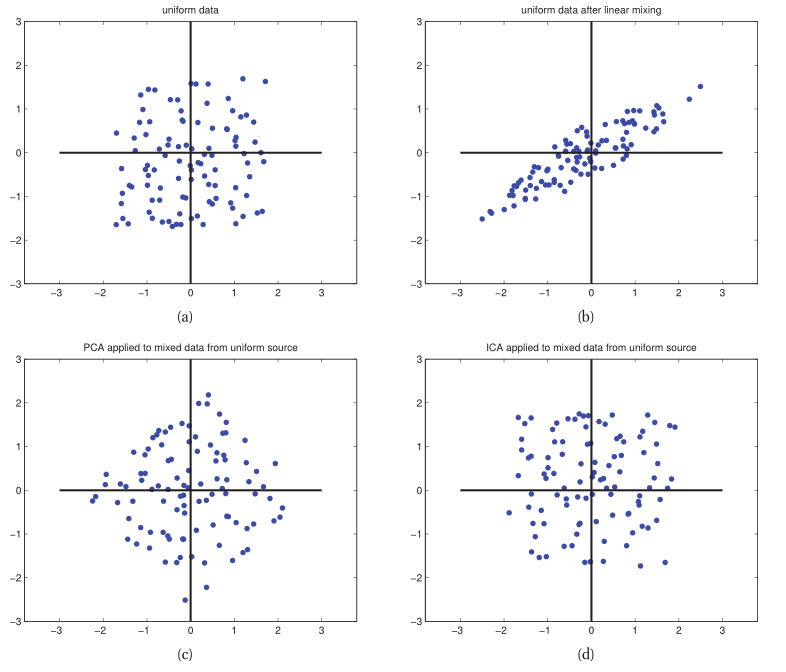
\includegraphics[width=0.7\linewidth]{fig/figure21}
	\caption*{图12.21: 对均匀分布的2d源信号的100个iid样本应用独立分量分析和主成分分析的图示。(a) 潜在信号。(b) 观察结果。(c) 主成分分析估计。(d) ICA估计。图由icaDemoUniform生成,由Aapo Hyvarinen编写。 }
\end{figure}

在不丧失一般性的情况下,我们可以将源分布的方差限制为1,因为任何其他方差都可以通过适当地缩放$\W$的来建模。由此产生的模型称为\textbf{独立分量分析(ICA)}。

高斯分布在独立分量分析中不允许作为信源先验的原因是,它不允许信源的唯一恢复,如图12.20(c)所示。这是因为PCA似然对源$\z_t$和混合矩阵$\W$的任何正交变换都是不变的。PCA可以恢复信号所在的最佳线性子空间,但不能唯一地恢复信号本身。 

为了说明这一点,假设我们有两个均匀分布的独立源,如图12.21(a)所示。现在假设我们有以下混合矩阵 
\begin{equation}
	\W=\left(
	\begin{array}{cccc}
	2 & 3\\
	2 & 1\\
	\end{array}\right)\tag{12.98}
\end{equation}
然后,我们观察图12.21(b)中所示的数据(假设没有噪声)。如果我们应用PCA,然后对其进行缩放,我们得到的结果如图12.21(c)所示。这对应于数据的白化。为了唯一地恢复信源,我们需要执行额外的旋转。问题是,对称高斯后验中没有信息告诉我们旋转的角度。在某种意义上,主成分分析解决了问题的“一半”,因为它识别了线性子空间;ICA所要做的就是识别适当的旋转。(因此,我们发现独立分量分析与varimax等方法没有太大不同,后者寻求潜在因子的良好旋转,以增强可解释性。) 

图12.21(d)表明,独立分量分析可以恢复信源,直至索引排列和可能的符号变化。独立分量分析要求$\W$是平方的,因此是可逆的。在非平方情况下(例如,我们的信源比传感器多),我们无法唯一地恢复真实信号,但我们可以计算后验$p(\z_t|\x_t,\hat{W})$,它表示我们对信源的信任。在这两种情况下,我们需要估计$\W$以及源分布$p_j$。我们在下面讨论如何做到这一点。 

\subsubsection{最大似然估计 }
在本节中,我们讨论了无噪声ICA模型的平方混合矩阵$\W$的估计方法。像往常一样,我们假设观察结果已经居中;因此,我们也可以假设$\z$是零均值。此外,我们假设观察值经过白化处理,这可以通过主成分分析完成。 

如果数据居中并白化处理,我们有$\mathbb{E}[\x\x^T]=\I$。但在无噪声的情况下,我们也有 
\begin{equation}
	cov[\x]=\mathbb{E}[\x\x^T]=\W\mathbb{E}[\z\z^T]\W^T=\W\W^T\tag{12.99}
\end{equation}
因此我们看到$\W$必须是正交的。这将我们必须估计的参数数量从$D^2$减少到$D(D-1)/2$. 它还将简化数学和算法。 

设$\V=\W^{-1}$,这些通常被称为\textbf{识别权重},而$\W$是\textbf{生成权重}\footnote{在文献中,通常用$\A$表示生成权重,用$\W$表示识别权重,但我们试图与本章前面使用的符号保持一致。 }。 

由于$\x=\W\z$,我们从等式2.89中得到:
\begin{equation}
	p_x(\W\z_t)=p_z(\z_t)|det(\W^{-1})|=p_z(\V\x_t)|det(\V)|\tag{12.100}
\end{equation}
因此,假设T iid样本,我们可以写出对数似然,如下所示: 
\begin{equation}
	\frac{1}{T}\log p(\mathcal{D}|\V)=\log |det(\V)|+\frac{1}{T}\sum_{j=1}^{L}\sum_{t=1}^{T}\log p_j(\v_j^T\x_t)\tag{12.101}
\end{equation}
其中,$\v_j$是$\V$的第j行。由于我们将$\V$约束为正交,第一项是常数,因此我们可以去掉它。我们还可以用期望值替换数据的平均值,以实现以下目标 
\begin{equation}
	NLL(\V)=\sum_{j=1}^{L}\mathbb{E}[\G_j(\z_j)]\tag{12.102}
\end{equation}
其中$z_j=\v_j^T\x$和$G_j(z)\triangleq
-\log p_j(z)$。我们希望最小化这个主题,使$\V$的行正交。我们还希望它们是单位范数,因为这确保了因子的方差是统一的(因为,对于白化数据,$\mathbb{E}[\v_j^T\x]=\parallel\v_j \parallel^2$,这是固定权重比例所必需的。换句话说,$\V$应该是正交矩阵。 

推导出适合该模型的梯度下降算法很简单;然而,这相当缓慢。我们还可以推导出一种遵循自然梯度的更快算法;详见(MacKay 2003,第34章)。一种流行的替代方法是使用近似牛顿法,我们在第12.6.2节中讨论了该方法。另一种方法是使用EM,我们将在第12.6.3节中讨论。 

\subsubsection{FastICA算法 }
现在,我们描述了基于(Hyvarinen和Oja 2000)的\textbf{快速ICA算法},我们将展示用于拟合ICA模型的近似牛顿法。 

为了简单起见,我们最初假设只有一个潜在因素。此外,我们最初假设所有信源分布都是已知的并且是相同的,因此我们可以只写$G(z)=-\log p(z)$。设$g(z)=\frac{d}{dz}G(z)$约束目标及其梯度和Hessian由下式给出: 
\begin{align}
	f(\v)\ \ &=\ \ \mathbb{E}[G(\v^T\x)]+\lambda(1-\v^T\v)\tag{12.103}\\
	\nabla f(\v)\ \ &=\ \ \mathbb{E}[\x g(\v^T\x)]-\beta\v\tag{12.104}\\
	\H(\v)\ \ &=\ \ \mathbb{E}[\x\x^Tg'(\v^T\x)]-\beta\I\tag{12.105}
\end{align}
其中$\beta =2\lambda$是拉格朗日乘子。让我们进行近似 
\begin{equation}
	\mathbb{E}[\x\x^Tg'(\v^T\x)]\approx \mathbb{E}[\x\x^T]\mathbb{E}[g'(\v^T\x)]=\mathbb{E}[g'(\v^T\x)]\tag{12.106}
\end{equation}
这使得Hessian函数非常容易反转,从而产生以下牛顿更新:
\begin{equation}
	\v^* \triangleq \v -\dfrac{\mathbb{E}[\x g(\v^T\x)]-\beta \v}{\mathbb{E}[g'(\v^T\x)]-\beta} \tag{12.107}
\end{equation}
可以用以下方式重写 
\begin{equation}
\v^* \triangleq \mathbb{E}[\x g(\v^T\x)] -\mathbb{E}[g'(\v^T\x)]\v \tag{12.108}
\end{equation}
(在实践中,可以用训练集的 Monte Carlo 估计值代替期望值,这提供了一种有效的在线学习算法。)执行此更新后,应使用 
\begin{equation}
	\v^{new}\triangleq \dfrac{\v^*}{||\v^*||}\tag{12.109}
\end{equation}
\begin{figure}[h]
	\centering
	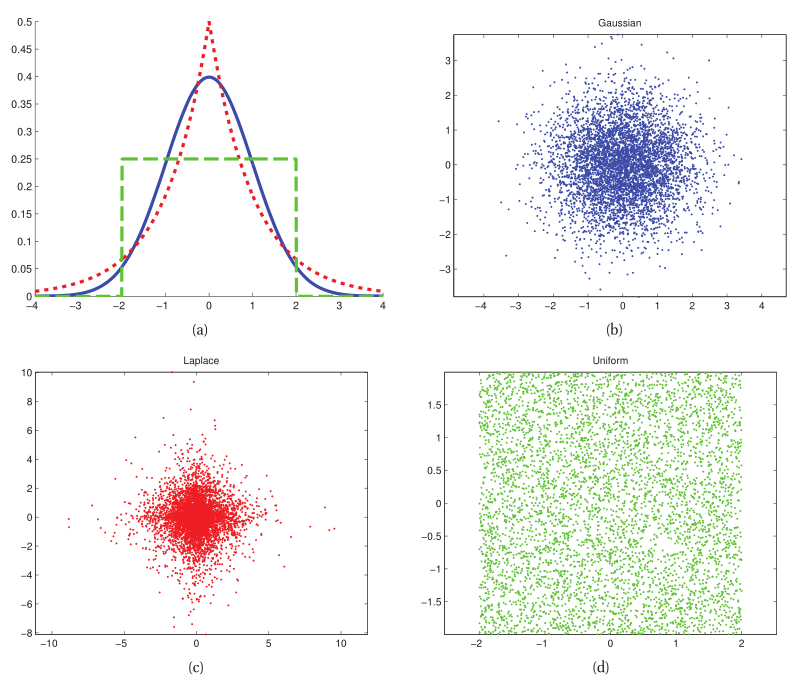
\includegraphics[width=0.7\linewidth]{fig/figure22}
	\caption*{图12.22: 1d和2d中高斯、亚高斯(均匀)和超高斯(拉普拉斯)分布的图示。图由凯文·斯沃斯基(KevinSwersky)编写的subSuperGaussPlot生成。 }
\end{figure}

迭代该算法直到收敛。(由于v的符号模糊性,$\v$的值可能不会收敛,但该向量定义的方向应收敛,因此可以通过监测$|\v^T\v^{new}|$来评估收敛性,该值应接近1。) 

由于目标不是凸的,因此存在多个局部最优解。我们可以利用这个结果来学习多个不同的权重向量或\textbf{特征}。我们可以依次学习特征,然后投影出位于由早期特征定义的子空间中的$\v_j$部分,或者我们可以并行学习它们,并行正交化$\V$。后一种方法通常是首选的,因为与PCA不同,特征不以任何方式排序。因此,第一个特征并不比第二个特征“更重要”,因此最好对称地处理它们。 

\subsubsection*{12.6.2.1 模拟源密度 }
到目前为止,我们假设$G(z)=-\log p(z)$是已知的。什么样的模型可能是合理的信号先验?我们知道使用高斯(对应于G的二次函数)是行不通的。所以我们需要某种非高斯分布。通常,有几种非高斯分布,例如: 
\begin{itemize}
	\item \textbf{超高斯分布} 这些分布在平均值处有一个大尖峰,因此(为了确保单位方差)有重尾。拉普拉斯分布是一个典型的例子。见图12.22。形式上,如果$kurt(z)>0$,我们称分布为\textbf{超高斯或leptokurtic}(“lepto”来自希腊语,表示“瘦”),其中kurt(z)是分布的\textbf{峰度},定义如下: 
	\begin{equation}
		kurt(z)\triangleq\frac{\mu_4}{\sigma^4}-3\tag{12.110}
	\end{equation}
	其中$\sigma$是标准差,$\mu_k$是第k个中心力矩,或关于平均值的力矩: 
	\begin{equation}
		\mu_k\triangleq\mathbb{E}[(\X-\mathbb{E}[\X])^k]\tag{12.111}
	\end{equation}
	(因此$\mu_1=\mu$是平均值,$\mu_2=\sigma^2$是方差。)通常在峰度定义中减去3,使高斯变量的峰度等于零。 
	\item \textbf{亚高斯分布亚高斯或平谷分布}(“平谷”来自希腊语,表示“宽”)具有负峰度。这些分布比高斯分布平坦得多。均匀分布是一个典型的例子。见图12.22。 
	\item \textbf{偏态分布}“非高斯”的另一种方式是不对称。其中一个度量是\textbf{偏度},由 
	\begin{equation}
		skew(z)\triangleq\frac{\mu_3}{\sigma^3}\tag{12.112}
	\end{equation}
\end{itemize}

(右)偏态分布的一个例子是伽马分布(见图2.9)。

当我们观察许多自然信号(如图像和语音)的经验分布时,当通过某些线性滤波器时,它们往往是超高斯的。这一结果既适用于在大脑某些部位发现的线性滤波器,如初级视觉皮层中发现的简单细胞,也适用于信号处理中使用的线性滤波器,如小波变换。因此,使用独立分量分析对自然信号建模的一个明显选择是拉普拉斯分布。对于均值零和方差1,其对数pdf由以下公式得出: 
\begin{equation}
	\log p(z)=-\sqrt{2}|z|-\log (\sqrt{2})\tag{12.113}
\end{equation}
由于拉普拉斯先验在原点不可微,因此更常见的是使用其他更平滑的超高斯分布。一个例子是逻辑分布。对应的对数pdf,对于平均值为零,方差为1的情况(因此$\mu=0,s=\frac{\sqrt{3}}{\pi}$),由以下公式得出: 
\begin{equation}
	\log p(z)=-2\log cosh(\frac{\pi}{2\sqrt{3}}z)-\log \frac{4\sqrt{3}}{\pi}\tag{12.114}
\end{equation}
\begin{figure}[h]
	\centering
	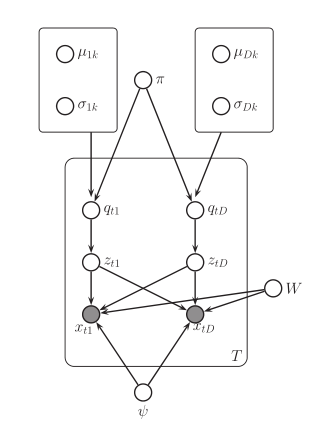
\includegraphics[width=0.4\linewidth]{fig/figure23}
	\caption*{图12.23: 使用单变量高斯混合建模源分布(的独立因子分析模型(Moulines等人,1997;Attias 1999))。 }
\end{figure}

估计$G(Z)=-\log p(z)$在开创性论文(Pham和Garrat 1997)中进行了讨论。然而,当通过最大似然法拟合独立分量分析时,知道信源分布的准确形状并不重要(尽管知道它是亚高斯分布还是超高斯分布很重要)。因此,通常只使用$G(z)=\sqrt{z}$或$G(z)=\log cosh(z)$,而不是上面更复杂的表达式。 
\subsubsection{使用EM }
假设$G(z)$的特定形式或$p(z)$的等效形式的替代方法是使用灵活的非参数密度估计器,例如(单变量)高斯的混合物: 
\begin{align}
	p(q_j=k)\ \ &=\ \ \pi_k\tag{12.115}\\
	p(z_j|q_j=k)\ \ &=\ \ \mathcal{N}(\mu_{j,k},\sigma_{j,k}^2)\tag{12.116}\\
	p(\x|\z)\ \ &=\ \ \mathcal{N}(\W\z,\boldsymbol{\varPsi})\tag{12.117}
\end{align}
这种方法是在(Moulines等人,1997年;Attias 1999年)中提出的,相应的图形模型如图12.23所示。 

对于这个模型,有可能推导出一个精确的EM算法。关键的观察是,可以通过对$\q_t$变量的所有$K^L$组合求和来精确计算$\mathbb{E}[\z_t|\x_t,\boldsymbol{\theta}]$,其中K是每个源的混合成分的数量。(如果这个方法太昂贵,可以使用变异平均场近似法(Attias 1999))。然后,我们可以通过对$\mathbb{E}[\z_t]$进行标准的GMM拟合来估计所有的源分布。当源的GMMs已知时,我们可以非常容易地计算边际$p_j(z_j)$,使用
\begin{equation}
	p_j(z_j)=\sum_{k=1}^{K}\pi_{j,k}\mathcal{N}(z_j|\mu_{j,k},\sigma_{j,k}^2)\tag{12.118}
\end{equation}
给定$p_j$,我们可以使用独立分量分析算法来估计$\W$。当然,这些步骤应该交错进行。详情见(Attias 1999)。 
\subsubsection{其他估算原则* }
使用与最大似然法不同的方法估计独立分量分析模型的参数是很常见的。我们将在下面回顾其中一些方法,因为它们为独立分量分析提供了更多的见解。然而,我们也将看到,这些方法实际上毕竟等价于最大似然法。我们的介绍基于(Hyvarinen和Oja 2000)。

\subsubsection*{12.6.4.1  最大限度地提高非高斯性 }
独立分量分析的早期方法是找到矩阵$\V$,使分布$\z=\V \x$尽可能远离高斯分布。(统计学中有一种相关方法称为投影寻踪。)非高斯性的一个度量是峰度,但这可能对异常值敏感。另一个度量是\textbf{负熵},定义为 
\begin{equation}
	negentropy(z) \triangleq \mathbb{H}(\mathcal{N}(\mu,\sigma^2))-\mathbb{H}(z)\tag{12.119}
\end{equation}
其中$\mu=\mathbb{E}[z]$和$\sigma^2=var[z]$。由于高斯分布是最大熵分布,因此该测度总是非负的,对于高度非高斯的分布,该测度会变大。 

我们可以将目标定义为最大化 
\begin{equation}
	J(\V)=\sum_{j}negentropy(z_j)=\sum_{j}\mathbb{H}(\mathcal{N}(\mu_j,\sigma_j^2))-\mathbb{H}(z_j)\tag{12.120}
\end{equation}
其中$\z=\V\x$。如果我们将$\V$固定为正交,并且如果我们将数据白化处理,$\z$的协方差将是独立于$\V$的$\I$,因此第一项是常数。因此 
\begin{equation}
	J(\V)=\sum_j-\mathbb{H}(z_j)+const=\sum_j\mathbb{E}[\log p(z_j)]+const\tag{12.121}
\end{equation}
我们看到它等于(符号变化和无关常数)等式12.102中的似然对数。

\subsubsection*{12.6.4.2  最大限度地减少相互信息}
一组随机变量的依赖性的一个衡量标准是\textbf{多信息的}。
\begin{equation}
	\I(\z)\triangleq\mathbb{K}\mathbb{L}\left(p(\z)||\prod_j p(z_j)\right)=\sum_j\mathbb{H}(z_j)-\mathbb{H}(\z)\tag{12.122}
\end{equation}
我们希望尽量减少这种情况,因为我们正在努力寻找独立的组件。换句话说,我们希望得到联合分布的最佳因子近似值。 

既然$\z=\V\x$,那么 
\begin{equation}
	\mathit{I}(\z)=\sum_j\mathbb{H}(z_j)-\mathbb{H}(\V\x)\tag{12.123}
\end{equation}

如果我们将$\V$约束为正交,我们可以去掉最后一项,因为$\mathbb{H}(\V\x)=\mathbb{H}(\x)$因为乘以$\V$不会改变分布的形状),而$\mathbb{H}(\x)$是一个常数,仅由经验分布决定。因此我们有$\mathit{I}(\z)=\sum_j\mathbb{H}(z_j)$。最小化这一点相当于最大化负熵,这相当于最大似然。 

\subsubsection*{12.6.4.3 最大化相互信息(infomax)}
与其试图最小化$\z$分量之间的互信息,不如想象一个神经网络,其中$\x$是输入,$y_i=\phi (\v_j^T)+\epsilon$是噪声输出,其中$\phi$是一些非线性标量函数,和$\epsilon\sim \mathcal{N}(0,1)$。试图最大化通过该系统的信息流似乎是合理的,这一原则被称为\textbf{infomax}。(Bell和Sejnowski 1995)。也就是说,我们希望最大化$\y$(内部神经表示)和$\x$(观察到的输入信号)之间的互信息。我们有$\Pi(\x;\y)=\mathbb{H}(\y)-\mathbb{H}(\y|\x)$,如果我们假设噪声具有恒定方差,则后一项是恒定的。可以证明,我们可以近似前一项,如下所示 
\begin{equation}
	\mathbb{H}(\y)=\sum_{j=1}^{L}\mathbb{E}[\log \phi'(\v_j^T\x)]+\log |det(\V)|\tag{12.124}
\end{equation}

其中,像往常一样,如果$\V$是正交的,我们可以去掉最后一项。如果我们将$\phi(z)$定义为cdf,那么$\phi'(z)$ 是其pdf,且上述表达式等效于对数似然。特别是,如果我们使用逻辑非线性,$\phi(z)=sigm(z)$,那么相应的pdf是逻辑分布,$\phi'(z)\log cosh(z)$(忽略无关常数)。因此,我们看到infomax等价于最大似然。 

\subsubsection*{练习}
\textbf{练习12.1}  FA的M步骤

对于FA模型,表明$\W$的M步最大似然估计由等式12.23给出。 

\textbf{练习12.2} FA模型的MAP估计 

使用参数共轭先验推导FA模型的M步。 

\textbf{练习12.3}评估主成分分析适用性的启发式方法 

(来源:(出版社2005年第9.8期)。假设经验协方差矩阵$\textstyle{\sum}$具有特征值$\lambda_1\ge \lambda_2\ge ...\ge \lambda_d>0$。解释为什么评估值的方差$\sigma^2=\frac{1}{d}\sum\nolimits_{i=1}^d(\lambda_i-\overline{\lambda})^2$是衡量主成分分析是否有助于分析数据的良好指标$\sigma^2$的值越高,主成分分析越有用)。 

\textbf{练习12.4} 推导第二主成分

a.设:
\begin{equation}
	J(\v_2,\z_2)=\frac{1}{n}\sum_{i=1}^{n}(\x_i-z_{i1}\v_1-z_{i2}\v_2)^T(\x_i-z_{i1}\v_1-z_{i2}\v_2)\tag{12.125}
\end{equation}
证明$\frac{\partial J}{\partial \z_2}=0$产生$z_{i2}=\v_2^T\x_i$

b.证明最小化的$\v_2$的值是
\begin{equation}
	\wtJ(\v_2)=-\v_2^T\C\v_2+\lambda_2(\v_2^T\v_2-1)+\lambda_{12}(\v_2^T\v_1-0)\tag{121.126}
\end{equation}
由$\C$的第二大特征值的特征向量给出的。提示:回顾一下,$\C\v_1=\lambda_1\v_1$和$\dfrac{\partial \x^T\A\x}{\partial \x}=(\A+\A^T)\x$。

\textbf{练习12.5} 推导主成分分析的残余误差 

a.证明
\begin{equation}
	||\x_i-\sum_{j=1}^{K}z_{ij}\v_j||^2=\x_i^T\x_i-\sum_{j=1}^{K}\v_j^T\x_i\x_i^T\v_j\tag{12.127}
\end{equation}

提示:首先考虑$K=2$的情况。使用$\v_j^T\v_j=1$和$\v_j^T\v_k=0$表示$k\ne j$,此外,回想一下$z_{ij}=\x_i^T\v_j$。 

b.现在证明
\begin{equation}
	J_K\ \ \triangleq\ \ \frac{1}{n}\sum_{i=1}^{n}\left(\x_i^T\x_i-\sum_{j=1}^{K}\v_j^T\x_i\x_i^T\v_j\right)=\frac{1}{n}\sum_{i=1}^{n}\x_i^T\x_i-\sum_{j=1}^{K}\lambda_j\tag{12.128}
\end{equation}
提示:回想一下$\v_j^T\C\v_j=\lambda_j\v_j^T\v_j=\lambda_j$

c.如果$K=d$,则没有截断,因此$J_d=0$。使用这个证明,仅使用$K<d$项的误差由以下公式得出: 
\begin{equation}
	J_K=\sum_{j=K+1}^{d}\lambda_j\tag{12.129}
\end{equation}
提示:将总和$\sum\nolimits_{j=1}^{d}\lambda_j$划分成$\sum\nolimits_{j=1}^{K}\lambda_j$和$\sum\nolimits_{j=K+1}^{d}\lambda_j$。

\textbf{练习12.6} Fisher线性判别式的推导 

证明$J(\w)=\dfrac{\w^T\S_\B\w}{\w^T\S_W\w}$的最大值由$\S_B\w=\lambda\S_w\w$给出,其中$\lambda=\dfrac{\w^T\S_B\w}{\w^T\S_W\w}$。提示:回想一下,两个标量之比的导数由$\frac{d}{dx}\frac{f(x)}{g(x)}=\dfrac{f'g-fg'}{g^2}$给出,其中$f'=\frac{d}{dx}f(x)$和$g'=\frac{d}{dx}g(x)$。此外,还记得$\frac{d}{dx}\x^T\A\x=(\A+\A^T)\x$。 

\textbf{练习12.7} 通过连续通缩的PCA

设$\v_1,\v_2,...,\v_k$是最大特征值为$\C=\frac{1}{n}\X^T\X$的前k个特征向量,即主基向量。这些满足 
\begin{equation}
	\v_j^T\v_k=\left\{ 
\begin{array}{rl}

0 & \text{if } j\ne k\\
1 & \text{if } j=k.
\end{array} \right. \tag{12.130}
\end{equation}
我们将构造一种按顺序查找$\v_j$的方法。 

如我们在课堂上所示,$\v_1$是$\C $的第一个主特征向量,满足$\C\v_1=\lambda_1\v_1$。现在,将$\boldsymbol{\wtx}_i$定义为$\x_1$在与$\v_1$正交的空间上的正交投影: 
\begin{equation}
	\boldsymbol{\wtx}_i=\P_{\perp\v_1}\x_i=(\I-\v_1\v_1^T)\x_i\tag{12.131}
\end{equation}
定义$\boldsymbol{\wtX}=[\boldsymbol{\wtx}_1;...;\boldsymbol{\wtx}_n]$为秩$d-1$的\textbf{缩减矩阵},通过从d维数据中删除位于第一主方向方向的分量获得: 
\begin{equation}
	\boldsymbol{\wtX}=(\I-\v_1\v_1^T)\X=(\I-\v_1\v_1^T)\X\tag{12.132}
\end{equation}

a.使用$\X^T\X\v_1=n\lambda_1\v_1$,(因此$\v_1^T\X^T\X=n\lambda_1\v_1^T$)和$\v_1^T\v_1=1$的事实,证明缩减矩阵的协方差由以下公式得出:
\begin{equation}
	\boldsymbol{\wtC} \triangleq \frac{1}{n}\boldsymbol{\wtX}^T\boldsymbol{\wtX}=\frac{1}{n}\X^T\X-\lambda_1\v_1\v_1^T\tag{12.133}
\end{equation}

b.设$\u$为$\boldsymbol{\wtC}$的主特征向量。解释为什么$\u=\v_2$。(你可以假设$\u$是单位范数。) 

c.假设我们有一个简单的方法来寻找一个pd矩阵的前导特征向量和特征值,表示为$[\lambda,\boldsymbol{\mu}]=f(\C)$。编写一些伪代码,用于查找仅使用特殊f函数和简单向量算法的$\X$的前K个主基向量,即您的代码不应使用或eig函数 。提示:这应该是一个简单的迭代程序,需要2-3行代码来编写。输入为$\C$、K和函数f,当$j=1:K$时,输出应为$\v_j$和$\lambda_j$。不要担心语法是否正确。 

\textbf{练习12.8} 潜在语义索引

(来源:de Freitas)。在本练习中,我们研究了一种称为\textbf{潜在语义索引}的技术,该技术通过术语矩阵将奇异值分解应用于文档,以创建数据的低维嵌入,该嵌入旨在捕获单词的语义相似性。 

文件lsiDocuments.pdf包含9个不同主题的文件。这些文件中出现的所有460个独特的在这些文件中出现的词或术语的列表在lsiWords.txt中。一个按术语分类的文件矩阵是在lsiMatrix.txt。 

a.假设X是LSIMetrix的转置,因此每列表示一个文档。计算X的奇异值分解,并使用前2个奇异值/向量对$\hat{X}$进行近似。在2D中绘制9个文档的低维表示。您应该得到如图12.24所示的结果。 

b.考虑找到有关外星人绑架的文件。如果你看一下lsiWords.txt,这个词有3个版本,术语23("被绑架")、术语24("绑架")和术语25("绑架")。假设我们想找到包含 "被绑架 "这个词的文件。文件2和3包含它。但文件1却没有。然而,文件1显然与这个主题有关。因此,LSI也应该找到文档1。创建一个包含 "被绑架 "这个词的测试文档q,并将其投射到
二维子空间来制作$\hat{q}$。现在计算$\hat{q}$和所有文档的低维表示之间的余弦相似度。前三个最接近的匹配是什么?

\textbf{练习12.9} FA模型中的估算

推导FA模型的$p(\x_h|\x_v,\boldsymbol{\theta})$表达式。

\textbf{练习12.10} 有效评估PPCA密度

在插入MLEs的基础上,利用矩阵反转定理,推导出PPCA模型的$p(\x|\boldsymbol{\hat{W}},\hat{\sigma}^2)$表达式。
矩阵反转定理。

\begin{figure}[h]
	\centering
	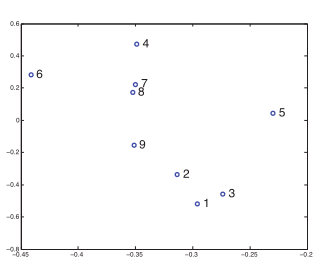
\includegraphics[width=0.4\linewidth]{fig/figure24}
	\caption*{图12.24: 将9份文件投影到二维。lsiCode生成的图。}
\end{figure}


\textbf{练习12.11} PPCA与FA

(来源:练习14.15(Hastie等人,2009),由Hinton提供。)。从以下模型中生成200个观察值,其中$\z_i \sim \mathcal{N}(\0,\I):x_{i1}=z_{i1},x_{i2}=z_{i1}+0.001z_{i2},x_{i3}=10z_{i3}$。拟合具有1个潜在因子的FA和PCA模型。因此表明,在主成分分析的情况下,相应的权重向量$\w$与最大方差方向(维数3)对齐,但在FA的情况下与最大相关方向(维数1+2)对齐。 


\clearpage
\section{稀疏线性模型 }
\subsection{介绍}
我们在第3.5.4节中介绍了特征选择的主题,其中我们讨论了寻找与输出具有高互信息的输入变量的方法。这种方法的问题在于,它基于一种短视的策略,一次只看一个变量。如果存在交互效应,则可能会失败。例如,如果$y=xor(x_1,x_2)$,那么$x_1$和$x_2$本身都不能预测响应,但它们一起可以完美地预测响应。关于这方面的真实例子,请考虑基因关联研究:有时两个基因本身可能是无害的,但当它们同时存在时,会导致隐性疾病(Balding 2006)。 

在本章中,我们重点关注使用基于模型的方法一次选择变量集。如果该模型是一个广义线性模型,对于某些链接函数f,其形式为$p(y|\x)=p(y|f(\w^T\x))$,那么我们可以通过鼓励权重向量$\w$是\textbf{稀疏}的来进行特征选择。即有大量的零。事实证明,这种方法具有显著的计算优势,我们将在下文中看到。 

以下是一些特征选择/稀疏性有用的应用程序: 
\begin{itemize}
\item 在许多问题中,我们有比训练案例N更多的维度D。相应的设计矩阵是短而胖的,而不是高而瘦的。这叫做\textbf{小N,大D问题}。随着我们开发更多的高通量测量设备,例如,利用基因微阵列,这变得越来越普遍,测量$D\sim 10000$个基因,但只得到$N\sim 100$个这样的例子。(这可能是即使是我们的数据似乎也在变得越来越胖的时代的一个迹象……)我们可能希望找到能够准确预测响应(例如细胞生长率)的最小特征集,以防止过度拟合,降低构建诊断设备的成本,或帮助科学洞察问题。 
\item  在第14章中,我们将使用以训练示例为中心的基函数,因此$\boldsymbol{\phi}(\x)=[\kappa (\x,\x_1),...,\kappa(\x,\x_N)]$,其中$\kappa$是一个核函数。得到的设计矩阵大小为$N\times N$。在这种情况下,特征选择相当于选择训练示例的子集,这有助于减少过拟合和计算成本。这被称为稀疏内核机器。 
\item 在信号处理中,通常用小波基函数表示信号(图像、语音等)。为了节省时间和空间,根据少量此类基函数找到信号的稀疏表示非常有用。这使我们能够从少量测量中估计信号,并对信号进行压缩。详见第13.8.3节。 
\end{itemize}

请注意,特征选择和稀疏性主题是当前机器学习/统计中最活跃的领域之一。在本章中,我们只剩下篇幅来概述主要结果。

\subsection{贝叶斯变量选择}
提出变量选择问题的自然方法如下。如果特征j“相关”,则设$\gamma_j=1$,否则设$\gamma_j=0$。我们的目标是计算后验模型 
\begin{equation}
	p(\gamma|\mathcal{D})=\dfrac{e^{-f(\gamma)}}{\sum\nolimits_{\gamma'}e^{-f(\gamma')}}\tag{13.1}
\end{equation}
其中$f(\gamma)$是成本函数: 
\begin{equation}
	f(\gamma)\triangleq -[\log p(\mathcal{D}|\gamma)+\log p(\gamma)]\tag{13.2}
\end{equation}
例如,假设我们从$D=10$维线性回归模型$y_i\sim \mathcal{N}(\w^T\x_i,\sigma^2)$中生成$N=20$个样本,其中,$\w$的$K=5$个元素为非零 。特别是,我们使用$\w=(0.00,-1.67, 0.13, 0.00, 0.00, 1.19, 0.00, -0.04,0.33,0.00)$和$\sigma^2=1$。我们列举了所有$2^{10}=1024$个模型,并计算每个模型的$p(\gamma|\mathcal{D})$(我们给出了下面的等式)。我们按格雷码顺序对模型进行排序,以确保连续向量恰好相差1位(原因是计算性的,在第13.2.3节中讨论)。 

结果位模式集如图13.1(a)所示。每个模型的成本$f(\gamma)$,如图13.1(b)所示。我们看到,这个目标函数非常“颠簸”。如果我们计算模型$p(\gamma|\mathcal{D})$上的后验分布,结果更容易解释。这如图13.1(c)所示。前8模型如下: 

\begin{center}
	\begin{tabular}{ccc}
	
	model & prob & member \\
	\midrule
	4 & 0.447 & 2,  \\
	61 & 0.241 & 2,6,  \\
	452 & 0.103 & 2,6,9,  \\
	60 & 0.091 & 2,3,6  \\
	29 & 0.041 & 2,5,  \\
	68 & 0.021 & 2,6,7,  \\
	36 & 0.015 & 2,5,6,  \\
	5 & 0.010 & 2,3,  \\
\end{tabular}
\end{center}

“真实”模型是$\{$2,3,6,8,9$\}$。然而,与特征3和8相关的系数非常小(相对于$\sigma^2$)。因此,这些变量更难检测。如果有足够的数据,该方法将收敛于真实模型(假设数据是从线性模型生成的),但对于有限的数据集,通常会存在相当大的后验不确定性。 

在大量模型上解释后验数据相当困难,因此我们将寻求各种汇总统计数据。自然模式是后验模式,或MAP估计
\begin{equation}
	\boldsymbol{\hat{\gamma}}=argmax(\boldsymbol{\gamma} | \mathcal{D})=argminf(\boldsymbol{\gamma})\tag{13.3}
\end{equation}

\begin{figure}[h]
	\centering
	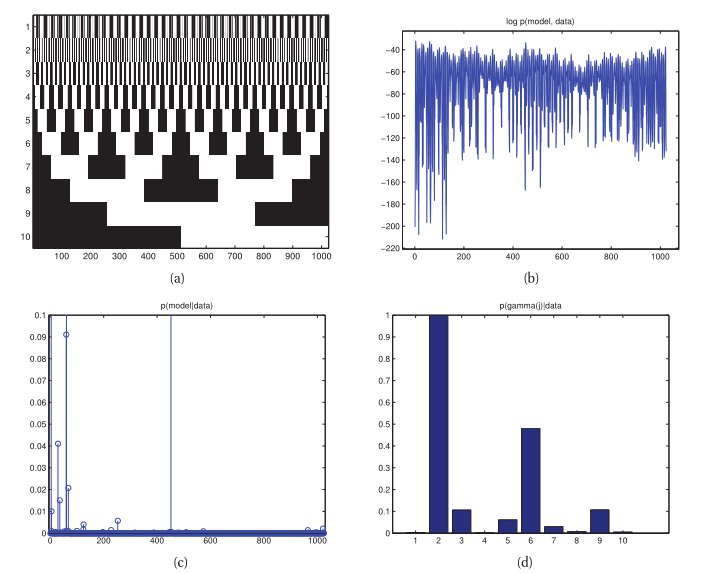
\includegraphics[width=0.7\linewidth]{fig13/figure1}
	\caption*{图13.1:(a)长度为10的所有可能位向量按格雷码顺序枚举。(b) 所有可能模型的评分函数。(c) 所有1024个模型的后验。为了清晰起见,垂直比例被截断为0.1。(d) 边际包容概率。图由linregAllsubsetsGraycodeDemo生成。}
\end{figure}
然而,该模式往往不能代表全部后部质量(见第5.2.1.3节)。一个更好的总结是\textbf{中值模型}(Barbieri and Berger 2004; Carvahlo and Lawrence 2007)。计算时使用
\begin{equation}
	\boldsymbol{\hat{\gamma}}=\{ j:p(\gamma_j=1|\mathcal{D})>0.5\}\tag{13.4}
\end{equation}
这需要计算后边缘包含概率$p(\gamma_j=1|\mathcal{D})$。如图13.1(d)所示。我们看到,该模型确信包含变量2和6;如果我们将决策阈值降低到0.1,我们还将添加3和9。然而,如果我们想要“捕获”变量8,我们将产生两个误报(5和7)。这种权衡第5.7.2.1节将更详细地讨论假阳性和假阴性之间的权衡。 

上面的例子说明了变量选择的“黄金标准”:问题足够小(只有10个变量),我们能够精确计算完整的后验值。当然,变量选择在维数较大的情况下最有用。由于存在$2^D$可能模型(位向量),因此通常不可能计算全后验概率,甚至难以找到总结,例如映射估计或边缘包含概率。因此,我们将在本章的大部分时间集中于算法加速。但是在我们这样做之前,我们将解释如何在上面的例子中计算$p(\gamma |\mathcal{D})$。 

\subsubsection{尖峰和板模型 }
后面的公式为: 
\begin{equation}
	p(\gamma |\mathcal{D})\varpropto p(\gamma )p(\mathcal{D}|\gamma )\tag{13.5}
\end{equation}

我们首先考虑先验,然后考虑可能性。 

通常在位向量上使用以下先验: 
\begin{equation}
	p(\gamma)=\prod_{j=1}^D Ber(\gamma_j|\pi_0)=\pi^{\parallel\gamma\parallel_0}(1-\pi_0)^{D-||\gamma||_0}\tag{13.6}
\end{equation}
其中,$\pi_0$是一个特征相关的概率,$||\gamma||_0=\sum\nolimits_{j=1}^D\gamma_j$是$\ell
_0$的\textbf{伪正态}。也就是向量中非零元素的数量。为了与后来的模型进行比较,将对数先验写成以下形式是很有用的为了与后面的模型相比较,把对数先验写成以下样子是很有用的。
\begin{align}
	\log p(\gamma|\pi_0)\ &=\ ||\gamma||_0\log \pi_0+(D-||\gamma ||_0)\log (1-\pi_0)\tag{13.7}\\
	&=\ ||\gamma ||_0(\log \pi_0-\log (1-\pi_0))+const\tag{13.8}\\
	&=\ -\lambda||\gamma ||_0+const\tag{13.9}
\end{align}
其中$\lambda\triangleq\log \dfrac{1-\pi_0}{\pi_0}$控制模型的稀疏性。 

我们可以把这个可能性写成如下:
\begin{equation}
	p(\mathcal{D}|\gamma )=p(\y|\X,\boldsymbol{\gamma } )=\iint p(\y|\X,\w,\boldsymbol{\gamma })p(\w|\gamma ,\sigma ^2)p(\sigma ^2)d\w d\sigma^2\tag{13.10}
\end{equation}

为了简化符号,我们假设响应居中(即$\overline{y}=0$),因此可以忽略任何偏移项$\mu$。 

我们现在讨论先验$p(\w|\gamma,\sigma^2)$。如果$\gamma_j=0$,特征j是无关的,因此我们期望$w_j=0$。如果$\gamma_j=1$,我们期望$w_j$是非零的。如果我们标准化输入,一个合理的先验是$\mathcal{N}(0,\sigma^2\sigma_w^2)$,其中$\sigma_w^2$控制我们预期与相关变量相关的系数的大小(由整体噪声级$\sigma^2$缩放)。我们可以总结如下: 

\begin{equation}
	p(w_j|\sigma^2,\gamma_j)=\left\{ 
	\begin{array}{ll}
	
	\delta_0(w_j) & \text{if } \gamma_j=0\\
	\mathcal{N}(w_j|0,\sigma^2\sigma_w^2) & \text{if } \gamma_j=1
	\end{array} \right. \tag{13.11}
\end{equation}
第一项是原点的“尖峰”。像$\sigma \to \infty$, 分布$p(w_j|\gamma_j=1)$接近均匀分布,可以将其视为恒定高度的“板”。因此,这被称为\textbf{钉板模型}(Mitchell和Beauchamp 1988)。

我们可以从模型中删除系数$w_j$,其中$w_j=0$,因为在先验条件下,它们被钳制为零。因此,等式13.10变为以下(假设高斯似然):
\begin{equation}
	p(\mathcal{D}|\gamma )=\iint \mathcal{N}(\y|\X_\gamma\w_\gamma,\sigma^2\I_N)\mathcal{N}(\w_\gamma|\0_{D_\gamma},\sigma^2\sigma_w^2\I_{D_\gamma})p(\sigma^2)d\w_\gamma d \sigma^2\tag{13.12}
\end{equation}

其中$D_\gamma=||\gamma||_0$是$\gamma$中非零元素的数量。在接下来的内容中,我们将通过定义任意正定矩阵$\textstyle{\sum\nolimits_{\gamma}}$ \footnote{通常使用$\sum\nolimits_{\gamma} g (\X_{\gamma}^T \X_{\gamma})^{-1}$形式的g先验第7.6.3.1节解释的原因(另见练习13.4)。已经提出了各种设置g的方法,包括交叉验证、经验贝叶斯(Minka 2000b;George和Foster 2000)、层次贝叶斯(Liang等人,2008)等。 }的形式$p(\w|\gamma,\sigma^2)=\mathcal{N}(\w_\gamma |\0_{D_\gamma},\sigma\boldsymbol{\textstyle{\sum\nolimits_{\gamma}}})$的先验来稍微概括这一点。

考虑到这些先验,我们现在可以计算边际似然。如果噪声方差已知,我们可以将边际似然(使用等式13.151)记下如下: 
\begin{align}
p(\mathcal{D}|\boldsymbol{\gamma}^2)\ \ &=\ \ \int \mathcal{N}(\y | \X_{\gamma} \w_{\gamma},\sigma^2\I)\mathcal{N}(\w_\gamma|\0,\sigma^2\textstyle\sum\nolimits_{\gamma})d\w_\gamma =\mathcal{N}(\y|\0,\C_\gamma)\tag{13.13}\\
\C_\gamma\ \ &\triangleq \ \ \sigma^2 \X_{\gamma}\textstyle\sum\nolimits_{\gamma}\X_{\gamma}^T+\sigma^2\I_N\tag{13.14}
\end{align}

如果噪声未知,我们可以对其进行先验分析并将其积分。通常使用$p(\sigma^2)=IG(\sigma^2|a_{\sigma},b_{\sigma})$关于设置a、b的一些指南见(Kohn等人,2001年)。如果我们使用$a=b=0$,我们恢复Jeffrey先验,$p(\sigma^2)\propto \sigma^{-2}$当我们积分出噪声时,我们得到以下更复杂的边际似然表达式(Brown等人,1998): 
\begin{align}
	p(\mathcal{D}|\gamma)\ \ &=\ \ \iint p(\y|\gamma,\w_\gamma ,\sigma^2)p(\w_\gamma|\gamma ,\sigma^2)p(\sigma^2)d\w_\gamma d\sigma^2\tag{13.15}\\
	&\propto\ \ |\X_\gamma^T\X_\gamma +\boldsymbol{\textstyle\sum}\nolimits_{\gamma}^{-1}|^{-\frac{1}{2}}|\boldsymbol{\textstyle\sum}\nolimits_{\gamma}|^{-\frac{1}{2}}(2b_\sigma+S(\gamma))^{-(2a_\sigma+N-1)/2}\tag{13.16}
\end{align}
其中$S(\gamma)$是RSS:
\begin{equation}
	S(\gamma)\ \ \triangleq\ \ \y^T\y-\y^T\X_\gamma(\X_\gamma^T\X_\gamma+\boldsymbol{\textstyle\sum}\nolimits_{\gamma}^{-1})^{-1}\X_\gamma^T\y\tag{13.17}
\end{equation} 
另见练习13.4。 

当无法以闭合形式计算边际似然时(例如,如果我们使用的是逻辑回归或非线性模型),我们可以使用具有以下形式的BIC进行近似 
\begin{equation}
	\log p(\mathcal{D}|\gamma)\approx \log p(\y|\X,\hat{\w}_\gamma,\hat{\sigma}^2)-\frac{||\gamma||_0}{0}\log N\tag{13.18}
\end{equation}
其中$\hat{\w}_\gamma$是基于$\X_\gamma$的ML或MAP估计,$||\gamma||_0$ 0是模型的“自由度”(Zou等人,2007)。加上对数先验,总体目标变成了
\begin{equation}
	\log p(\gamma|\mathcal{D})\approx \log p(\y|\X,\hat{\w}_\gamma,\hat{\sigma}^2)-\frac{||\gamma||_0}{0}\log N-\lambda||\gamma||_0+const\tag{13.19}
\end{equation}
我们看到有两个复杂度惩罚:一个来自BIC近似的边际似然,另一个来自$p(\gamma)$的先验。边际似然产生的,另一个是由$p(\gamma)$的先验产生的。很明显,这两个参数可以合并为一个整体的复杂性参数,我们用$\gamma$来表示。

\subsubsection{从伯努利-高斯模型到$\ell_0 $正则化}
有时使用的另一个模型(例如(Kuo和Mallick 1998;Zhou等人2009;Soussen等人2010))如下: 
\begin{align}
	y_i|\x_i,\w,\gamma,\sigma^2\ \ &\sim\ \ \mathcal{N}(\sum_{j}\gamma_jw_jx_{ij},\sigma^2)\tag{13.20}\\
	\gamma_j\ \ &\sim\ \ Ber(\pi_0)\tag{13.21}\\
	w_j\ \ &\sim\ \ \mathcal{N}(0,\sigma_w^2)\tag{13.22}
\end{align}
在信号处理文献中(例如(Soussen等人,2010)),这被称为\textbf{伯努利高斯}模型,尽管我们也可以称其为\textbf{二进制掩码}模型,因为我们可以将$\gamma_j$变量视为“掩盖”权重$w_j$。 

与尖峰和板模型不同,我们不整合“无关”系数;它们总是存在的。此外,二元掩码模型的形式为$\gamma_j\to \y \gets w_j$,而尖峰和平板模型的形式为$\gamma_j \to w_j \to \y$,在二元掩码模型中,只能从似然中识别乘积$\gamma_jw_j$。 

该模型的一个有趣方面是,它可以用于推导在(非贝叶斯)子集选择文献中广泛使用的目标函数。首先,注意联合先验具有以下形式: 
\begin{equation}
	p(\gamma,\w)\propto \mathcal{N}(\w|\0,\sigma_w^2\I)\pi_0^{||\gamma||_0}(1-\pi_0)^{D-||\gamma||_0}\tag{13.23}
\end{equation}
因此,缩放后的非正态化负对数后验的形式为: 
\begin{align}
	f(\gamma,\w)\ \ \triangleq\ \ &-2\sigma^2\log p(\gamma,\w,\y|\X)=||\y-\X(\gamma.*\w)||^2\\
	&+\frac{\sigma^2}{\sigma_w^2}||\w||^2+\lambda||\gamma||_0+const\tag{13.24}
\end{align}
其中:
\begin{equation}
	\lambda\triangleq 2\sigma^2\log (\frac{1-\pi_0}{\pi_0})\tag{13.25}
\end{equation}
让我们把$\w$分成两个子向量,$\w_{-\gamma}$和$\w_\gamma$,分别由$\gamma$的零和非零项索引。因为$\X(\gamma.*\w)=\X_\gamma\w_\gamma$,我们可以设置$\w_{-\gamma}=0$. 

现在考虑$\sigma_w^2\to \infty$的情况, 因此,我们不正则化非零权重(因此没有来自边缘似然或其BIC近似的复杂度惩罚)。在这种情况下,目标变为 
\begin{equation}
	f(\gamma,\w)=||\y-\X_\gamma\w_\gamma||_2^2+\lambda||\gamma||_0\tag{13.26}
\end{equation}
这与上述BIC目标类似。 

我们可以将相关变量集定义为$\w$的支持集或非零项集,而不是跟踪位向量$\gamma$。然后我们可以将上述等式重写为: 
\begin{equation}
	f(\w)=||\y-\X\w||_2^2+\lambda||\w||_0\tag{13.27}
\end{equation}
这被称为\textbf{$\ell_0$正则化}。我们已经将离散的优化问题(对$\gamma\in \{0,1\}^D$转化为连续问题(在$\w\in \mathbb{R}^D$上);然而$\ell_0$伪规范使目标非常不平滑。目标非常不平滑,所以这仍然很难优化。我们将在本章后面讨论不同的解决方案我们将在本章的其余部分讨论不同的解决方案。

\subsubsection{算法}
由于存在$2^D$模型,我们无法探索全后验,也无法找到全局最优模型。相反,我们将不得不求助于某种形式的启发式。我们将讨论的所有方法都涉及在模型空间中搜索,并评估每个点的成本$f(\gamma)$。这需要在每一步拟合模型(即计算$argmax\ p(\mathcal{D}|\w)$或评估其边际似然(即计算$\int p(\mathcal{D}|\w)p(\w)d\w$)这有时被称为\textbf{封装方法},因为我们将搜索最佳模型(或一组好模型)“包装”在通用模型拟合过程周围。 

\begin{figure}[h]
	\centering
	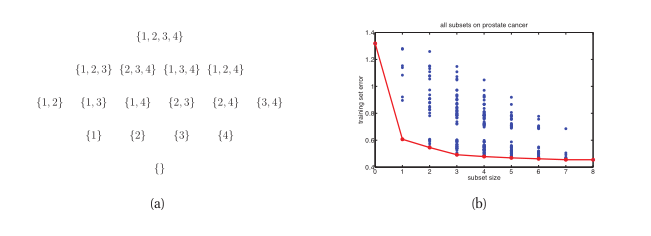
\includegraphics[width=0.9\linewidth]{fig13/figure2}
	\caption*{图13.2: (a) {1, 2, 3, 4}的子集网格。(b) 残余平方和与子集大小的关系,在
		前列腺癌数据集。下方的包络是任何给定大小的集合所能达到的最佳RSS。基于
		(Hastie et al. 2001)的图3.5。图由prostateSubsets生成。}
\end{figure}
为了使包装方法有效,重要的是我们可以快速评估一些新模型的得分函数,$\gamma'$,考虑到先前模型的分数,$\gamma$。只要我们能够有效地更新计算$f(\gamma)$所需的足够统计信息,就可以做到这一点。如果$\gamma'$仅在一位上与$\gamma$不同(对应于添加或删除单个变量),并且假设$f(\gamma)$仅取决于通过$\X_\gamma$的数据。在这种情况下,我们可以使用秩一矩阵更新/下降来有效地计算$\X_{\gamma'}^T\X_\gamma$来自$\X_{\gamma}^T\X_\gamma$。这些更新通常应用于$\X$的QR分解。有关详细信息,请参见(Miller 2002;Schniter等人,2008)。 

\subsubsection*{13.2.3.1 贪婪搜索 }
假设我们想要找到地图模型。如果我们使用$\ell_0$-正则化目标在等式13.27中,我们可以利用最小二乘法的性质来推导各种有效的贪心正向搜索方法,其中一些我们总结如下。有关更多详细信息,请参见(Miller 2002;Soussen等人,2010)。 
\begin{itemize}
\item \textbf{单一最佳替换}最简单的方法是使用贪心爬山,在每个步骤中,我们将当前模型的邻域定义为通过翻转一位$\gamma$可以达到的所有模型,即,对于每个变量,如果它当前不在模型中,我们考虑添加它,如果它当前在模型中,我们考虑删除它。在(Soussen等人,2010年)中,他们将其称为单一最佳替换(SBR)。由于我们希望得到稀疏解,我们可以从空集$\gamma=\0$开始。我们基本上是在子集的晶格中移动,如图13.2(a)所示。我们继续添加或删除,直到无法改善为止。 
\item \textbf{正交最小二乘法}如果我们在等式13.27中设置$\gamma=0$,那么没有复杂度惩罚,就没有理由执行删除步骤。在这种情况下,SBR算法等效于\textbf{正交最小二乘法}(Chen和Wigger 1995),而正交最小二乘法又等效于贪婪\textbf{正向选择}。 在该算法中,我们从空集开始,在每一步添加最佳特征。误差将随着$||\gamma||_0$单调下降,如图13.2(b)所示。我们可以选择下一个最好的功能$j^*$通过求解将$\gamma_t$添加到当前集合
\begin{equation}
	j^*=arg\ \min_{j\notin \gamma_t}\min_\w||\y-(\X_{\gamma_t\cup j})\w||^2\tag{13.28}
\end{equation}
然后,我们通过设置$\gamma^{(t+1)}=\gamma^{(t)}\cup \{j^*\}$来更新活动集. 为了选择下一个要在步骤t中添加的特征,我们需要求解第t步的$D-D_t$最小二乘问题,其中$D_t=|\gamma_t|$是当前活动集的基数。选择了要添加的最佳特征后,我们需要解决一个额外的最小二乘问题来计算$\w_{t+1}$)。 
\item \textbf{正交匹配追求}正交最小二乘有点昂贵。一种简化方法是将当前权重“冻结”为其当前值,然后通过求解选择下一个要添加的特征 
\begin{equation}
	j^*=arg\ \min_{j\notin \gamma_t}\min_\beta||\y-\X\w_t-\beta\x_{:,j}||^2\tag{13.29}
\end{equation}
这种内部优化很容易求解:我们只需设置$\beta =\x_{:,j}^T\r_t/||\x_{:,j}||^2$其中$\r_t=\y-\X\w_t$是当前残差向量。如果列是单位范数,我们有 
\begin{equation}
	j^*=arg\ max\x_{:,j}^T\r_t\tag{13.30}
\end{equation}
所以我们只是寻找与当前残差最相关的列。然后,我们更新活动集,并使用$\X_{\gamma_{t+1}}$计算新的最小二乘估计$\w_{t+1}$。这种方法称为\textbf{正交匹配追踪或OMP}(Mallat等人,1994)。每次迭代只需要一次最小二乘计算,因此比正交最小二乘法更快,但不太准确(Blumensath和Davies 2007)。
\item \textbf{匹配追求}更激进的近似方法是贪婪地添加与当前残差最相关的特征。这被称为\textbf{匹配追求}(Mallat和Zhang 1993)。这也相当于一种称为最小二乘增压的方法(第16.4.6节)。
\item \textbf{向后选择}向后选择从模型中的所有变量(所谓的\textbf{饱和模型})开始,然后在每一步删除最差的变量。这相当于从晶格顶部向下执行贪婪搜索。这比自底向上搜索可以得到更好的结果,因为关于是否保留变量的决定是在可能依赖于它的所有其他变量的上下文中作出的。然而,这种方法通常不适用于大型问题,因为饱和模型的拟合成本太高。 
\item \textbf{FoBa}(Zhang 2008)的\textbf{前后向算法}与上述单一最佳替换算法类似,只是在选择下一步时使用了类似OMP的近似值。(Moghaddam等人,2008年)中描述了类似的“双通道”算法。
\item \textbf{贝叶斯匹配追踪}(Schniter等人,2008年)的算法与OMP相似,只是它使用贝叶斯边际似然评分标准(在尖峰和平板模型下)而不是最小二乘目标。此外,它使用波束搜索的形式一次探索穿过晶格的多条路径。 
\end{itemize}

\subsubsection*{13.2.3.2   随机搜索 }
如果我们想要近似后验概率,而不仅仅是计算模式(例如,因为我们想要计算边缘包含概率),一种选择是使用多通道蒙特卡洛方法。标准方法是使用Metropolis Hastings,其中提案分发仅翻转单个位。这使我们能够有效地计算给定$p(\gamma'|\mathcal{D})$的$p(\gamma|\mathcal{D})$。通过计算随机游动访问该状态的次数来估计状态(位配置)的概率。有关此类方法的综述,请参见(O'Hara和Sillanpaa 2009),以及(Bottolo和Richardson 2010),了解基于进化MCMC的最新方法。 

然而,在离散状态空间中,多通道蒙特卡洛方法不必要地低效,因为我们可以直接使用$p(\gamma,\mathcal{D})=exp(-f(\gamma))$来计算状态的(非规范化)概率;因此,没有必要再次访问一个国家。一种更有效的替代方法是使用某种随机搜索算法,生成一组高分模型,然后进行以下近似 
\begin{equation}
	p(\gamma|\mathcal{D})\approx \dfrac{e^{-f(\gamma)}}{\sum\nolimits_{\gamma'\in S}e^{-f(\gamma')}}\tag{13.31}
\end{equation}
请参阅(Heaton和Scott,2009年),了解此类最新方法的综述。 

\subsubsection*{13.2.3.3  EM与变分推理* }
很容易将EM应用于尖峰和平板模型,其形式为$\gamma_j\to w_j\to \y$,我们可以在E步中计算$p(\gamma_j=1|w_j)$,并在M步中优化$\w$。然而,这是行不通的,因为当我们计算$p(\gamma_j=1|w_j)$时,我们比较了$\delta$函数$\delta_0(w_j)$和高斯pdf,$\mathcal{N}(w_j|0,\sigma_w^2)$ 。我们可以用窄的高斯函数代替$\delta$函数,然后E步相当于在两种可能的高斯模型下对$w_j$进行分类。然而,这可能会受到严重的局部极小值的影响。 

另一种方法是将EM应用于伯努利-高斯模型,其形式为$\gamma_j\to \y \gets w_j$。在这种情况下,后验$p(\gamma|\mathcal{D},\w)$难以计算,因为所有位由于解释而变得相关。然而,可以导出形式为$\prod_jq(\gamma_j)q(w_j)$的平均场近似(Huang等人,2007;Rattray等人,2009)。 

\subsection{$\ell_1$正则化:基础知识}
当我们有许多变量时,计算上很难找到$p(\gamma|\mathcal{D})$的后验模式。虽然贪婪算法通常工作良好(参见zhang2008的理论分析),但它们当然会陷入局部最优。

部分问题是由于$\gamma_j$变量是离散的,$\gamma_j\in \{0,1\}$。在优化领域,通常通过用连续变量替换离散变量来放松这种形式的硬约束。我们可以通过替换尖峰和板状先验来实现这一点,尖峰和板状先验将有限概率质量分配给$w_j=0$的事件,并通过在原点附近放置大量概率密度来“鼓励”$w_j=0$的连续先验,例如零平均拉普拉斯分布。这在第7.4节稳健线性回归的背景下首次介绍。在那里,我们利用了拉普拉斯有重尾巴的事实。在这里,我们利用了它在$\mu=0$附近有一个尖峰的事实。更准确地说,考虑该形式的先验
\begin{equation}
	p(\w|\lambda)=\prod_{j=1}^DLap(w_j|0,1/\lambda)\propto \prod_{j=1}^De^{-\lambda|w_j|}\tag{13.32}
\end{equation}

\begin{figure}[h]
	\centering
	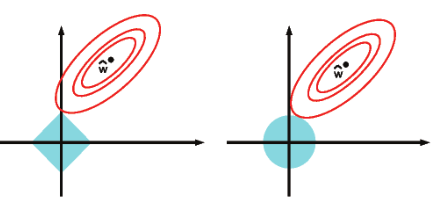
\includegraphics[width=0.7\linewidth]{fig13/figure3}
	\caption*{图13.3:演示最小二乘问题的$\ell_1$(左)和$\ell_2$(右)正则化。根据(Hastie等人,2001年)的图3.12。}
\end{figure}
我们将使用一个关于偏移项的统一先验,$p(w_0)\propto 1$。让我们用这个先验来进行MAP估计。
这个先验。惩罚性负对数似然有如下形式
\begin{equation}
	f(\w)=-\log p(\mathcal{D}|\w)-\log p(\w|\lambda)=NLL(\w)+\lambda||\w||_1\tag{13.33}
\end{equation}
其中$||\w||_1=\sum\nolimits_{j=1}^D|w_j|$是$\w$的$\ell_1$范数。对于适当大的$\lambda$,估计$\hat{\w}$将是稀疏的,原因我们解释如下。事实上,这可以被认为是非凸的凸近似$\ell_0$目标
\begin{equation}
	\argmin_\w NLL(\w)+\lambda||\w||_0\tag{13.34}
\end{equation}
在线性回归的情况下$\ell_1$目标变成
\begin{align}
	f(\w)\ \ &=\ \ \sum_{i=1}^{N}-\frac{1}{2\sigma^2}(y_i-(w_0+\w^T\x_i))^2+\lambda||\w||_1\tag{13.35}\\
	&=\ \ RSS(\w)+\lambda'||\w||_1\tag{13.36}
\end{align}
其中$\lambda'=2\lambda\sigma^2$。这种方法称为\textbf{基追踪去噪或BPDN}(Chen等人,1998)。这个术语的原因将在后面变得清晰。一般来说,将零均值的拉普拉斯先验放在参数上的技术拉普拉斯先验参数并进行MAP估计的技术被称为正则化。它可以与任何凸的或非凸的NLL项相结合。许多不同的算法我们在第13.4节中对其中的一些算法进行了回顾。

\subsubsection{为什么$\ell_1$正则化产生稀疏解?}
我们现在解释为什么$\ell_1$正则化导致稀疏解,然而$\ell_2$正则化不适用。我们关注线性回归的情况,尽管类似的论点适用于逻辑回归和其他GLM。

目标是以下非光滑目标函数:
\begin{equation}
	\min_\w RSS(\w)+\lambda||\w||_1\tag{13.37}
\end{equation}
我们可以将其改写为约束但平滑的目标(具有线性约束的二次函数):
\begin{equation}
\min_\w RSS(\w)\ \ \ s.t.\ \ \ ||\w||_1\le B\tag{13.38}
\end{equation}
其中,B是权重$\ell_1$范数的上界:小(紧)界B对应于大惩罚$\lambda$,反之亦然。\footnote{等式13.38是\textbf{二次规划或QP}的示例,因为我们有一个受线性不等式约束的二次目标。其拉格朗日由等式13.37给出。}等式13.38被称为\textbf{lasso},代表“最小绝对收缩和选择算子”(Tibshirani 1996)。我们稍后将了解它为什么有这个名称。

类似地,我们可以写成岭回归
\begin{equation}
	\min_\w RSS(\w)+\lambda||\w||_2^2\tag{13.39}
\end{equation}

或作为绑定约束形式:
\begin{equation}
\min_\w RSS(\w)\ \ \ s.t.\ \ \ ||\w||_2^2\le B\tag{13.40}
\end{equation}

在图13.3中,我们绘制了RSS目标函数的轮廓,以及$\ell_2$和$\ell_1$约束曲面。根据约束优化理论,我们知道最优解发生在目标函数的最低水平集与约束曲面相交的点(假设约束是活动的)。几何上应该很清楚,当我们放松约束B时,我们“成长”$\ell_1$“球”,直到它达到目标;球的角比边更可能与椭圆相交,尤其是在高维情况下,因为角“突出”更多。角点对应于位于坐标轴上的稀疏解。相比之下,当我们成长的时候$\ell_2$球,它可以在任何点与目标相交;没有“角”,因此不喜欢稀疏性。

为了避免这种情况,请注意,对于岭回归,稀疏解的先验成本(如$\w=(1,0)$与稠密解的成本(如$\w=(1/\sqrt{2},1/\sqrt{2})$相同,只要他们有相同的$\ell_2$规范:
\begin{equation}
	||(1,0)||_2=||(1/\sqrt{2},1/\sqrt{2})||_2=1\tag{13.41}
\end{equation}
然而,对于lasso,设置$\w=(1,0)$比设置$\w=(1/\sqrt{2},1/\sqrt{2})$便宜,因此
\begin{equation}
||(1,0)||_1=1< ||(1/\sqrt{2},1/\sqrt{2})||_1=\sqrt{2}\tag{13.42}
\end{equation}
查看$\ell_1$正则化导致稀疏解的最严格方法是检查保持在最佳状态的条件。我们在第13.3.2节中这样做。

\subsubsection{lasso的最优性条件}
lasso目标的形式是
\begin{equation}
	f(\boldsymbol{\theta})=RSS(\boldsymbol{\theta})+\lambda||\w||_1\tag{13.43}
\end{equation}

\begin{figure}[h]
	\centering
	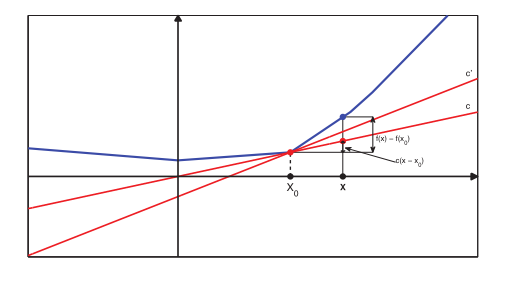
\includegraphics[width=0.7\linewidth]{fig13/figure4}
	\caption*{图13.4: 基于http://en.wikipedia.org/wiki/Subderivative上的图,对点x0处函数的一次导数进行了说明。由subgradientPlot生成的图形。}
\end{figure}

不幸的是,当$w_j=0$时,$||\w||_1$项不可微。这是一个\textbf{非光滑}优化问题的示例。

为了处理非光滑函数,我们需要扩展导数的概念。我们定义(凸)函数$f:\mathit{I}\to \mathbb{R}$在$\theta_0$点的\textbf{次导数或次梯度}为标量g,使得
\begin{equation}
	f(\theta)-f(\theta_0)\ge g(\theta-\theta_0)\ \forall\theta \in \mathit{I}\tag{13.44}
\end{equation}
其中$\I$是包含$\theta_0$的某个区间。见图13.4。\footnote{一般来说,对于一个矢量函数,如果对于所有矢量$\boldsymbol{\theta}$,我们说g是f在$\boldsymbol{\theta}_0$处的子梯度。
\begin{equation}
	f(\boldsymbol{\theta})-f(\boldsymbol{\theta}_0)\ge (\boldsymbol{\theta}-\boldsymbol{\theta}_0)^T\g\tag{13.45}
\end{equation}
 
 因此g是$\boldsymbol{\theta}_0$处函数的线性下界。}我们将子导数集定义为区间[a,b],其中a和b是单侧极限

\begin{equation}
	a=\lim\limits_{\theta\to \theta_0^-} \dfrac{f(\theta)-f(\theta_0)}{\theta-\theta_0},b=\lim\limits_{\theta\to \theta_0^+} \dfrac{f(\theta)-f(\theta_0)}{\theta-\theta_0}\tag{13.46}
\end{equation}
所有子导数的集合[a,b]称为函数f在$\theta_0$处的\textbf{次微分},并表示为$\partial
f(\theta)|_{\theta_0}$。例如,在绝对值函数$f(\theta)=|\theta|$的情况下,次导数由以下公式得出:
\begin{equation}
	\partial f(\theta)=
	\left\{
	\begin{array}{rl}
	\{-1\}& \ \ if\ \theta<0\\
	\left[-1,1\right]&\ \ if\ \theta = 0 \\
	\{+1\}&\ \ if\ \theta>0\tag{13.47}
	\end{array} \right.
\end{equation}
如果函数处处可微,那么$\partial f(\theta )=\{\frac{df(\theta)}{d\theta}\}$。通过类比标准微积分结果,可以证明点$\hat{\theta}$是f iff 0$\in \partial f(\theta)|\hat{\theta}$的局部极小值。
\begin{figure}[h]
	\centering
	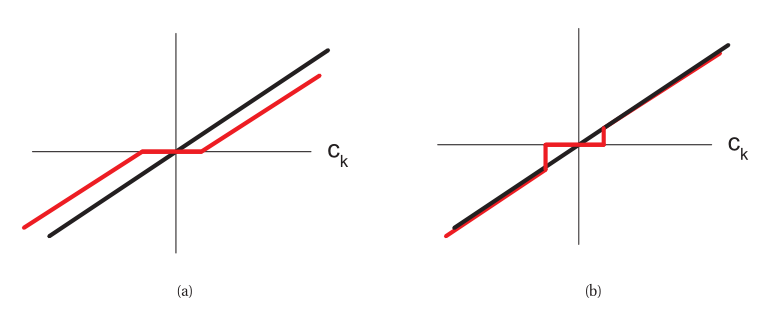
\includegraphics[width=0.7\linewidth]{fig13/figure5}
	\caption*{图13.5: 左图:软阈值处理。平坦区域是区间$[-\lambda, +\lambda]$。右图:硬阈值处理。}
\end{figure}

让我们将这些概念应用于lasso问题。让我们先忽略非光滑惩罚项。可以证明(练习13.1)
\begin{align}
	\frac{\partial}{\partial w_j}RSS(\w)\ &=\ a_jw_j-c_j\tag{13.48}\\
	a_j\ &=\ 2\sum_{i=1}^{n}x_{ij}^2\tag{13.49}\\
	c_j\ &=\ 2\sum_{i=1}^{n} x_{ij}(y_i-\w_{-j}^T\x_{i,-j})\tag{13.50}
\end{align}
其中$\w_{-j}$是不含分量j的$\w$,类似地,对于$\x_{i,-j}$,我们看到,$c_j$与第j个特征$\x$,j和其他特征$\r_{-j}=\y-\X_{:,-j}\w_{-j}$的残差之间的相关性(成比例),因此,$c_j$的幅值指示了特征j预测$\y$的相关程度(相对于其他特征和当前参数)。

加上惩罚项,我们发现次导数由以下公式得出:
\begin{align}
	\partial_{w_j}f(\w)\ &=\ (a_j w_j-c_j)+\lambda\partial_{w_j}||\w||_1\tag{13.51}\\
	&=\left\{\begin{array}{rl}
	\{a_jw_j-c_j-\lambda\}& \ \ \textbf{if}\ w_j<0\\
	\left[-c_j-\lambda,-c_j+\lambda \right]&\ \ \textbf{if}\ w_j = 0 \\
	\{a_j w_j-c_j-\lambda\}&\ \ \textbf{if}\ w_j>0\tag{13.52}
	\end{array} \right. 
\end{align}
我们可以用一种更紧凑的方式来写,如下所示:
\begin{equation}
	\X^T(\X \w- \y)_j\in \left\{\begin{array}{rl}
		\{-\lambda\}& \ \ \textbf{if}\ w_j<0\\
	\left[-\lambda,\lambda \right]&\ \ \textbf{if}\ w_j = 0 \\
	\{\lambda\}&\ \ \textbf{if}\ w_j>0\tag{13.53}
	\end{array} \right. 
\end{equation}

根据$c_j$的值,$\partial _{w_j}f(\w)=0$的解可能出现在3个不同的值上$w_j$的不同值,如下所示:
\begin{itemize}
\item[1.] 如果$c_j<-\lambda$,因此,特征与残差呈强负相关,则次梯度在$\hat{w}_j=\frac{c_j+\lambda}{a_j}<0$时为零。
\item[2.]
如果$c_j\in [-\lambda,\lambda]$,因此特征仅与残差弱相关,则次梯度在$\hat{w}_j=0$时为零。
\item[3.]
如果$c_j>\lambda$,则特征与残差呈强正相关,则次梯度在$\hat{w}_j=\frac{c_j-\lambda}{a_j}>0$处为零。
\end{itemize}

总之,我们有
\begin{equation}
	\hat{w}_j(c_j)=\left\{
	\begin{array}{cl}
	(c_j+\lambda)/a_j\ \ &if\  c_j<-\lambda\\
	0&if\  c_j\in [-\lambda,\lambda]\\
	(c_j-\lambda)/a_j\ \ &if\  c_j>\lambda
	\end{array} \right.\tag{13.54}
\end{equation}
我们可以这样写:
\begin{equation}
	\hat{w}_j=soft(\frac{c_j}{a_j};\frac{\lambda}{a_j})\tag{13.55}
\end{equation}
其中
\begin{equation}
	soft(a;\delta)\ \ \triangleq\ \ sign(a)(|a|-\delta)_+\tag{13.56}
\end{equation}

$x_+=max(x,0)$是x的正部分。这称为\textbf{软阈值}。这如图13.5(a)所示,其中我们绘制了$\hat{w}_j$与$c_j$。虚线是对应于最小二乘拟合的线$w_j=c_j/a_j$。实线表示正则化估计$\hat{w}_j(c_j)$,将虚线向下(或向上)移动$\lambda$,除非$-\lambda\le c_j\le \lambda$,在这种情况下,它将设置为$w_j=0$。

相比之下,在图13.5(b)中,我们说明了\textbf{硬阈值}。这将$w_j$的值设置为$-\lambda\le c_j\le \lambda$,但它不会将$w_j$的值收缩到该区间之外。软阈值线的斜率与对角线不重合,这意味着即使较大的系数也会向零收缩;因此,lasso是一种有偏估计。这是不可取的,因为如果可能性(通过$c_j$)表明系数$w_j$应该很大,我们不想缩小它。我们将在第13.6.2节中更详细地讨论这个问题。

现在我们终于可以理解为什么Tibshirani在(Tibshirani1996)中发明了术语“lasso”:它代表“最小绝对选择和收缩算子”,因为它选择变量的子集,并通过惩罚绝对值来收缩所有系数。如果$\lambda=0$,我们得到OLS解(最小$\ell_1$范数)。如果$\lambda\ge \lambda_{max}$,我们得到$\hat{\w}=0$,其中
\begin{equation}
	\lambda_{max}=||\X^T\y||_\infty=\max_j|\y^T\x_{;,j}|\tag{13.57}
\end{equation}

这个值是利用这样一个事实来计算的:如果$(\X^T\y)_j\in [-\lambda,\lambda]$,对所有j来说,$\0$是最优的。$\ell_1$正则化目标的最大惩罚是
\begin{equation}
	\lambda_{max}=\max_j|\nabla_jNLL(\0)|\tag{13.58}
\end{equation}

\subsubsection{最小二乘法、lasso、山脊法和子集选择法的比较}
通过将$\ell_1$正则化与最小二乘法进行比较,我们可以进一步了解$\ell_1$正则化,以及$\ell_2$和$\ell_0$正则化最小二乘。为了简单起见,假设$\X$的所有特征都是正交的,因此$\X^T\X=\I$。在这种情况下,RSS由以下公式得出:
\begin{align}
	RSS(\w)&=||\y-\X\w||^2=\y^T\y+\w^T\X^T\X\w-2\w^T\X^T\y\tag{13.59}\\
	&=const+\sum_{k}w_k^2-2\sum_{k}\sum_{i}w_kx_{ik}y_i\tag{13.60}
\end{align}

我们看到它分解成一个项的总和,每个维度一个。因此,我们可以分析地写下MAP和ML估计,如下所示:
\begin{itemize}
\item \textbf{极大似然估计}OLS解由以下公式得出:
\begin{equation}
	\hat{w}_k^{OLS}=\x_{:k}^T\y\tag{13.61}
\end{equation}
其中,$\x_{:k}$是$\X$的第k列。这与等式13.60非常相似。我们可以看到$\hat{w}_k^{OLS}$只是特征k在响应向量上的正交投影(见第7.3.2节)。
\item \textbf{Ridge} 人们可以证明,Ridge的估计值是由以下公式给出的
\begin{equation}
	\hat{w}_k^{ridge}=\frac{\hat{w}_k^{OLS}}{1+\lambda}\tag{13.62}
\end{equation}
\item \textbf{Lasso}来自等式13.55,利用$a_k=2$和$\hat{w}_k^{OLS}=c_k/2$的事实,我们得到
\begin{equation}
	\hat{w}_k^{lasso}=sign(\hat{w}_k^{OLS})(|\hat{w}_k^{OLS}|-\frac{\lambda}{2})_+\tag{13.63}
\end{equation}
这对应于软阈值,如图13.5(a)所示。
\item \textbf{子集选择}如果我们使用子集选择选择最佳K个特征,参数估计如下
\begin{equation}
	\hat{w}_k^{SS}=\left\{
	\begin{array}{cl}
	\hat{w}_k^{OLS} &\ \ if\ rank(|\hat{w}_k^{OLS}|)\le K\\
	0&\ \ othersize\tag{13.64}
	\end{array}
	\right.
\end{equation}
其中秩是指权重大小排序列表中的位置。这对应于硬阈值,如图13.5(b)所示。
\end{itemize}

图13.6(a)绘制了14次多项式lasso的均方误差与$\lambda$的关系,图13.6(b)绘制了均方误差与多项式阶数的关系。我们看到,lasso给出了与子集选择方法类似的结果。

再举一个例子,考虑一个关于前列腺癌的数据集。我们有$D=8$个特征和$N=67$个训练案例;目的是预测对数前列腺特异性抗原水平(更多生物学细节见(Hastie等人,2009年,p4))。表13.1表明,lasso比最小二乘法、岭回归和最佳子集回归具有更好的预测精度(至少在这个特定数据集上)。(在每种情况下,正则化器的强度都是通过交叉验证来选择的。)Lasso还产生了稀疏解。当然,对于其他问题,岭可能提供更好的预测准确性。实际上,lasso和脊的组合,即弹性网,通常表现最好,因为它提供了稀疏性和正则化的良好组合(见第13.5.3节)。

\begin{figure}[h]
	\centering
	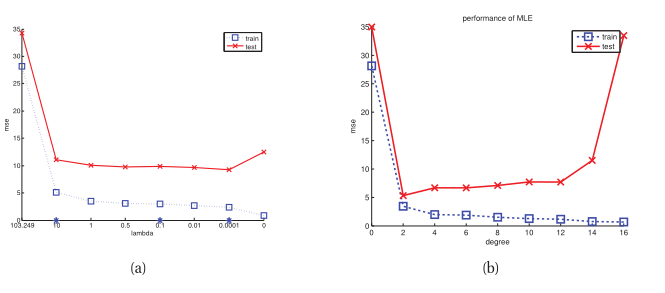
\includegraphics[width=0.7\linewidth]{fig13/figure6}
	\caption*{图13.6:(a)14次多项式的lasso的MSE与$\lambda$。注意,当我们向右移动时,$\lambda$减小。由linregPolyLassoDemo生成的图。(b) MSE与多项式次数。请注意,模型阶数随着向右移动而增加。一些多项式回归模型的曲线图见图1.18。由linregPolyVsDegree生成的图。}
\end{figure}

\begin{figure}[h]
	\centering
	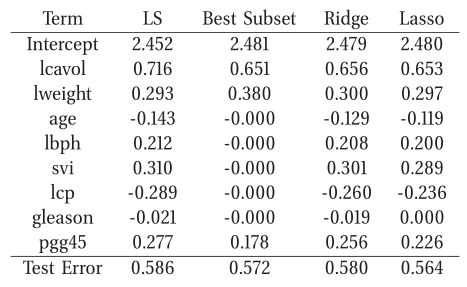
\includegraphics[width=0.7\linewidth]{fig13/table1}
	\caption*{表13.1: 不同方法对前列腺癌数据的结果,其中有8个特征和67个训练案例。方法有:最小二乘法,子集=最佳子集回归,岭,套索。行表示系数;我们看到子集回归和套索给出了稀疏解。底行是测试集的均方误差(30例)。根据(Hastie等人,2009年)的表3.3。通过前列腺比较生成的图。}
\end{figure}

\subsubsection{正则化路径}
随着$\lambda$的增加,解向量$\hat{\w}(\lambda)$将趋于稀疏,尽管不一定单调。我们可以绘制每个特征j的值$\hat{w}_j(\lambda)$与$\lambda$;这被称为正则化路径。

图13.7(a)中对ridge回归进行了说明,其中我们绘制了$\hat{w}_j(\lambda)$随正则化子$\lambda$减小的曲线。我们看到当$\lambda=\infty$, 所有系数均为零。但对于$\lambda$的任何有限值,所有系数都是非零的;此外,随着$\lambda$的减小,它们的幅值增大。

在图13.7(b)中,我们绘制了lasso的类似结果。当我们向右移动时,$\ell_1$惩罚的上限B增加。当$B=0$时,所有系数均为零。随着B的增加,系数逐渐“开启”。但对于0和$B_{max}=||\hat{\w}_{OLS}||_1$之间的任何值,解是稀疏的。\footnote{通常绘制与\textbf{收缩因子}(定义为$s(B)=B/B_{max}$的解,而不是与B的解。这仅影响水平轴的比例,而不影响曲线的形状。}

\begin{figure}[h]
	\centering
	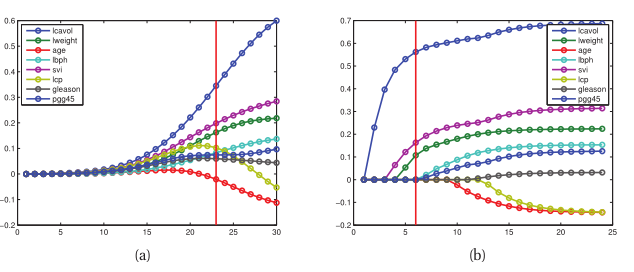
\includegraphics[width=0.7\linewidth]{fig13/figure7}
	\caption*{图13.7(a)前列腺癌示例与约束条件下的ridge系数曲线w的$\ell_2$范数,因此小t(大$\lambda$)在左侧。垂直线是使用1SE规则由5倍CV选择的值。根据(Hastie等人,2009年)的图3.8。由RidgePathProstation生成的图。(b) 前列腺癌的套索系数曲线示例与绑定w的$\ell_1$范数,因此小t(大$\lambda$)在左侧。根据(Hastie等人,2009年)的图3.10。图由LassopathProstation生成。}
\end{figure}

\begin{figure}[h]
	\centering
	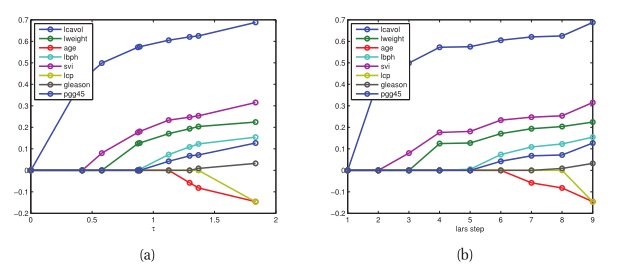
\includegraphics[width=0.7\linewidth]{fig13/figure8}
	\caption*{图13.8: 前列腺癌示例上lasso正则化路径的分段线性图示。(a) 对于B的临界值,我们绘制了$\hat{w}_j(B)$。(b)我们绘制了LARS算法的vs步长。图由LassopathProstation生成。}
\end{figure}

值得注意的是,可以证明解路径是B的分段线性函数(Efron等人,2004)。也就是说,存在一组B的临界值,其中非零系数的活动集发生变化。对于这些临界值之间的B值,每个非零系数以线性方式增加或减少。这如图13.8(a)所示。此外,可以解析求解这些临界值。这是\textbf{LARS}算法的基础(Efron等人,2004),该算法代表“最小角度回归和收缩”(详见第13.4.2节)。值得注意的是,LARS可以以与单个最小二乘拟合(即$O(min(ND^2,DN^2))$大致相同的计算成本计算整个正则化路径。

\begin{figure}[h]
	\centering
	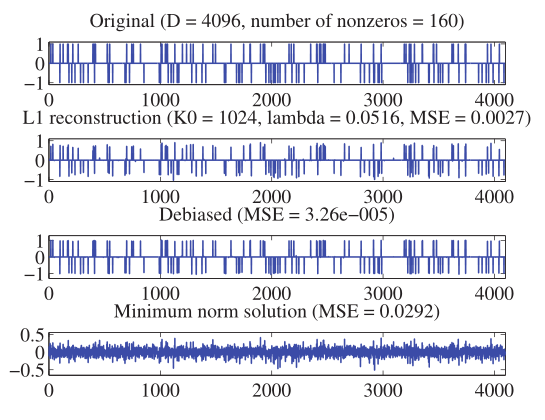
\includegraphics[width=0.7\linewidth]{fig13/figure9}
	\caption*{图13.9: 使用lasso恢复稀疏信号的示例。有关详细信息,请参阅文本。根据图1(Figueiredo等人,2007)。图由马里奥·菲盖雷多创作的sparseSensingDemo生成。}
\end{figure}

在图13.8(b)中,我们绘制了在B的每个临界值处计算的系数。现在分段线性更为明显。下面我们显示了沿正则化路径每一步的实际系数值(最后一行是最小二乘解):

\begin{figure}[h]
	\centering
	\caption*{清单13.1: LassopathProstation的输出}
	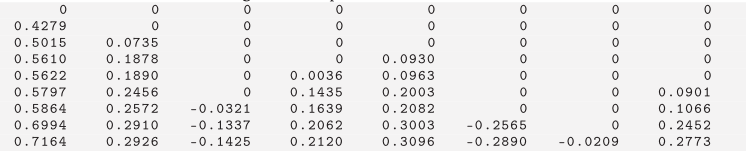
\includegraphics[width=0.7\linewidth]{fig13/list1}
\end{figure}

通过将B从0更改为$B_{max}$,我们可以从所有权重均为零的解转换为所有权重均为非零的解。不幸的是,并非所有子集大小都可以使用lasso实现。可以证明,如果$D>N$,最优解在达到对应于最小的OLS解的完整集之前,最多可以包含N个变量$\ell_1$标准。在第13.5.3节中,我们将通过使用$\ell_2$正则化子以及$\ell_1$正则化(一种称为弹性网的方法),我们可以获得比训练情况包含更多变量的稀疏解。这使我们能够探索N和D之间的模型尺寸。
\clearpage
\subsubsection{模型选择}
很容易使用$\ell_1$正则化来估计相关变量集。在某些情况下,我们可以恢复$\w^*$的真实稀疏模式, 生成数据的参数向量。一种可以在$N\to \infty$中恢复真实模型的方法称为\textbf{模型选择一致}。关于哪些方法以及何时享受该属性的细节超出了本书的范围;详见(Buhlmann和van de Geer 2011)。

我们将只展示一个小例子,而不是进行理论讨论。我们首先生成一个稀疏信号$\w^*$尺寸D=4096,由160个随机放置的$\pm 1$个尖峰组成。接下来,我们生成一个大小为$N\times D$的随机设计矩阵$\X$,其中N=1024。最后,我们生成一个噪声观测$\y=\X\w^*+\boldsymbol{\epsilon}$,其中$\epsilon_i\sim \mathcal{N}(0,0.01^2)$。然后我们根据$\y$和$\X$估计$\w$。

原始$\w^*$如图13.9的第一行所示。第二行是$\ell_1$使用$\lambda=0.1\lambda_{max}$估计$\hat{\w}_{L1}$。我们看到在正确的地方有“尖峰”,但它们太小了。第三行是基于supp($\hat{\w}_{L1}$)估计为非零的系数的最小二乘估计。这被称为\textbf{debiasing},并且是必要的,因为lasso收缩了相关系数以及不相关的系数。最后一行是所有系数的联合最小二乘估计,忽略稀疏性。我们看到,(基于debiased的)稀疏估计是对原始信号的一种很好的估计。相比之下,没有稀疏性假设的最小二乘法性能很差。

当然,要进行模型选择,我们必须选择$\lambda$。通常使用交叉验证。然而,需要注意的是,交叉验证是选择$\lambda$值,从而获得良好的预测精度。这通常与可能恢复“真实”模型的值不同。想知道为什么吗,记得$\ell_1$正则化执行选择和收缩,也就是说,所选系数更接近0。为了防止相关系数以这种方式收缩,交叉验证将倾向于选择一个不太大的$\lambda$值。当然,这将导致包含不相关变量(误报)的较稀疏模型。事实上,在(Meinshausen和Buhlmann 2006)中证明,$\lambda$的预测最优值不会导致模型选择的一致性。在第13.6.2节中,我们将讨论在每维基础上自动调整$\lambda$的一些自适应机制,这确实会导致模型选择的一致性。

使用$\ell_1$正则化选择变量的一个缺点是,如果数据受到轻微扰动,则会得到完全不同的结果。贝叶斯方法估计后验边缘包含概率$p(\gamma_j=1|\mathcal{D})$,更稳健。一种常见的解决方案是使用自举重采样(见第6.2.1节),并在不同版本的数据上重新运行估计器。通过计算在不同试验中选择每个变量的频率,我们可以近似后验包含概率。这种方法称为\textbf{稳定性选择}(Meinshausen和BÃijhlmann 2010)。

我们可以在某种程度上设定稳定性选择(bootstrap)包含概率的阈值,例如90$\%$,并由此导出稀疏估计器。这被称为\textbf{bootstrap或bolasso}(Bach2008)。如果它发生在lasso返回的至少90$\%$的集合中(对于固定$\lambda$),则它将包括一个变量。这种相交集合的过程是消除vanilla lasso产生的误报的一种方法。(Bach 2008)中的理论结果证明,bolasso在比vanilla lasso更广泛的条件下是模型选择一致的。

\begin{figure}[h]
	\centering
	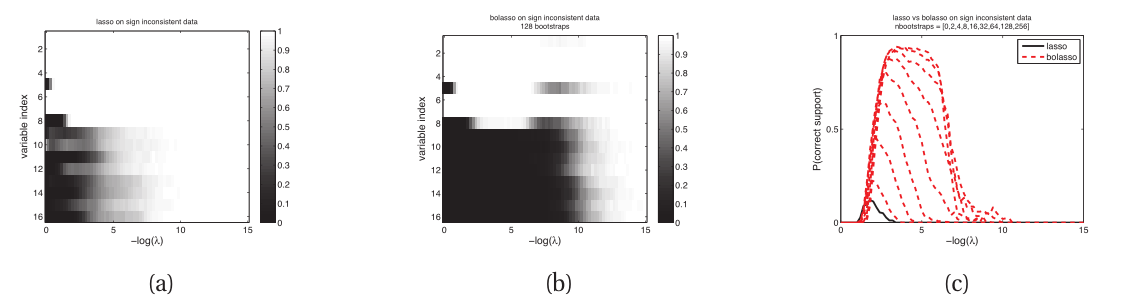
\includegraphics[width=0.7\linewidth]{fig13/figure10}
	\caption*{图13.10:(a)每个变量的选择概率(白色=大概率,黑色=小概率)与lasso正则化参数的关系。当我们从左向右移动时,我们减少正则化的量,因此选择更多的变量。(b) 与(a)相同,但适用于bolasso。(c) 符号正确估计的概率与正则化参数。Bolasso(红色,虚线)和Lasso(黑色,普通):引导复制的数量在\{2,4,8,16,32,64,128,256\}。基于(Bach 2008)的图1-3。图由bolassoDemo生成。}
\end{figure}

作为说明,我们复制了(Bach 2008)中的实验。特别是,我们创建了256个大小为N=1000的数据集,其中D=16个变量,其中8个是相关的。关于实验设置的更多细节,见(Bach 2008)。对于数据集n,变量j和稀疏程度k,定义$S(j,k,n)=\mathbb{I}(\hat{w}_j(\lambda_k,\mathcal{D}_n)\ne 0)$。现在定义$P(j,k)$为256个数据集上$S(j,k,n)$的平均值。在图13.10(a-b)中,我们绘制了lasso和bolasso的$P$与$-\log (\lambda)$的关系。我们看到,对于bolasso来说,有一个很大的$\lambda$范围,在这个范围内,真正的变量被选中,但对于lasso来说,情况并非如此。这一点在图13.10(c)中得到了强调,我们在图中绘制了拉索和博拉索的正确变量集被恢复的经验概率,随着引导样本数量的增加。当然,使用更多的样本需要更长的时间。在实践中,32个自举样本似乎是速度和准确性之间的一个很好的折中。

对于bolasso,通常存在选择$\lambda$的问题。显然,我们可以使用交叉验证,但图13.10(b)等图提出了另一种启发式方法:洗牌行以创建一个大的黑色块,然后选择$\lambda$位于该区域的中间。当然,操作这种直觉可能很棘手,需要各种特殊阈值(这让人想起第11.5.2节讨论如何为混合模型选择K时讨论的“在曲线中找到拐点”启发式)。贝叶斯方法为选择$\lambda$提供了更具原则性的方法。

\subsubsection{具有拉普拉斯先验的线性模型的贝叶斯推理}
我们一直专注于稀疏线性模型中的MAP估计。也可以进行贝叶斯推理(例如,参见(Park和Casella 2008;Seeger 2008))。然而,后验均值和中位数以及后验样本并不稀疏;只有模式是稀疏的。这是第5.2.1节中讨论的现象的另一个例子,在该节中,我们说MAP估计通常不典型于大部分后验值。

支持使用后验平均值的另一个论点来自等式5.108,该等式表明,如果我们想要最小化平方预测误差,插入后验平均值而不是后验模式是最佳做法。(Schniter等人,2008)在实验上表明,(Elad和Yavnch,2009)在理论上表明,使用具有尖峰和平板先验的后验平均值比使用具有拉普拉斯先验的后验模式具有更好的预测精度,尽管计算成本略高。

\subsection{$\ell_1$正则化:算法}
在本节中,我们简要回顾了一些可用于求解的算法$\ell_1$正则化估计问题。我们关注的是lasso情况,在这里我们有一个二次损失。然而,大多数算法可以扩展到更一般的设置,如逻辑回归(参见(Yaun等人,2010年),以全面审查$\ell_1$正则化逻辑回归)。请注意,机器学习的这一领域进展非常迅速,因此在阅读本章时,以下方法可能还不是最先进的。(见(Schmidt等人,2009;Yaun等人,2010;Yang等人2010)最近的一些调查。)

\subsubsection{坐标下降}
有时很难同时优化所有变量,但很容易逐个优化。特别是,我们可以在所有其他系数保持不变的情况下求解第j系数:
\begin{equation}
	w_j^*=\argmin_z\ f(\w+z\e_j)-f(\w)\tag{13.65}
\end{equation}
其中$\e_j$是第j个单位向量。我们可以以确定的方式在坐标中循环,也可以随机采样,或者可以选择更新梯度最陡的坐标。

如果每个一维优化问题都可以解析求解,则坐标下降法尤其有吸引力。例如,lasso的\textbf{射击算法}(Fu 1998;Wu和Lange 2008)使用等式13.54计算给定所有其他系数的$w_j$的最优值。伪代码见算法7(一些Matlab代码见LassoShooting)。

参见(Yaun等人,2010),了解该方法对逻辑回归案例的一些扩展。由此产生的算法是他们实验比较中最快的方法,它涉及到具有大量稀疏特征向量(代表一袋单词)的文档分类。其他类型的数据(例如密集特征和/或回归问题)可能需要不同的算法。


\renewcommand{\thealgorithm}{13.1}
\begin{algorithm}
	\caption{lasso坐标下降(又名射击算法)}
	\label{alg:A}
	\begin{algorithmic}[1]
		\STATE 初始化$\w=(\X^T\X+\lambda\I)^{-1}\X^T\y$
		\STATE 重复
		\STATE \ \ \ \ \ \textbf{for}\ $j=1$,...,$D$\ \textbf{do}
		\STATE \ \ \ \ \ \ \ \ \  $a_j=2\sum\nolimits_{i=1}^nx_{ij}^2$;
		\STATE \ \ \ \ \ \ \ \ \  $c_j=2\sum\nolimits_{i=1}^nx_{ij}(y_i-\w^T\x_i+w_jx_{ij})$;
		\STATE \ \ \ \ \ \ \ \ \ $w_j$=soft($\frac{c_j}{a_j}$,$\frac{\lambda}{a_j}$);
		\STATE 直到收敛
	\end{algorithmic}
\end{algorithm}
\subsubsection{LARS和其他同构方法}
坐标下降的问题是,它一次只更新一个变量,因此收敛速度较慢。\textbf{活动集}方法一次更新许多变量。不幸的是,它们更复杂,因为需要识别哪些变量被约束为零,哪些变量可以自由更新。

活动集方法通常一次只添加或删除几个变量,因此如果开始时远离解决方案,则可能需要很长时间。但它们非常适合从空集开始,为$\lambda$的不同值生成一组解,即生成正则化路径。这些算法利用了一个事实,即可以从$\hat{\w}(\lambda_k)$快速计算$\hat{\w}(\lambda_{k-1})$如果$\lambda_k\approx \lambda_{k-1}$.这被称为\textbf{温启动}。事实上,即使我们只需要$\lambda$的单个值的解,也可以称之为$\lambda_*$, 有时计算一组解(从$\lambda_{max}$到$\lambda_*$)在计算上更有效, 使用温启动;这被称为延拓方法或同伦方法。这通常比在$\lambda_*$处直接“冷启动”快得多; 尤其如果$\lambda_*$是小的。

机器学习中同构方法最著名的例子可能是\textbf{LARS}算法,它代表“最小角度回归和收缩”(Efron等人,2004)(在(Osborne等人,2000b,a)中独立发明了一种类似的算法)。这可以有效地计算$\lambda$的所有可能值的$\hat{\w}(\lambda)$.

LARS的工作如下。它从较大的$\lambda$值开始,因此仅选择与响应向量$\y$最相关的变量。然后减小$\lambda$,直到找到第二个变量,该变量与第一个变量的电流残差具有相同的相关性(在幅值方面),其中步骤k处的残差定义为$\r_k=\y-\X_{:,F_k}\w_k$,其中$F_k$是当前\textbf{活动集}(c.f.,等式13.50)。值得注意的是,可以通过使用几何参数(因此称为“最小角度”)解析求解$\lambda$的这个新值。这使得算法能够快速“跳转”到正则化路径上的下一个点,在该点上活动集发生变化。重复该操作,直到添加所有变量。

如果我们希望解序列对应于lasso的正则化路径,则有必要允许从活动集移除变量。如果我们不允许删除变量,我们会得到一个稍微不同的算法,称为\textbf{LAR},它往往更快。特别是,LAR的成本与单个普通最小二乘拟合相同,即$O(NDmin(N,D)),$,如果$N>D$,则为$O(ND^2)$,如果$D>N$,则为$O(N^2D)$。LAR非常类似于贪婪正向选择,以及一种称为最小二乘增强的方法(见第16.4.6节)。

有许多人试图扩展LARS算法来计算全正则化路径$\ell_1$正则化GLMs,如逻辑回归。通常,无法解析求解$\lambda$的临界值。相反,标准方法是从$\lambda_{max}$开始,然后缓慢减小$\lambda$,在我们前进的过程中跟踪解决方案;这被称为\textbf{延拓方法或同构方法}。这些方法利用了这样一个事实,即我们可以从$\hat{\w}(\lambda_{k})$快速计算$\hat{\w}(\lambda_{k-1})$如果$\lambda_{k}\approx \lambda_{k-1}$.这被称为\textbf{温启动}。即使我们不想要完整的路径,这种方法通常比在所需的$\lambda$值下直接“冷启动”快得多(如果$\lambda$很小,尤其如此)。

(Friedman等人,2010)中描述的方法将坐标下降与该预热启动策略相结合,并计算任何$\ell_1$正则GLM。这已在glmnet包中实现,该包与PMTK捆绑在一起。

\subsubsection{近端和梯度投影方法}
在本节中,我们考虑了一些适用于超大规模问题的方法,其中同伦方法的速度太慢。除了$\ell_1$,我们稍后将看到。我们在本节中的介绍基于(Vandenberghe 2011;Yang等人,2010)。

考虑形式的凸目标
\begin{equation}
	f(\boldsymbol{\theta})=L(\boldsymbol{\theta})+R(\boldsymbol{\theta})\tag{13.66}
\end{equation}
其中,$L(\boldsymbol{\theta})$(表示损失)是凸的且可微的,而$R(\boldsymbol{\theta})$(表示正则化子)是凸但不一定可微的。例如,$L(\boldsymbol{\theta})=RSS(\boldsymbol{\theta})$和$R(\boldsymbol{\theta})=\lambda||\boldsymbol{\theta}||_1$; 对应于BPDN问题。作为另一个例子,lasso问题可以表示为:$L(\boldsymbol{\theta})=RSS(\boldsymbol{\theta})$和$R(\boldsymbol{\theta})=\I_C(\boldsymbol{\theta})$,其中$C=\{\boldsymbol{\theta}:||\boldsymbol{\theta}||_1\le B\}$,$\I_C(\boldsymbol{\theta})$是凸集C的指示函数,定义为

\begin{equation}
	I_C(\boldsymbol{\theta})\triangleq \left\{
	\begin{array}{ll}
	0 &  \boldsymbol{\theta}\in C\\
	+\infty & otherwise 
	\end{array} \right.\tag{13.67}
\end{equation}

在某些情况下,很容易优化方程13.66中形式的函数。例如,假设$L(\boldsymbol{\theta})=RSS(\boldsymbol{\theta})$,设计矩阵简单地为$\X=\I$。然后目标变为$f(\boldsymbol{\theta})=R(\boldsymbol{\theta})+\frac{1}{2}||\boldsymbol{\theta}-\y||_2^2$。其最小值由$prox_R(\y)$出,它是凸函数R的\textbf{近似算子},定义如下:
\begin{equation}
	prox_R(\y)=\argmin_\z(R(\z)+\frac{1}{2}||\z-\y||_2^2)\tag{13.68}
\end{equation}

直观地说,我们返回的是一个使R最小化但也接近(接近)$\y$的点。一般来说,我们将在迭代优化器中使用该操作符,在这种情况下,我们希望与前一个迭代保持接近。在这种情况下,我们使用

\begin{equation}
prox_R(\boldsymbol{\theta}_k)=\argmin_\z(R(\z)+\frac{1}{2}||\z-\boldsymbol{\theta}_k||_2^2)\tag{13.69}
\end{equation}

关键问题是:如何有效地计算不同正则化子R的近似算子,以及如何将该技术扩展到更一般的损失函数L?我们将在下面讨论这些问题。
\subsubsection*{13.4.3.1 近端操作器}
如果$R(\boldsymbol{\theta})=\lambda||\boldsymbol{\theta}||_1$,则通过分量软阈值给出近端算子:

\begin{equation}
	prox_R(\boldsymbol{\theta})=soft(\boldsymbol{\theta},\lambda)\tag{13.70}
\end{equation}
如我们在第13.3.2节中所示,如果$R(\boldsymbol{\theta})=\lambda||\boldsymbol{\theta}||_0$;则通过分量硬阈值给出近似算子:
\begin{equation}
	prox_R(\boldsymbol{\theta})=hard(\boldsymbol{\theta},\sqrt{2\lambda})\tag{13.71}
\end{equation}

其中$hard(u,a)\triangleq u\mathbb{I}(|u|>a)$

如果$R(\boldsymbol{\theta})=\I_C(\boldsymbol{\theta})$,则通过投影到集合C上给出近端算子:
\begin{equation}
	prox_R(\boldsymbol{\theta})=\argmin_{\z\in C}||\z-\boldsymbol{\theta}||_2^2=proj_C(\boldsymbol{\theta})\tag{13.72}
\end{equation}

\begin{figure}[h]
	\centering
	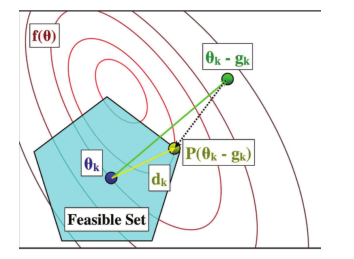
\includegraphics[width=0.7\linewidth]{fig13/figure11}
	\caption*{图13.11:投影梯度下降示意图。沿负梯度的步长,到$\boldsymbol{\theta}_k-\g_k$将我们带到可行集之外。如果我们将该点投影到集合中最近的点上,我们得到$\boldsymbol{\theta}_{k+1}=proj_{\varTheta}(\boldsymbol{\theta}_k-\g_k)$。然后,我们可以使用$\d_k=\boldsymbol{\theta}_{k+1}-\boldsymbol{\theta}_{k}$推导隐式更新方向。经马克·施密特许可使用。}
\end{figure}

对于某些凸集,很容易计算投影算子。例如,投影到长方体约束定义的矩形集$C=\{\boldsymbol{\theta}:\ell_j\le \theta_j\le u_j\}$我们可以使用

\begin{equation}
	proj_C(\boldsymbol{\theta})_j=\left\{
	\begin{array}{cl}
	\ell_j& \theta_j\le \ell_j\\
	\theta_j& \ell_j\le \theta_j\le u_j\\
	u_j& \theta_j\ge u_j
	\end{array}\right. \tag{13.73}
\end{equation}

投影到欧几里得球$C=\{\boldsymbol{\theta}:||\boldsymbol{\theta}||_2\le 1\}$我们可以使用

\begin{equation}
	proj_C(\boldsymbol{\theta})=\left\{
	\begin{array}{cl}
	\frac{\boldsymbol{\theta}}{||\boldsymbol{\theta}||_2}& ||\boldsymbol{\theta}||_2>1 \\
	\boldsymbol{\theta}& ||\boldsymbol{\theta}||_2\le 1
	\end{array}\right. \tag{13.74}
\end{equation}

投影到1-范数球$C=\{\boldsymbol{\theta}:||\boldsymbol{\theta}||_1\le 1\}$我们可以使用

\begin{equation}
	proj_C(\boldsymbol{\theta})=soft(\boldsymbol{\theta},\lambda)\tag{13.75}
\end{equation}

其中$\lambda=0$,如果$||\boldsymbol{\theta}||_1\le 1$,否则$\lambda$是方程的解
\begin{equation}
	\sum_{j=1}^{D}max(|\theta_j|-\lambda,0)=1\tag{13.76}
\end{equation}

如(Duchi等人,2008)所述,我们可以在$O(D)$时间内实现整个过程。

我们将在第13.5.1.2节中看到这些不同投影方法的应用。

\subsubsection*{13.4.3.2  近端梯度法}

我们现在讨论如何在梯度下降例程中使用近似算子。基本思想是最小化损失函数的简单二次近似,$\boldsymbol{\theta}_k$ 为中心

\begin{equation}
\boldsymbol{\theta}_{k+1}=\argmin_\z  R(\z)+L(\boldsymbol{\theta}_k)+\g_k^T(\z -\boldsymbol{\theta}_k)+\frac{1}{2t_k}||\z -\boldsymbol{\theta}_k||_2^2\tag{13.77}
\end{equation}
其中$\g_k=\nabla L(\boldsymbol{\theta_k})$是损耗的梯度,$t_k$是下面讨论的常数,最后一项来自于对形式损耗的海森近似$\nabla^2L(\boldsymbol{\theta}_k)\approx \frac{1}{t_k}\I$.

去掉与$\z$无关的项,然后乘以$t_k$,我们可以根据近似算子重写上述表达式,如下所示:
\begin{align}
\boldsymbol{\theta}_{k+1}\ &=\ \argmin_\z \left[t_k R(\z)+\frac{1}{2}||\z-\u_k||_2^2\right]=prox_{t_kR}(\u_k)\tag{13.78}\\
\u_k\ &=\ \boldsymbol{\theta}_{k}-t_k\g_k\tag{13.79}\\
\g_k\ &=\ \nabla L(\boldsymbol{\theta}_k)\tag{13.80}
\end{align}
如果$R(\boldsymbol{\theta})=0$,这相当于\textbf{梯度下降}。如果$R(\boldsymbol{\theta})=\I_C(\boldsymbol{\theta})$,则该方法等效于投影梯度下降,如图13.11所示。如果$R(\boldsymbol{\theta})=\lambda||\boldsymbol{\theta}||_1$,则该方法称为\textbf{迭代软阈值}。

有几种方法可以选择$t_k$,或者等效地,$\alpha_k=1/t_k$。假设$\alpha_k \I$是Hessian方程的近似值$\nabla^2L$,我们需要
\begin{equation}
	\alpha_k(\boldsymbol{\theta}_k-\boldsymbol{\theta}_{k-1})\approx \g_k-\g_{k-1}\tag{13.81}
\end{equation}
在最小二乘意义上。因此
\begin{equation}
	\alpha_k=\argmin_\alpha||\alpha(\boldsymbol{\theta}_k-\boldsymbol{\theta}_{k-1})-(\g_k-\g_{k-1})||_2^2=\dfrac{(\boldsymbol{\theta}_k-\boldsymbol{\theta}_{k-1})^T(\g_k-\g_{k-1})}{(\boldsymbol{\theta}_k-\boldsymbol{\theta}_{k-1})^T(\boldsymbol{\theta}_k-\boldsymbol{\theta}_{k-1})}\tag{13.82}
\end{equation}
这被称为\textbf{Barzilai-Borwein}(BB)或\textbf{光谱步长}(Barzilay和Borwein1988;Fletcher 2005;Raydan 1997)。该步长可用于任何梯度方法,无论是否接近。它不会导致目标的单调减少,但比标准的线搜索技术快得多。(为了确保收敛,我们要求目标“平均”减少,其中平均值是在大小为M+1的滑动窗口上计算的。)

当我们将BB步长与迭代软阈值技术(对于$R(\boldsymbol{\theta})=\lambda||\boldsymbol{\theta}||_1$结合起来,再加上逐渐减小$\lambda$的连续方法时,我们得到了一种用于BPDN问题的快速方法,称为SpaRSA算法,它代表“通过可分离近似进行稀疏重建”(Wright等人,2009)。然而,我们将其称为迭代收缩和阈值算法。一些伪代码见算法12,一些Matlab代码见SpaRSA。另请参见练习13.11,了解基于投影梯度下降的相关方法。

\subsubsection*{13.4.3.3 Nesterov方法}
通过围绕非最新参数值的点进行二次近似,可以获得更快的近似梯度下降。特别是,考虑更新表单
\begin{align}
	\boldsymbol{\theta}_{k+1}\ &=\ prox_{t_kR}(\phi
_k-t_k\g_k)\tag{13.83}\\
\g_k\ &=\ \nabla L(\phi_k)\tag{13.84}\\
\phi_k\ &=\ \boldsymbol{\theta}_k+\dfrac{k-1}{k+2}(\boldsymbol{\theta}_k-\boldsymbol{\theta}_{k-1})\tag{13.85}
\end{align}


\renewcommand{\thealgorithm}{13.2}
\begin{algorithm}
	\caption{迭代收缩阈值算法(ISTA)}
	\label{alg:A}
	\begin{algorithmic}[1]
		\STATE 输入:$\X \in \mathbb{R}^{N\times D},\y \in \mathbb{R}^N $参数$\lambda\ge 0,M\ge 1,0<s<1$
		\STATE 初始化 $\boldsymbol{\theta}_0=\0,\alpha=1,\r=\y ,\lambda_0=\infty$
		\STATE 重复
		\STATE \ \ \ \ \ $\lambda_t=max(s||\X^T\r||_\infty,\lambda)$ //调整正则化器
		\STATE \ \ \ \ \ 重复
		\STATE \ \ \ \ \ \ \ \ \  $\g =\nabla L(\boldsymbol{\theta})$;
		\STATE \ \ \ \ \ \ \ \ \  $\u =\boldsymbol{\theta}-\frac{1}{\alpha}\g$ ;
		\STATE \ \ \ \ \ \ \ \ \  $\boldsymbol{\theta}=soft(\u ,\frac{\lambda_t}{\alpha})$
		\STATE \ \ \ \ \ \ \ \ \  使用等式13.82中的BB步长更新$\alpha$;
		\STATE \ \ \ \ \ 直到$f(\boldsymbol{\theta})$在过去的M步内增加过多
		\STATE \ \ \ \ \ $\r=\y \X\boldsymbol{\theta}$//更新残差
		\STATE 直到$\lambda_t=\lambda$
	\end{algorithmic}
\end{algorithm}

\begin{figure}[h]
	\centering
	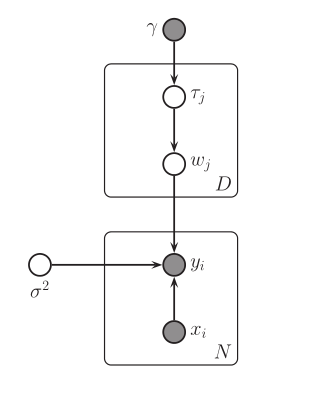
\includegraphics[width=0.5\linewidth]{fig13/figure12}
	\caption*{图13.12: 使用高斯尺度混合表示lasso。}
\end{figure}
这就是\textbf{Nesterov的方法}(Nesterov 2004;Tseng 2008)。和以前一样,有多种设置$t_k$的方法;通常使用线搜索。

当该方法与迭代软阈值技术(对于$R(\boldsymbol{\theta})=\lambda||\boldsymbol{\theta}||_1$结合,再加上逐渐减小$\lambda$的连续方法时,我们得到了一种求解BPDN问题的快速方法,称为\textbf{快速迭代收缩保持算法或FISTA}(Beck和T eboulle 2009)。

\subsubsection{EM代表lasso}
在本节中,我们将展示如何使用lasso解决lasso问题。乍一看,这似乎有些奇怪,因为没有隐藏的变量。关键的见解是,我们可以将拉普拉斯分布表示为\textbf{高斯尺度混合}(GSM)(Andrews and Mallows 1974;West 1987),如下所示:
\begin{equation}
	Lap(w_j|0,1/\gamma)=\frac{\gamma}{2}e^{-\gamma|w_j|}=\int \mathcal{N}(w_j|0,\tau_j^2)Ga(\tau_j^2|1,\frac{\gamma^2}{2})d\tau_j^2\tag{13.86}
\end{equation}
因此,拉普拉斯是一个GSM,其中方差上的混合分布是指数分布,Expon$(\tau_j^2|\frac{\gamma^2}{2}=Ga(\tau_j^2|1,\frac{\gamma^2}{2}))$。使用这种分解,我们可以表示如图13.12所示的套索模型。相应的联合分布具有以下形式
\begin{align}
	p(\y,\w,\boldsymbol{\tau},\sigma^2|\X )\ \ =\ &\mathcal{N}(\y|\X\w,\sigma^2\I_N)\mathcal{N}(\w|\0,\D_r)\tag*{}\\
	&\I\G(\sigma^2|a_\sigma,b_\sigma)\left[\prod_j Ga(\tau_j^2|1,\gamma^2/2) \right]\tag{13.87}
\end{align}
其中$\D_\tau =diag(\tau_j^2)$,并且为了简化符号,我们假设$\X$是标准化的,$\y$是中心的(因此我们可以忽略偏移项$\mu$)。通过扩展,我们得到了

\begin{align}
	p(\y,\w,\boldsymbol{\tau},\sigma^2|\X )\varpropto &(\sigma^2)^{-N/2}exp\left(-\frac{1}{2\sigma^2}||\y-\X\w||_2^2\right)|\D_\tau |^{-\frac{1}{2}}\tag*{}\\
	&exp\left(-\frac{1}{2}\w^T\D_\tau \w\right)(\sigma^2)^{-(a_\sigma+1)}\tag*{}\\
	&exp(-b_\sigma/\sigma^2)\prod_jexp(-\frac{\gamma^2}{2}\tau_j^2)\tag{13.88}
\end{align}

下面,我们简要描述了如何将EM算法应用于图13.12.\footnote{为了确保后验是单峰的,可以遵循(Park和Casella,2008),并通过使权重的先验方差取决于观测噪声来略微修改模型:$p(w_j|\tau_j^2,\sigma^2)=\mathcal{N}(w_j|0,\sigma^2\tau_j^2)$。EM算法易于修改。}中的模型。在E步骤中,我们推断$\tau_j^2$和$\sigma^2$,在M步骤中我们估计$\w$。所得估计$\hat{\w}$与lasso估计相同。这种方法最早是在(Figueiredo,2003年)提出的(一些扩展请参见(Griffin和Brown,2007年;Caron和Doucet,2008年;Ding和Harrison,2010年)。

\subsubsection*{13.4.4.1  为什么是EM?}
在深入研究EM的细节之前,值得一问的是,既然有多种其他(通常更快)算法可以直接解决问题,我们为什么要提出这种方法$\ell_1$MAP估计问题(经验比较见Linregfitl1检验)。原因是潜在变量视角带来了几个优势,例如:
\begin{itemize}
\item  它提供了一种简单的方法来推导一个算法来查找各种其他模型的$\ell_1-$正则化参数估计,如稳健线性回归(练习11.12)或概率回归(练习13.9)。
\item 它建议尝试除$Ga(\tau_j^2|1,\gamma^2/2)$之外的其他方差先验。我们将在下面考虑各种扩展。
\item 它清楚地说明了我们如何计算全后验概率$p(\w|D)$,而不仅仅是一个MAP估计。这种技术被称为\textbf{贝叶斯lasso}(Park和Casella 2008;Hans 2009)。
\end{itemize}

\subsubsection*{13.4.4.2  目标函数}
从等式13.88中,完整数据惩罚对数似然如下(不依赖于$\w$的下降项)
\begin{equation}
	\ell_c(\w)=-\frac{1}{2\sigma^2}||\y-\X\w||_2^2-\frac{1}{2}\w^T\Lambda\w+const\tag{13.89}
\end{equation}
其中$\Lambda=diag(\frac{1}{\tau_j^2})$是$\w$的精度矩阵。

\subsubsection*{13.4.4.3 E步骤}
关键是计算$\mathbb{E}\left[\frac{1}{\tau_j^2}|w_j\right]$,我们可以直接推导出(见练习13.8)。或者,我们可以推导出完整的后验概率,如下所示(Park和Casella,2008):
\begin{equation}
	p(1/\tau_j^2|\w,D)=InverseGaussian\left(\sqrt{\frac{\gamma^2}{w_j^2}},\gamma^2\right)\tag{13.90}
\end{equation}
(注意,\textbf{逆高斯分布}也称为Wald分布。)因此
\begin{equation}
	\mathbb{E}\left[\frac{1}{\tau_j^2}|w_j\right]=\frac{\gamma}{|w_j|}\tag{13.91}
\end{equation}
设$\overline{\Lambda}=diag(\mathbb{E}[1/\tau_1^2],...,\mathbb{E}[1/\tau_D^2])$表示该E步的结果.

我们还需要推断$\sigma^2$。很容易证明后验概率是
\begin{equation}
	p(\sigma^2|D,\w)=IG(a_\sigma+(N)/2,b_\sigma+\frac{1}{2}(\y-\X\hat{\w})^T(\y-\X\hat{\w}))=IG(a_N,b_N)\tag{13.92}
\end{equation}
因此
\begin{equation}
	\mathbb{E}[1/\sigma^2]=\frac{a_N}{b_N}\triangleq \overline{\omega}\tag{13.93}
\end{equation}

\subsubsection*{13.4.4.4  M步骤}
M步骤包括计算
\begin{equation}
	\hat{\w}=\argmax_\w-\frac{1}{2}\overline{\omega}||\y-\X\w||_2^2-\frac{1}{2}\w^T\Lambda\w\tag{13.94}
\end{equation}
这只是高斯先验下的MAP估计:
\begin{equation}
	\hat{\w}=(\sigma^2\overline{\Lambda}+\X^T\X)^{-1}\X^T\y\tag{13.95}
\end{equation}
然而,由于我们预期许多$w_j=0$,因此对于许多j,我们将得到$\tau_j^2=0$。这使得反演$\overline{\Lambda}$在数值上不稳定。幸运的是,我们可以使用$\X$的奇异值分解,由$\X=\U\D\V^T$给出,如下所示:
\begin{equation}
	\hat{\w}=\Psi\V(\V^T\Psi\V+\frac{1}{\overline{\omega}}\D^{-2})^{-1}\D^{-1}\U^T\y\tag{13.96}
\end{equation}
其中
\begin{equation}
	\Psi=\overline{\Lambda}^{-1}=diag(\dfrac{1}{\mathbb{E}[1/\tau_j^2]})=diag[\dfrac{|w_j|}{\pi'(w_j)}]\tag{13.97}
\end{equation}

\subsubsection*{13.4.4.5  警告}
由于lasso目标是凸的,该方法应始终找到全局最优值。不幸的是,由于数字原因,这种情况有时不会发生。特别地,假设在真解中$w_j^*\ne 0$,进一步,假设我们在M步中设置$\hat{\w}_j=0$。在接下来的E步中,我们推断$\tau_j^2=0$,因此我们再次设置$\hat{\w}_j=0$;因此,我们永远无法“撤消”我们的错误。幸运的是,在实践中,这种情况似乎很少见。进一步讨论请参见(Hunter和Li,2005)。

\subsection{$\ell_1$正则化:扩展}
在本节中,我们将讨论“vanilla”的各种扩展$\ell_1$正则化。
\subsubsection{lasso组}
在标准中$\ell_1$正则化,我们假设参数和变量之间存在1:1的对应关系,因此如果$\hat{w}_j=0$,我们将其解释为变量j被排除在外。但在更复杂的模型中,可能有许多参数与给定变量相关。特别是,我们可能有每个输入的权重向量$\w_j$。以下是一些例子:
\begin{itemize}
\item \textbf{多项式逻辑回归}:每个特征与C个不同的权重相关,每个类别一个。
\item \textbf{带分类输入的线性回归}:每个标量输入是一个热编码到长度为C的向量中。
\item \textbf{多任务学习}在多任务学习中,我们有多个相关的预测问题。例如,我们可能有C独立回归或二元分类问题。因此,每个特征与C个不同的权重相关联。我们可能希望对所有任务使用一个功能,或者不使用任何任务,从而在组级别选择权重(Obozinski等人。2007).
\end{itemize}

如果我们使用形式为$||\w||=\sum\nolimits_{j}\sum\nolimits_{c}|w_{jc}|$的$\ell_1$正则化子,我们可能最终得到$\w_{j,:}$的某些元素为零,而有些元素不为零。为了防止这种情况,我们将参数向量划分为G组。我们现在最小化以下目标:
\begin{equation}
	J(\w)=NLL(\w)+\sum_{g=1}^{G}\lambda_g||\w_g||_2\tag{13.98}
\end{equation}
其中
\begin{equation}
	||\w_g||_2=\sqrt{\sum_{j\in g}w_j^2}\tag{13.99}
\end{equation}
是组权重向量的2-范数。如果NLL是最小二乘法,这种方法称为\textbf{lasso组}(Yuan和Lin,2006)。

我们通常通过设置$\lambda_g=\lambda\sqrt{d_g}$,其中$d_g$是群g中元素的数目。例如,如果我们有群$\{1,2\}$和$\{3,4,5\}$,目标就变成了
\begin{equation}
	J(\w)=NLL(\w)+\lambda\left[\sqrt{2}\sqrt{(w_1^2+w_2^2)}+\sqrt{3}\sqrt{(w_3^2+w_4^2+w_5^2)}\right]\tag{13.100}
\end{equation}
请注意,如果我们使用了2-范数的平方,该模型将等价于岭回归,因为
\begin{equation}
	\sum_{g=1}^{G}||\w_g||_2^2=\sum_{g}\sum_{j\in g}w_j^2=||\w||_2^2\tag{13.101}
\end{equation}
通过使用平方根,我们惩罚了包含群权重向量的球的半径:半径变小的唯一方法是所有元素都变小。因此,平方根导致群稀疏。

该技术的一种变体将2-范数替换为无穷范数(Turlach等人2005;Zhao等人2005):
\begin{equation}
	||\w_g||_\infty =\max_{j\in g}|w_j|\tag{13.102}
\end{equation}
很明显,这也会导致群体稀疏。

图13.13和13.14显示了差异的说明。在这两种情况下,我们都有一个大小为$D=2^{12}=4096$的真实信号$\w$,分为64组,每组大小为64。我们随机选择8组$\w$,并将其分配为非零值。在第一个示例中,这些值是从$\mathcal{N}(0,1)$中提取的。在第二个示例中,所有值都设置为1。然后,我们选择一个大小为$N\times D$的随机设计矩阵$\X$,其中$N=2^{10}=1024$。最后,我们生成$\y=\X\w+\epsilon$,其中$\epsilon \sim\mathcal{N}(\0,10^{-4}\I_N)$。鉴于这些数据,我们使用$\ell_1$或组$\ell_1$然后使用最小二乘法估计非零值。我们看到群套索比香草套索做得更好,因为它尊重已知的群结构。\footnote{系统中轻微的非零“噪音”$\ell_\infty$组lasso结果可能是由于数值误差。}我们也看到了$\ell_\infty$范数倾向于使块内的所有元素具有相似的大小。这适用于第二个示例,但不适用于第一个示例。($\lambda$的值在所有示例中都相同,并且是手动选择的。)

\subsubsection*{13.5.1.1 群lasso的GSM解释}
组lasso等价于使用以下先验知识的MAP估计:
\begin{equation}
p(\w|\gamma,\sigma^2) \propto exp\left(-\frac{\gamma}{\sigma}\sum_{g=1}^{G}||\w_g||_2\right)\tag{13.103}
\end{equation}

\begin{figure}[h]
	\centering
	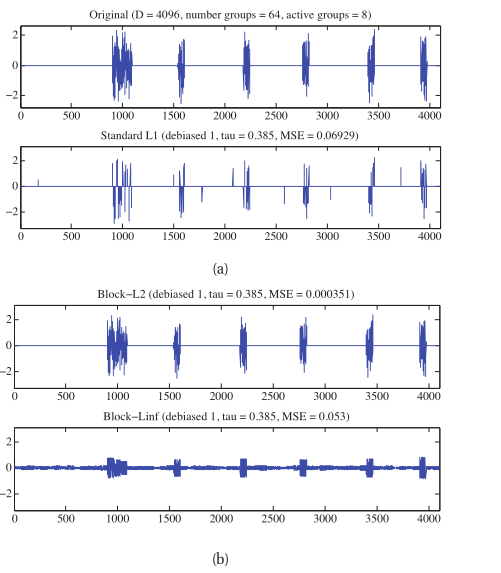
\includegraphics[width=0.5\linewidth]{fig13/figure13}
	\caption*{图13.13:原始信号为分段高斯的群套索示意图。左上角:原始信号。左下:vanilla lasso估计。左上:使用组lasso估计块上的$\ell_2$范数。右下角:使用$\ell_\infty$范数。根据(Wright等人。2009).图由groupLassoDemo根据Mario Figueiredo的代码生成。}
\end{figure}
现在可以证明(练习13.10),该先验可以写成GSM,如下所示:
\begin{align}
	\w_g|\sigma^2,\tau_g^2\ \ &\sim \ \ \mathcal{N}(\0,\sigma^2\tau_g^2\I_{d_g})\tag{13.104}\\
	\tau_g^2|\gamma\ \ &\sim\ \ Ga(\dfrac{d_g+1}{2},\frac{\gamma}{2})\tag{13.105}
\end{align}
其中$d_g$是群g的大小。因此我们看到每组有一个方差项,每个方差项来自伽马先验,其形状参数取决于群大小,其速率参数由$\gamma$控制。图13.15给出了一个示例,其中我们有两个组,一个大小为2,一个为3。

这幅图也清楚地说明了为什么应该有分组效应。假设$w_{1,1}$,1很小;则$\tau_1^2$将被估计为小,这将迫使$w_{1,2}$变小。反之,假设$w_{1,1}$较大;则$\tau_1^2$将被估计为大,这将允许$w_{1,2}$也变大。

\begin{figure}[h]
	\centering
	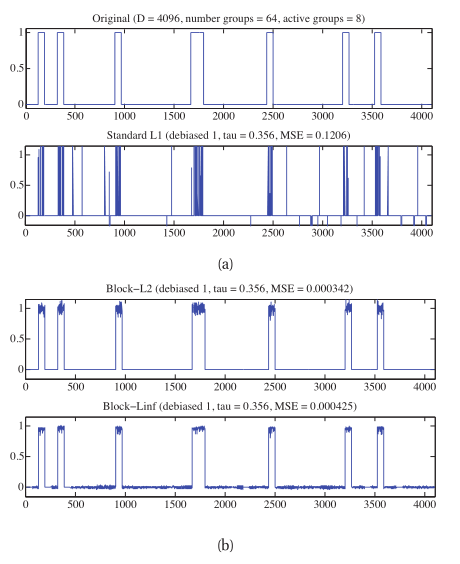
\includegraphics[width=0.4\linewidth]{fig13/figure14}
	\caption*{图13.14与图13.13相同,只是原始信号是分段恒定的。}
\end{figure}


\begin{figure}[h]
	\centering
	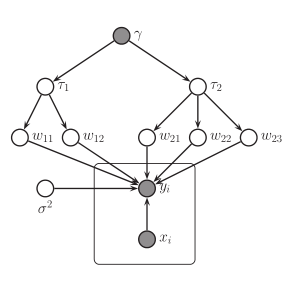
\includegraphics[width=0.4\linewidth]{fig13/figure15}
	\caption*{图13.15两组lasso的图形模型,第一组的尺寸$G_1$=2,第二组的尺寸$G_2$=3。}
\end{figure}

\subsubsection*{13.5.1.2 群lasso算法}
群lasso有多种算法。这里我们简要地提到两个。第一种方法基于第13.4.3节中讨论的近端梯度下降。由于正则化子是可分离的,$R(\w)=\sum\nolimits_{g}||\w_g||_p$,近端算子分解为G个形式的独立算子

\begin{equation}
	prox_R(\b)\argmin_{\z\in \mathbb{R}^{D_g}}||\z-\b||_2^2+\lambda||\z||_p\tag{13.106}
\end{equation}
其中$\b=\boldsymbol{\theta}_{kg}-t_k\g_{kg}$。如果p=2,可以证明(Combettes和Wajs 2005),这可以实现如下
\begin{equation}
prox_R(\b)=\b -proj_{\lambda C}(\b)\tag{13.107}
\end{equation}
其中$C=\{\z:||\z||_2\le 1\}$ 是$\ell_2$球。使用等式13.74,如果
$||\b||_2<\lambda$,则我们得到
\begin{equation}
	prox_R(\b)=\b-\b=\0\tag{13.108}
\end{equation}

否则,我们有
\begin{equation}
	prox_R(\b)=\b-\lambda\frac{\b}{||\b||_2}=\b\frac{||\b||_2-\lambda}{||\b||_2}\tag{13.109}
\end{equation}

我们可以将这些组合成向量软阈值函数,如下所示(Wright等人,2009):
\begin{equation}
	prox_R(\b)=\b\dfrac{max(||\b||_2-\lambda,0)}{max(||\b||_2-\lambda,0)+\lambda}\tag{13.110}
\end{equation}

如果$p=\infty$, 我们使用$C=\{\z:||\z||_1\le 1\}$ 是$\ell_1$球。我们可以使用(Duchi et al.2008)中描述的算法在$O(d_g)$时间内对此进行投影。

另一种方法是修改EM算法。该方法几乎与vanilla lasso相同。如果我们定义$\tau_j^2=\tau_{g(j)}^2$,则$g(j)$是维数j所属的群,我们可以像以前一样对$\sigma^2$和$\w$使用相同的全条件。唯一的变化如下:

\begin{itemize}
\item 我们必须修改权重精度的完整条件,该条件基于一组共享权重进行估计:
\begin{equation}
\frac{1}{\tau_g^2}|\gamma,\w,\sigma^2,\y,\X\sim InverseGaussian(\sqrt{\frac{\gamma^2\sigma^2}{||\w_g||_2^2}},\gamma^2)\tag{13.111}
\end{equation}

其中$||\w_g||_2^2=\sum\nolimits_{j\in g}w_{jg}^2$。对于E步骤,我们可以使用
\begin{equation}
	\mathbb{E}\left[\frac{1}{\tau_g^2}\right]=\frac{\gamma^\sigma}{||\w_g||_2}\tag{13.112}
\end{equation}
\item 我们必须修改调谐参数的完整条件,现在仅根据$\tau_g^2$的G值进行估计:
\begin{equation}
	p(\gamma^2|\tau)=Ga(a_\gamma+G/2,b_\gamma+\frac{1}{2}\sum_{g}^{G}\tau_g^2)\tag{13.113}
\end{equation}
\end{itemize}

\begin{figure}[h]
	\centering
	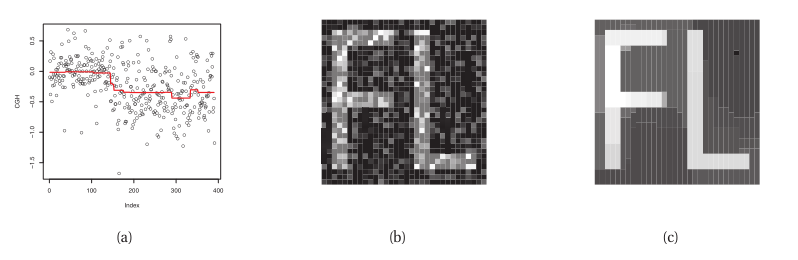
\includegraphics[width=0.7\linewidth]{fig13/figure16}
	\caption*{图13.16:(a)融合lasso的示例。纵轴表示阵列CGH(染色体基因组杂交)强度,横轴表示沿基因组的位置。资料来源:图1(Hoefling 2010)。(b) 噪声图像。(c) 使用2d晶格先验的融合lasso估计。资料来源:图2(Hoefling 2010)。经霍尔格·霍夫林许可使用。}
\end{figure}

\subsubsection{融合lasso}
在某些问题设置中(例如,函数数据分析),除了稀疏之外,我们还希望相邻系数彼此相似。图13.16(a)中给出了一个示例,其中我们希望拟合一个主要为“关闭”的信号,但另外还有一个特性,即相邻位置的值通常相似。我们可以使用该形式的先验知识对此进行建模

\begin{equation}
	p(\w|\sigma^2)\propto exp\left(-\frac{\lambda_1}{\sigma}\sum_{j=1}^{D}|w_j|-\frac{\lambda_2}{\sigma}\sum_{j=1}^{D-1}|w_{j+1}-w_j|\right)\tag{13.114}
\end{equation}
这就是所谓的\textbf{融合lasso}惩罚。在功能数据分析中,我们通常使用$\X=\I$,因此信号中的每个位置都有一个系数(见第4.4.2.3节)。在这种情况下,总体目标具有以下形式:
\begin{equation}
	J(\w,\lambda_1,\lambda_2)=\sum_{i=1}^{N}(y_i-w_i)^2+\lambda_1\sum_{i=1}^{N}|w_i|+\lambda_2\sum_{i=1}^{N-1}|w_{i+1}-w_i|\tag{13.115}
\end{equation}
这是等式4.148的稀疏版本。

可以将这一思想推广到链之外,并考虑其他图结构,使用形式惩罚
\begin{equation}
	J(\w,\lambda_1,\lambda_2)=\sum_{s\in V}(y_s-w_s)^2+\lambda_1\sum_{s\in V}|w_s|+\lambda_2\sum_{(s,t)\in E}|w_{s}-w_t|\tag{13.116}
\end{equation}
这被称为\textbf{图引导融合lasso}(参见例如(Chen等人2010))。该图可能来自一些先验知识,例如来自已知生物途径的数据库。另一个示例如图13.16(b-c)所示,其中图形结构为二维晶格。

\subsubsection*{13.5.2.1 融合lasso的GSM解释}
可以证明(Kyung等人,2010年),融合lasso模型等同于以下分层模型:
\begin{align}
	\w|\sigma^2,\boldsymbol{\tau},\boldsymbol{\omega} \ &\sim\ \mathcal{N}(\0,\sigma^2\textstyle\sum(\boldsymbol{\tau},\boldsymbol{\omega}))\tag{13.117}\\
	\tau_j^2|\gamma_1\ &\sim\ Expon(\frac{\gamma_1^2}{2}),j=1:D\tag{13.118}\\
	\omega_j^2|\gamma_2\ &\sim\ Expon(\frac{\gamma_2^2}{2}),j=1:D-1\tag{13.119}
\end{align}
其中$\sum=\Omega^{-1}$并且$\Omega$是三对角精度矩阵
\begin{align}
	main \ \ diagonal\ &=\ \{\frac{1}{\tau_j^2}+\frac{1}{\omega_{j-1}^2}+\frac{1}{\omega_j^2}\}\tag{13.120}\\
	off\ \  diagonal\ &=\ \{-\frac{1}{\omega_j^2}\}\tag{13.121}
\end{align}
这里我们定义了$\omega_0^{-2}=\omega_D^{-2}=0$。这与第4.4.2.3节中的模型非常相似,其中我们使用链结构高斯马尔可夫随机场作为先验,具有固定方差。这里我们只让方差是随机的。在图引导lasso的情况下,图的结构反映在高斯精度矩阵的零模式中(见第19.4.4节)。

\subsubsection*{13.5.2.2 融合lasso算法}
通过利用高斯先验的马尔可夫结构来提高效率,可以推广EM算法来拟合融合的lasso模型。还可以导出直接解算器(不使用潜变量技巧)(例如,参见(Hoefling,2010))。然而,不可否认,与我们考虑的其他模型相比,该模型的安装成本更高。

\subsubsection{弹性网(ridge和lasso组合)}
尽管lasso已被证明是一种有效的变量选择技术,但它存在以下几个问题(Zou和Hastie 2005):
\begin{itemize}
\item 如果存在一组高度相关的变量(例如,在同一路径中的基因),那么lasso倾向于只选择其中一个,选择相当随意。(从LARS算法中可以明显看出:一旦选择了组中的一个成员,组中的其余成员将不会与新残差非常相关,因此不会被选择。)通常最好选择组中的所有相关变量。如果我们知道分组结构,我们可以使用组lasso,但通常我们不知道分组结构。
\item 在$D>N$的情况下,lasso在饱和之前最多可以选择N个变量。
\item 如果$N>D$,但变量是相关的,根据经验观察,ridge的预测性能优于lasso。
\end{itemize}

Zou和Hastie(Zou和Hastie,2005)提出了一种称为\textbf{弹性网}的方法,它是lasso回归和ridge回归的混合,解决了所有这些问题。它显然被称为“弹性网”,因为它“像一个可伸缩的渔网,保留了'所有的大鱼'”(Zou和Hastie,2005年)。

\subsubsection*{13.5.3.1 vanilla版}
模型的普通版本定义了以下目标函数:
\begin{equation}
	J(\w,\lambda_1,\lambda_2)=||\y-\X\w||^2+\lambda_2||\w||_2^2+\lambda_1||\w||_1\tag{13.122}
\end{equation}

请注意,该惩罚函数是严格凸的(假设$\lambda_2>0$),因此存在唯一的全局最小值,即使$\X$不是满秩。

可以证明(Zou和Hastie 2005),$\w$上的任何严格凸惩罚都会表现出\textbf{分组效应},这意味着高度相关变量的回归系数趋于相等(如果它们是负相关的,则符号会发生变化)。例如,如果两个特征相等,那么$\X_{:j}=\X_{:k}$,可以证明它们的估计也相等,$\hat{w}_j=\hat{w}_k$。相比之下,对于lasso,我们可以得到$\hat{w}_j=0$和$\hat{w}_k\ne 0$或反之亦然。

\subsubsection*{13.5.3.2 vanilla弹性网的算法}
很容易证明(练习13.5),弹性网问题可以简化为修正数据上的lasso问题。特别是
\begin{equation}
	\wtX=c\binom{\X}{\sqrt{\lambda_2}\I_D},\wty=\binom{\y}{\0_{D\times 1}}\tag{13.123}
\end{equation}
其中$c=(1+\lambda_2)^{\frac{1}{2}}$,然后我们解决

\begin{equation}
	\wtw=arg\ \min_{\wtw}||\wty-\wtX\wtw||^2+c\lambda_1||\wtw||_1\tag{13.124}
\end{equation}
并设置$\w=c\wtw$。

我们可以使用LARS来解决这个子问题;这被称为LARS-EN算法。如果我们在包含m个变量后停止算法,则成本为$O(m^3+Dm^2)$。请注意,如果我们愿意,我们可以使用$m=D$,因为$\hat{\X}$具有秩D。这与lasso不同,lasso在$N<D$时不能选择超过N个变量(在跳到OLS解之前)。

当使用LARS-EN(或其他$\ell_1$解算器)时,通常使用交叉验证来选择$\lambda_1$和$\lambda_2$。

\subsubsection*{13.5.3.3 改进版}
不幸的是,“vanilla”弹性网不能产生非常精确的预测函数,除非它非常接近纯ridge或纯lasso。从直觉上看,原因是它会收缩两次:一次是由于$\ell_2$.处罚和再次由于以下原因$\ell_1$惩罚。解决方案很简单:撤销$\ell_2$通过扩大普通版本的估计值来缩小。换言之$\w^*$为方程13.124的解,则为更好的估计

\begin{equation}
	\hat{\w}=\sqrt{1+\lambda_2}\wtw\tag{13.125}
\end{equation}
我们称之为修正估计。

可以证明,修正后的估计由下式给出:
\begin{equation}
	\hat{\w}=arg\ \min_\w\w^T\left(\frac{\X^T\X+\lambda_2\I}{1+\lambda_2}\right)\w-2\y^T\X\w+\lambda_1||\w||_1\tag{13.126}
\end{equation}
现在
\begin{equation}
	\frac{\X^T\X+\lambda_2\I}{1+\lambda_2}=(1-\rho)\hat{\sum}+\rho\I\tag{13.127}
\end{equation}

其中$\rho=\lambda_2/(1+\lambda_2)$。因此,弹性网络就像lasso,但我们使用的$\hat{\sum}$版本向$\I$收缩(有关协方差矩阵正则化估计的更多讨论,请参见第4.2.6节)

\subsubsection*{13.5.3.4 弹性网的GSM解释}
弹性网络使用的隐式先验显然具有以下形式:
\begin{equation}
	p(\w|\sigma^2)\propto exp \left(-\frac{\gamma_1}{\sigma}\sum_{j=1}^{D}|w_j|-\frac{\gamma_2}{2\sigma^2}\sum_{j=1}^{D}w_j^2\right)\tag{13.128}
\end{equation}
它只是高斯分布和拉普拉斯分布的乘积。

这可以写成如下的层次先验(Kyung等人2010;Chen等人2011):
\begin{align}
	w_j|\sigma^2,\tau_j^2\ &\sim\ \mathcal{N}(0,\sigma^2(\tau_j^{-2}+\gamma_2)^{-1})\tag{13.129}\\
	\tau_j^2|\gamma_1\ &\sim \ Expon(\frac{\gamma_1^2}{2})\tag{13.130}
\end{align}
显然,如果$\gamma_2=0$,这将减少到常规lasso。

可以使用EM在该模型中进行MAP估计,或者使用MCMC(Kyung等人2010)或变分贝叶斯(Chen等人2011)进行贝叶斯推断。

\subsection{非凸正则化子}
虽然拉普拉斯先验导致凸优化问题,但从统计角度来看,该先验并不理想。它有两个主要问题。首先,它没有在0附近放置足够的概率质量,因此它没有充分抑制噪声。其次,它没有将足够的概率质量放在大的值上,因此它会导致相应于“信号”的相关系数收缩。(如图13.5(a)所示):我们看到$\ell_1$系数的估计值明显小于其ML估计值,这种现象称为偏差。)

这两个问题都可以通过使用更灵活的先验知识来解决,这些先验知识在0处具有更大的尖峰和更重的尾部。即使我们再也找不到全局最优解,这些非凸方法的性能往往优于$\ell_1$正则化,无论是在预测精度方面还是在检测相关变量方面(Fan和Li,2001;Schniter等人,2008)。下面我们给出一些例子。

\subsubsection{桥回归}
$\ell_1$正则化的自然推广,称为\textbf{桥回归}(Frank和Friedman,1993),具有以下形式:

\begin{equation}
	\hat{\w}=NLL(\w)+\lambda\sum_{j}|w_j|^b\tag{13.131}
\end{equation}
对于$b\ge 0$这对应于使用由下式给出的\textbf{指数幂分布}的MAP估计:
\begin{equation}
	ExpPower(w|\mu,a,b)\triangleq\dfrac{b}{2a\Gamma(1+1/b)}exp\left(-\dfrac{|x-\mu|^b}{a}\right)\tag{13.132}
\end{equation}
如果$b=2$,我们得到高斯分布($a=\sigma\sqrt{2}$),对应于岭回归;如果我们设$b=1$,我们得到拉普拉斯分布,对应于lasso;如果我们设$b=0$,我们得到$\ell_0$回归,相当于最佳子集选择。不幸的是,对于$b<1$,目标不是凸的,对于$b>1$,目标也不是稀疏促进的$\ell_1$范数是$\ell_0$范数。

图13.17显示了改变b的效果,其中我们绘制了$b=2$、$b=1$和$b=0.4$的先验值;我们假设$p(\w)=p(w_1)p(w_2)$。我们还绘制了在看到单个观测后的后验概率($\x$,y),这施加了形式的单一线性约束,$y=\w^T\x$,具有由观测噪声控制的一定公差(与图7.11相比)。我们看到拉普拉斯的模式在垂直轴上,对应于$w_1=0$。相反,当使用$b=0.4$时,有两种模式,对应于两种不同的稀疏解。当使用高斯时,MAP估计不稀疏(模式不位于任一坐标轴上)。

\subsubsection{分层自适应lasso}
回想一下,lasso的主要问题之一是它会导致有偏差的估计。这是因为它需要使用较大的$\lambda$值来“挤压”不相关的参数,但这会过度惩罚相关参数。如果我们可以将不同的惩罚参数与每个参数相关联,那会更好。当然,通过交叉验证来调整D参数是完全不可行的,但这对贝叶斯没有问题:我们只是让每个$\tau_j^2$有自己的私人调整参数$\gamma_j$,现在将其视为来自共轭先验$\gamma_j\sim \I\G(a,b)$的随机变量。完整模型如下:

\begin{align}
	\gamma_j\ &\sim\ IG(a,b)\tag{13.133}\\
	\tau_j^2|\gamma_j\ &\sim\ Ga(1,\gamma_j^2/2)\tag{13.134}\\
	w_j|\tau_j^2\ &\sim\ \mathcal{N}(0,\tau_j^2)\tag{13.135}
\end{align}
见图13.18(a)。这被称为\textbf{分层自适应lasso}(HAL)(Lee等人2010)(另见(Lee等人2011;Cevher 2009;Armagan等人2011))。我们可以积分出$\tau_j^2$,这会像以前一样在$w_j$上产生重叠$(w_j|0,1/\gamma_j)$分布。结果是$p(w_j)$现在是拉普拉斯算子的比例混合。事实证明,我们可以使用EM拟合该模型(即计算局部后验模),如下所述。结果估计值,$\hat{\w}_{HAL}$通常比lasso返回的估计值$\hat{\w}_{L1}$工作得更好,因为它更可能在正确的位置包含零(模型选择一致性),更可能产生良好的预测(预测一致性)(Lee等人,2010)。我们在第13.6.2.2节中对此行为进行了解释。

\begin{figure}[h]
	\centering
	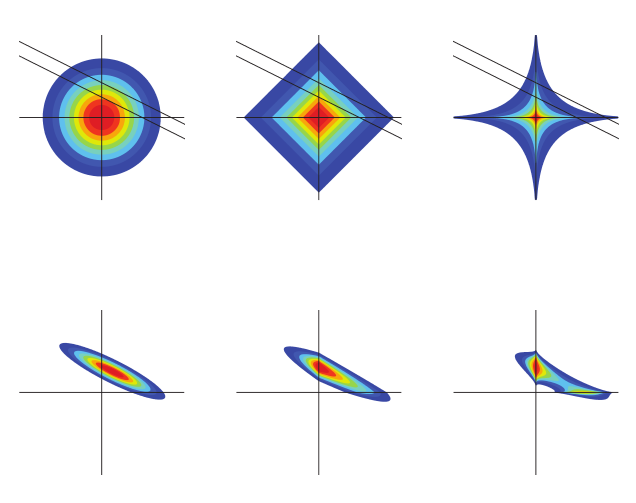
\includegraphics[width=0.7\linewidth]{fig13/figure17}
	\caption*{图13.17: 顶部:具有单位方差的三种不同分布的对数先验图:高斯、拉普拉斯和指数幂。底部:观察单个观察后的对数后验曲线图,对应于单个线性约束。该观测的精度由上图中的对角线表示。在高斯先验的情况下,后验是单峰对称的。在拉普拉斯先验的情况下,后验是单峰和不对称的(倾斜的)。在指数先验的情况下,后验是双峰的。基于(Seeger 2008)的图1。图由sparsePostPlot生成,由Florian Steinke编写。}
\end{figure}

\subsubsection*{13.6.2.1 用于HAL的EM}
由于逆伽马与拉普拉斯共轭,我们发现$\gamma_j$的E步由下式给出:
\begin{equation}
	p(\gamma_j|w_j)=IG(a+1,b+|w_j|)\tag{13.136}
\end{equation}
$\sigma^2$的E步与vanilla lasso的E步相同。

$\w$的优先权具有以下形式:
\begin{equation}
	p(\w|\gamma)=\prod_j\frac{1}{2\gamma_j}exp(-|w_j|/\gamma_j)\tag{13.137}
\end{equation}
因此,M步必须优化
\begin{equation}
	\hat{\w}^{(t+1)}=\argmax_\w \log \mathcal{N}(\y|\X\w,\sigma^2)-\sum_{j}|w_j|\mathbb{E}[1/\gamma_j]\tag{13.138}
\end{equation}

\begin{figure}[h]
	\centering
	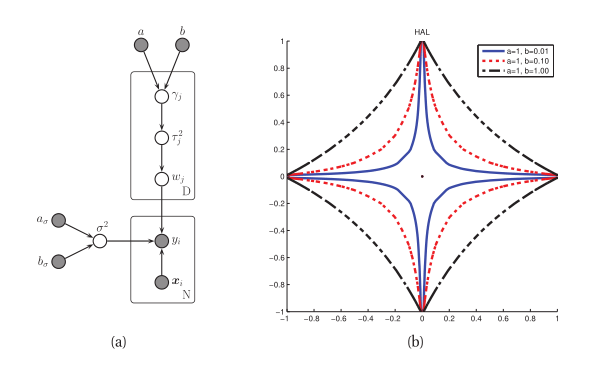
\includegraphics[width=0.7\linewidth]{fig13/figure18}
	\caption*{图13.18:(a)分层自适应lasso的DGM。(b) 层次调整拉普拉斯的轮廓。基于图1(Lee等人,2010)。图由normalGammaPenaltyPlotDemo生成。}
\end{figure}
期望值由下式给出:
\begin{equation}
	\mathbb{E}[1/\gamma_j]=\dfrac{a+1}{b+|w_j^{(t)}|}\triangleq s_j^{(t)}\tag{13.139}
\end{equation}
因此,M步成为加权lasso问题:
\begin{equation}
	\hat{\w}^{(t+1)}=\argmin_\w||\y-\X\w||_2^2+\sum_{j}s_j^{(t)}|w_j|\tag{13.140}
\end{equation}
使用标准方法(如LARS)很容易解决这一问题。请注意,如果在上一次迭代中估计系数较大(因此$w_j^{(t)}$较大),则缩放因子$s_j^{(t)}$较小,因此较大的系数不会受到严重惩罚。相反,小系数确实会受到严重惩罚。这是算法调整每个系数惩罚强度的方式。结果是一个估计值,通常比lasso返回的估计值要稀疏得多,但偏差也较小。

请注意,如果我们设置$a=b=0$,并且只执行一次EM迭代,我们得到的方法与(Zou2006;Zou和Li2008)的\textbf{自适应lasso}密切相关。该EM算法也与某些迭代重加权算法密切相关$\ell_1$信号处理界提出的方法(Chartrand和Yin,2008;Candes等人,2008)。

\subsubsection*{13.6.2.2 理解HAL的行为}
通过积分$\gamma_j$,我们可以更好地理解HAL,从而得到以下边缘分布,
\begin{equation}
	p(w_j|a,b)=\frac{a}{2b}\left(\frac{|w_j|}{b}+1\right)^{-(a+1)}\tag{13.141}
\end{equation}
\begin{figure}[h]
	\centering
	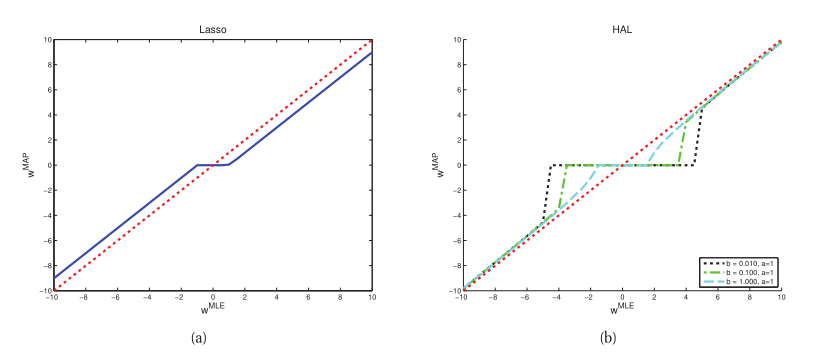
\includegraphics[width=0.7\linewidth]{fig13/figure19}
	\caption*{图13.19:两个惩罚函数的阈值行为(负对数先验)。(a) 拉普拉斯。(b)分层自适应拉普拉斯。基于图2(Lee等人,2010)。图由normalGammaThresholdPlotDemo生成。}
\end{figure}

这是\textbf{广义t分布}的一个例子(McDonald和Newey 1988)(在(Cevher 2009;Armagan等人2011)中,这被称为双帕累托分布),定义为:
\begin{equation}
	GT(w|\mu,a,c,q)\triangleq \dfrac{q}{2ca^{1/q}B(1/q,a)}\left(1+\frac{|w-\mu|^q}{ac^q}\right)^{-(a+1/q)}\tag{13.142}
\end{equation}
其中c是比例参数(控制稀疏度),a与自由度相关。当$q=2$且$c=\sqrt{2}$.恢复标准t分布;当$a\to \infty$, 我们恢复指数功率分布;当$q=1$且$a=\infty$ 我们得到拉普拉斯分布。在当前模型的上下文中,我们看到$p(w_j|a,b)=GT(w_j|0,a,b/a,1)$。

由此产生的惩罚条款具有以下形式:
\begin{equation}
	\pi_{\boldsymbol{\lambda}}(w_j)\triangleq -\log p(w_j)=(a+1)\log (1+\frac{|w_j|}{b})+const\tag{13.143}
\end{equation}
其中$\boldsymbol{\lambda}=(a,b)$是调谐参数。我们在图13.18(b)中绘制了各种b值的2d惩罚图(即,我们绘制了$\pi_{\boldsymbol{\lambda}}(w_1)+\pi_{\boldsymbol{\lambda}}(w_2)$。与图13.3(a)中所示的菱形拉普拉斯惩罚相比,我们看到HAL惩罚更像是一条“星鱼”:它沿“棘”放置了更多密度,从而更积极地强制稀疏性。请注意,此惩罚显然不是凸的。

通过考虑将该罚函数应用于具有正交设计矩阵的线性回归问题,我们可以进一步了解该罚函数的行为。在这种情况下,可以证明目标变为
\begin{align}
	J(\w)\ &=\ \frac{1}{2}||\y-\X\w||_2^2+\sum_{j=1}^{D}\pi_{\boldsymbol{\lambda}}(|w_j|)\tag{13.144}\\
	&=\ \frac{1}{2}||\y-\hat{\y}||^2+\frac{1}{2}\sum_{j=1}^{D}(\hat{w}_j^{mle}-w_j)^2+\sum_{j=1}^{D}\pi_{\boldsymbol{\lambda}}(|w_j|)\tag{13.145}
\end{align}

\begin{figure}[h]
	\centering
	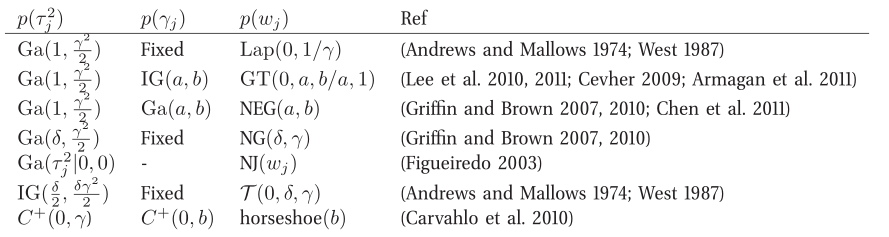
\includegraphics[width=0.7\linewidth]{fig13/table2}
	\caption*{表13.2: 高斯的一些比例混合。缩写:$C^+=$半-校正柯西;Ga$=$伽马(形状和速率参数化);GT$=$广义t;IG$=$逆伽马;NEG$=$正态指数Algamma;NG$=$正常伽马;NJ$=$正常的杰弗里斯。马蹄形分布是我们对先前描述的$w_j$上诱导的分布的名称(Carvahlo等人,2010);这没有简单的解析形式。负密度和负密度的定义有点复杂,但可以在参考文献中找到。文本中定义了其他分布。}
\end{figure}

其中$\hat{\w}^{mel}=\X^T\y$是最大似然估计,且$\hat{\y}=\X\hat{\w}^{mel}$。因此,我们可以通过解决以下1d优化问题,一次计算一维MAP估计:
\begin{equation}
	\hat{w}_j=\argmin_{w_j}\frac{1}{2}(\hat{w}_j^{mle}-w_j)^2+\pi_{\boldsymbol{\lambda}}(w_j)\tag{13.146}
\end{equation}
在图13.19(a)中,我们绘制了lasso估计值$\hat{w}^{L1}$与ML估计值,$\hat{w}^{mle}$。我们看到$\ell_1$估计器具有如图13.5(a)所示的通常软阈值行为。然而,这种行为是不可取的,因为大震级系数也向0收缩,而我们希望它们等于其unshrunken ML估计。

在图13.19(b)中,我们绘制了HAL估计值$\hat{w}^{HAL}$与ML估计值$\hat{w}^{mle}$。我们发现,这更接近图13.5(b)中所示的更理想的硬阈值行为。

\subsubsection{其他等级先验}
已经提出了许多其他等级稀疏促进先验;简要总结见表13.2。在某些情况下,我们可以解析地导出$w_j$的边际先验形式。一般来说,该先验不是凹的。

一个特别有趣的先验是不适当的正常杰弗里斯先验,它已在(Figueiredo 2003)中使用。这将非信息性Jeffreys先验置于方差$Ga(\tau_j^2|0,0)\propto1/\tau_j^2$,所得边际具有形式$p(w_j)=NJ(w_j)\propto 1/|w_j|$。这导致了阈值规则,看起来非常类似于图13.19(b)中的HAL,而这又非常类似
到硬阈值。然而,这个先验没有自由参数,这是一件好事(无需调整)和一件坏事(没有能力适应稀疏程度)。

\subsection{自动相关性确定(ARD)/稀疏贝叶斯学习(SBL)}
到目前为止,我们考虑的所有方法(第13.2.1节中的尖峰法和平板法除外)都使用了形式为$p(\w)=\prod_{j}p(w_j)$的\textbf{阶乘先验}。我们已经看到了这些先验是如何用高斯尺度$w_j\sim \mathcal{N}(0,\tau_j^2)$形式的混合来表示的,其中$\tau_j^2$具有表13.2中列出的先验之一。使用这些潜在方差,我们可以以$\tau_j^2\to w_j\to \y \gets \X$的形式表示模型,然后,我们可以使用EM进行MAP估计,在E步骤中,我们推断$p(\tau_j^2|w_j)$,在M步骤中,我们根据$\y$、$\X$和$\boldsymbol{\tau}$估计$\w$。这个M步要么涉及闭式加权$\ell_1$优化(在高斯尺度混合的情况下),或加权$\ell_1$优化(在拉普拉斯尺度混合物的情况下)。我们还讨论了如何在此类模型中执行贝叶斯推理,而不仅仅是计算MAP估计。

在本节中,我们讨论了一种基于$\mathbb{I}$型ML估计(经验贝叶斯)的替代方法,据此我们将$\w$积分并最大化边际似然wrt $\boldsymbol{\tau}$。该EB程序可以通过EM或通过重新加权$\ell_1$方案,如下所述。估计方差后,我们将其插入计算权重的后验平均值$\mathbb{E}[\w|\boldsymbol{\hat{\tau}},D]$;令人惊讶的是(考虑到高斯先验),结果是(近似)稀疏估计,原因如下所述。

在神经网络的背景下,这种方法被称为\textbf{自动相关性确定}或\textbf{ARD}(MacKay 1995b;Neal 1996):参见第16.5.7.5节。在本章中我们考虑的线性模型的背景中,这种方法称为\textbf{稀疏贝叶斯学习}或\textbf{SBL}(Tipping 2001)。将ARD/SBL与线性模型中的基函数展开相结合,产生了一种称为相关向量机(RVM)的技术,我们将在第14.3.2节中讨论。

\subsubsection{线性回归的ARD}
我们将在线性回归的背景下解释该过程;GLMs的ARD需要使用拉普拉斯(或其他)近似。在讨论ARD/SBL时,通常用$\alpha_j=1/\tau_j^2$表示权重精度,用$\beta=1/\sigma^2$表示测量精度(不要将此与统计中使用$\beta$表示回归系数混淆!)。特别是,我们将假设以下模型:
\begin{align}
	p(y|\x,\w,\beta)&=\mathcal{N}(y|w^T\x,1/\beta)\tag{13.147}\\
	p(\w)&=\mathcal{N}(\w|\0,\A^{-1})\tag{13.148}
\end{align}
其中$\A=diag(\boldsymbol{\alpha})$。边际似然可通过以下方式进行分析计算:
\begin{align}
	p(\y|\X,\boldsymbol{\alpha},\beta)&=\int \mathcal{N}(\y|\X\w,\beta\I_N)\mathcal{N}(\w|\0,\A)d\w\tag{13.149}\\
	&=\mathcal{N}(\y|\0,\beta\I_N+\X\A^{-1}\X^T)\tag{13.150}\\
	&=(2\pi)^{-N/2}|\C_\alpha|^{-\frac{1}{2}}exp(-\frac{1}{2}\y^T\C_\alpha^{-1}\y)\tag{13.151}
\end{align}
其中
\begin{equation}
	\C_{\boldsymbol{\alpha}}\triangleq \beta^{-1}\I_N+\X\A^{-1}\X^T\tag{13.152}
\end{equation}
将其与尖峰和平板模型中等式13.13中的边际似然进行比较;取第二项中缺失的$\beta=1/\sigma^2$因子的模,方程是相同的,只是我们替换了二元$\gamma_j\in \{0,1\}$具有连续的$\alpha_j\in \mathbb{R}^+$。在对数形式下,目标变为:
\begin{equation}
	\ell(\boldsymbol{\alpha},\beta)\triangleq -\frac{1}{2}\log p(\y|\X,\boldsymbol{\alpha},\beta)=\log |\C_\alpha|+\y^T\C_{\boldsymbol{\alpha}}^{-1}\y\tag{13.153}
\end{equation}

为了使问题正则化,我们可以对每个精度设置共轭先验$\alpha_j\sim Ga(a,b)$和$\beta \sim Ga(c,d)$。修改后的目标变为
\begin{align}
	\ell(\boldsymbol{\alpha},\beta)&\triangleq -\frac{1}{2}\log p(\y|\X,\boldsymbol{\alpha},\beta)+\sum_{j}\log Ga(\alpha_j|a,b)+\log Ga(\beta|c,d)\tag{13.154}\\
	&=\log |\C_\alpha|+\y^T\C_{\boldsymbol{\alpha}}^{-1}\y+\sum_{j}(a\log \alpha_j-b\alpha_j)+c\log \beta-d\beta\tag{13.155}
\end{align}
这在对$\boldsymbol{\alpha}$和$\beta$进行贝叶斯推断时非常有用(Bishop和Tipping 2000)。然而,当执行(II型)点估计时,我们将使用不适当的先验$a=b=c=d=0$,这将导致最大稀疏性。

下面我们描述如何优化$\ell(\boldsymbol{\alpha},\beta)$wrt精度项$\boldsymbol{\alpha}$和$\beta$。\footnote{优化$\beta$的另一种方法是在$\beta$上加一个伽马先验,并将其积分,得到$\w$的学生后验值(Buntine和Weigend 1991)。然而,结果表明,这导致$\boldsymbol{\alpha}$的估计不太准确(MacKay,1999)。此外,使用高斯分布比使用学生分布更容易,并且高斯情况更容易推广到其他情况,如逻辑回归。}这是在尖峰和平板模型中寻找$\boldsymbol{\gamma}$的最可能模型设置的代理,这反过来又与$\ell_0$正则化。特别是,可以证明(Wipf等人,2010年),等式13.153中的目标比$\ell_0$目标具有更少的局部最优值,因此更容易优化。

一旦我们估计了$\boldsymbol{\alpha}$和$\beta$,我们就可以使用
\begin{align}
	p(\w|D,\boldsymbol{\hat{\alpha}},\hat{\beta})&=\mathcal{N}(\boldsymbol{\mu},\boldsymbol{\textstyle \sum})\tag{13.156}\\
	\boldsymbol{\textstyle \sum}^{-1}&=\hat{\beta}\X^T\X+\A\tag{13.157}\\
	\boldsymbol{\mu}&=\hat{\beta}\boldsymbol{\textstyle \sum}\X^T\y\tag{13.158}
\end{align}
我们计算$\w$上的后验概率,同时鼓励稀疏性,这就是为什么这种方法被称为“稀疏贝叶斯学习”。然而,由于有许多方法可以实现稀疏和贝叶斯,因此我们将使用“ARD”术语,即使在线性模型上下文中也是如此。(此外,SBL只是关于系数值的“贝叶斯”,而不是反映相关变量集的不确定性,这通常更令人感兴趣。)

\begin{figure}[h]
	\centering
	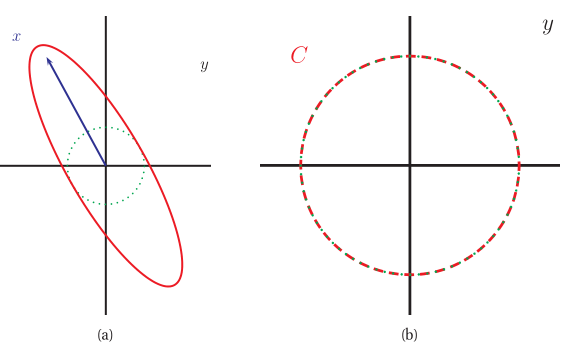
\includegraphics[width=0.7\linewidth]{fig13/figure20}
	\caption*{图13.20: 说明ARD导致稀疏性的原因。输入$\x$的矢量不指向输出$\y$的矢量,因此应删除该特征。(a) 对于有限$\alpha$,当$\alpha=\infty$, $\y$处的概率密度最大化。基于(2001年)的图8。}
\end{figure}

\subsubsection{稀疏性从何而来?}
如果$\hat{\alpha}_j\approx 0$,我们找到$\hat{w}_j\approx \hat{w}_j^{mle}$,因为高斯先验收缩$w_j$朝向0具有零精度。然而,如果我们发现$\hat{\alpha}_j\approx 0$, 那么先验知识非常确信$w_j=0$,因此特征j是“不相关的”。因此,后验平均值将具有$\hat{w}_j\approx 0$ 因此,不相关特征的权重会自动“关闭”或“删除”。

我们现在根据(Tipping 2001)给出了一个直观的论点,关于ML-II为什么应该鼓励$\alpha_j\to \infty$ 对于不相关的特征。考虑一个具有2个训练示例的一维线性回归,因此$\X=\x=(x_1,x_2)$和$\y=(y_1,y_2)$。我们可以将$\x$和$\y$绘制为平面中的向量,如图13.20所示。假设该特征与预测响应无关,因此$\x$指向与$\y$几乎正交的方向。让我们看看当我们改变$\alpha$时,边际似然会发生什么。边际似然由$p(\y|\x,\alpha,\beta)=\mathcal{N}(\y|\0,\C)$,其中
\begin{equation}
	\C=\frac{1}{\beta}\I+\frac{1}{\alpha}\x\x^T\tag{13.159}
\end{equation}
如果$\alpha$是有限的,则后部将沿x方向拉长,如图13.20(a)所示。然而,如果$\alpha=\infty$, 我们发现$\C=\frac{1}{\beta}\I$,$\C$是球形的,如图13.20(b)所示。如果$|\C|$保持不变,则后者为观测响应向量y分配更高的概率密度,因此这是首选解决方案。换句话说,边际似然“惩罚”解,其中$\alpha_j$很小,但$\X_{:,j}$不相关,因为这些浪费了概率质量。消除冗余维度更为节省(从贝叶斯-奥卡姆剃刀的角度来看)。

\subsubsection{连接到MAP估计}
ARD似乎与我们在本章前面考虑的MAP估计方法有很大不同。特别是,在ARD中,我们没有积分出$\boldsymbol{\alpha}$并优化$\w$,反之亦然。因为参数$w_j$在后验中变得相关(由于解释的原因),当我们估计$\alpha_j$时,我们借用了所有特征的信息,而不仅仅是特征j。因此,有效先验$p(\w|\boldsymbol{\hat{\alpha}})$是\textbf{非阶乘}的,而且它取决于数据$\D$(和$\sigma^2$)。然而,在(Wipf和Nagarajan,2007年)中,ARD可被视为以下MAP估计问题:

\begin{align}
	\hat{\w}^{ARD}&=\argmin_\w \beta||\y-\X\w||_2^2+g_{ARD}(\w)\tag{13.160}\\
	g_{ARD}(\w)&\triangleq \min_{\boldsymbol{\alpha}\ge 0}\sum_{j}\alpha_jw_j^2+\log |\C_{\boldsymbol{\alpha}}|\tag{13.161}
\end{align}
基于凸分析的证明有点复杂,因此省略。

此外,(Wipf和Nagarajan,2007年;Wipf等人,2010年)证明了具有非阶乘先验的MAP估计在以下意义上严格优于具有任何可能阶乘先验值的MAP估计:非阶乘目标总是比阶乘目标具有更少的局部极小值,同时仍然满足非阶乘目标的全局最优对应于$\ell_0$目标-一个属性$\ell_1$正则化没有局部极小值,因此不受欢迎。

\subsubsection{ARD算法*}
在本节中,我们将回顾几种用于实现ARD的不同算法。

\subsubsection*{13.7.4.1  EM算法}
实现SBL/ARD的最简单方法是使用EM。预期的完整数据日志可能性由下式给出:
\begin{align}
	Q(\boldsymbol{\alpha},\beta)\ &=\ \mathbb{E}[\log \mathcal{N}(\y|\X\w,\sigma^2\I)+\log \mathcal{N}(\w|\0,\A^{-1})]\tag{13.162}\\
	&=\ \frac{1}{2}\mathbb{E}\left[N\log \beta -\beta ||\y-\X\w||^2+\sum_j\log \alpha_j-tr(\A\w\w^T)\right]+const\tag{13.163}\\
	&=\ \frac{1}{2}N\log \beta -\frac{\beta}{2}(||\y-\X\boldsymbol{\mu}||^2+tr(\X^T\X\boldsymbol{\textstyle\sum}))\tag*{}\\
	&\ \ \ +\frac{1}{2}\sum_j\log \alpha_j-\frac{1}{2}tr[\A (\boldsymbol{\mu}\boldsymbol{\mu}^T+\boldsymbol{\textstyle\sum})]+const\tag{13.164}
\end{align}
其中$\boldsymbol{\mu}$和$\boldsymbol{\textstyle\sum}$在E步中使用等式13.158计算。

假设我们把$Ga(a,b)$放在$\alpha_j$上,把$Ga(c,d)$放在$\beta$上。被处罚的目标变为:
\begin{equation}
	Q'(\boldsymbol{\alpha},\beta)=Q(\boldsymbol{\alpha},\beta)+\sum_j(a\log \alpha_j-b\alpha_j)+c\log \beta-d\beta\tag{13.165}
\end{equation}
设置$\frac{dQ'}{d\alpha_j}=0$我们得到以下M步:
\begin{equation}
	\alpha_j=\dfrac{1+2a}{\mathbb{E}[w_j^2]+2b}=\dfrac{1+2a}{m_j^2+\boldsymbol{\textstyle\sum\nolimits_{jj}}+2b}\tag{13.166}
\end{equation}
如果$\alpha_j=\alpha$,$a=b=0$,则更新变为
\begin{equation}
	\alpha=\dfrac{D}{\mathbb{E}[\w^T\w]}=\dfrac{D}{\boldsymbol{\mu}^T\boldsymbol{\mu}+tr(\textstyle\sum)}\tag{13.167}
\end{equation}
$\beta$的更新由下式给出:
\begin{equation}
	\beta_{new}^{-1}=\dfrac{||\y-\X\boldsymbol{\mu}||^2+\beta^{-1}\sum_j(1-\alpha_j\textstyle\sum\nolimits_{jj})+2d}{N+2c}\tag{13.168}
\end{equation}
(这是练习13.2的推导。)

\subsubsection*{13.7.4.2  不动点算法}
一种更快更直接的方法是直接优化等式13.155中的目标。可以证明(练习13.3),等式$\frac{d\ell}{d\alpha_j}=0$和$\frac{d\ell}{d\beta}=0$导致以下定点更新:
\begin{align}
	\alpha_j\ &\gets\ \dfrac{\gamma_j+2a}{m_j^2+2b}\tag{13.169}\\
	\beta^{-1}\ &\gets\ \dfrac{||\y-\X\boldsymbol{\mu}||^2+2d}{N-\sum\nolimits_{j}\gamma_j+2c}\tag{13.170}\\
	\gamma_j\ &\triangleq\ 1-\alpha_j\sum\nolimits_{jj}\tag{13.171}
\end{align}
量$\gamma_j$是数据确定$w_j$的良好程度的量度(MacKay 1992)。因此$\gamma=\sum\nolimits_{j}\gamma_j$是模型的有效自由度。进一步讨论见第7.5.3节。

由于$\boldsymbol{\alpha}$和$\beta$都依赖于$\boldsymbol{\mu}$和$\boldsymbol{\textstyle\sum}$(可使用方程13.158或拉普拉斯近似计算),我们需要重新估计这些方程,直到收敛。(该算法的收敛性已在(Wipf和Nagarajan,2007)中进行了研究。)在收敛时,结果在形式上与EM获得的结果相同,但由于目标是非凸的,结果可能取决于初始值。

\subsubsection*{13.7.4.3  迭代重加权$\ell_1$算法}
另一种解决ARD问题的方法是基于这是一个MAP估计问题的观点。虽然对数先验$g(\w)$的形式相当复杂,但它可以被证明是$|w_j|$的非递减凹函数。这意味着它可以通过迭代重加权$\ell_1$表格问题
\begin{equation}
	\w^{t+1}=arg \min_\w NLL(\w)+\sum_{j}\lambda_j^{(t)}|w_j|\tag{13.172}
\end{equation}
在(Wipf和Nagarajan 2010)中,建议采用以下程序设置惩罚项(基于惩罚函数的凸边界)。我们用$\lambda_j^{(0)}=1$初始化,然后在迭代$t+1$时,通过迭代以下方程几次来计算$\lambda_j^{(t+1)}$:\footnote{(Wipf和Nagarajan,2007)中的算法相当于方程13.173的一次迭代。然而,由于方程计算成本低(只有$O(ND||\w^{(t+1)}||_0)$次),因此在解决更昂贵的$\ell_1$问题之前,值得迭代几次。}

\begin{equation}
	\lambda_j\gets \left[\X_{:,j}\left(\sigma^2\I+\X diag(1/\lambda_j)diag(|w_j^{(t+1)}|)\right)^{-1}\X^T)^{-1}\X_{:,j}\right]^{\frac{1}{2}}\tag{13.173}
\end{equation}
我们看到新惩罚$\lambda_j$依赖于所有旧权重。这与第13.6.2节的自适应lasso方法大不相同。

为了理解这种差异,考虑$\sigma^2=0$的无噪声情况,并假设$D\gg N$在这种情况下,存在完全重构数据的$\binom{D}{N}$解,$\X \w=\y$,并且具有稀疏性$||\w||_0=N$;这些被称为基本可行解或BFS。我们想要的是$\X\w=\y$的解,但比这个解要稀疏得多。假设该方法已找到一个BFS。我们不希望仅仅因为重量小(如自适应lasso)就增加重量的惩罚,因为这只会加强我们当前的局部最优值。相反,如果权重很小并且$||\w^{(t+1)}||<N||$,我们希望增加对权重的惩罚。协方差项($\X diag(1/\lambda_j)diag(|w_j^{(t+1)}|)^{-1}$具有这样的效果:如果$\w$是BFS,则该矩阵将是满秩的,因此惩罚不会增加太多,但如果$\w$比N稀疏,则矩阵将不会为满秩,因此与零值系数相关的惩罚将增加,从而加强了该解决方案(Wipf和Nagarajan,2010)。

\subsubsection{逻辑回归的ARD}
现在考虑二元逻辑回归,$p(y|\x,\w)=Ber(y|sigm(\w^T\x))$,使用相同的高斯先验,$p(\w)=\mathcal{N}(\w|\0,\A^{-1})$. 我们不能再使用EM来估计$\boldsymbol{\alpha}$,因为高斯先验不与logistic似然共轭,因此E步无法精确完成。一种方法是使用E步的变分近似,如第21.8.1.1节所述。更简单的方法是在E步骤中使用拉普拉斯近似(见第8.4.1节)。然后,我们可以在与之前相同的EM过程中使用此近似,但我们不再需要更新$\beta$。但是,请注意,这并不能保证收敛。

另一种方法是使用第13.7.4.3节中的技术。在这种情况下,我们可以使用精确的方法来计算内部加权$\ell_1$正则逻辑回归问题,无需近似。

\subsection{稀疏编码*}
到目前为止,我们一直专注于监督学习的稀疏先验。在本节中,我们将讨论如何将它们用于无监督学习。

在第12.6节中,我们讨论了独立分量分析,它与主成分分析类似,只是对潜在因子$\z_i$使用了非高斯先验。如果我们使非高斯先验具有稀疏性,例如拉普拉斯分布,我们将每个观察到的向量$\x_i$近似为基向量($\W$列)的稀疏组合;请注意,稀疏模式(由zi控制)随数据情况而变化。如果我们放松$\W$是正交的约束,我们就会得到一种称为\textbf{稀疏编码}的方法。在这种情况下,我们称因子加载矩阵$\W$为\textbf{字典};每列称为一个\textbf{原子}。\footnote{通常用$\D$表示字典,用$\boldsymbol{\alpha}_i$表示潜在因素。然而,我们将坚持使用$\W$和$\z_i$符号。}鉴于稀疏表示,$L>D$是常见的,在这种情况下,我们称其为\textbf{过完备}表示。

在稀疏编码中,字典可以固定或学习。如果它是固定的,则通常使用小波或DCT基,因为许多自然信号可以由少量此类基函数很好地近似。然而,通过最大化可能性,也可以学习字典
\begin{equation}
	\log p(D|\W)=\sum_{i=1}^{N}\log \int_{\z_i}\mathcal{N}(\x_i|\W\z_i,\sigma^2\I)p(\z_i)d\z_i\tag{13.174}
\end{equation}
我们将在下面讨论优化方法,然后介绍几个有趣的应用程序。

不要将稀疏编码与\textbf{稀疏PCA}混淆(参见例如(Witten等人2009;Journee等人。2010)):这将稀疏性提升先验放在回归权重$\W$上,而在稀疏编码中,我们将稀疏性提高先验放在潜在因子$\z_i$上。当然,这两种技术可以结合使用;我们称之为\textbf{稀疏矩阵分解}的结果,尽管这个术语是非标准的。有关我们的术语总结,请参见表13.3。

\subsubsection{学习稀疏编码字典}
由于等式13.174是一个难以最大化的目标,因此通常采用以下近似值:

\begin{equation}
	\log p(D|\W)\approx \sum_{i=1}^{N}\max_{\z_i}[\log \mathcal{N}(\x_i|\W\z_i,\sigma^2\I)+\log p(\z_i)]\tag{13.175}
\end{equation}
如果$p(\z_i)$是拉普拉斯,我们可以将NLL重写为
\begin{equation}
	NLL(\W,\Z)=\sum_{i=1}^{N}\frac{1}{2}||\x_i-\W\z_i||_2^2+\lambda||\z_i||_1\tag{13.176}
\end{equation}

为了防止$\W$变得任意大,通常约束$\ell_2$其列的范数小于或等于1。让我们用
\begin{equation}
	\C=\{\W\in \mathbb{R}^{D\times L}\ \ s.t.\ \ \w_j^T\w_j\le 1\}\tag{13.177}
\end{equation}
然后我们要解决$min_{\w\in c,\z\in \mathbb{R}^{N\times L}}NLL(\W,\Z)$。对于固定的$\z_i$,$\W$上的优化是一个简单的最小二乘问题。对于固定字典$\W$,$\Z$上的优化问题与lasso问题相同,存在许多快速算法。这表明了一个明显的迭代优化方案,我们在优化$\W$和$\Z$之间交替进行。(Mumford 1994)将这种方法称为\textbf{分析合成循环},其中估计基$\W$是分析阶段,估计系数$\Z$是合成阶段。在速度太慢的情况下,可以使用更复杂的算法,例如(Mairal等人,2010)。

多种其他模型导致类似于等式13.176的优化问题。例如,非负矩阵分解或NMF(Paatero和Tapper 1994;Lee和Seung 2001)需要求解形式的目标


\begin{equation}
	\min_{\w\in c,\z\in \mathbb{R}^{N\times L}}\frac{1}{2}\sum_{i=1}^{N}||\x_i-\W\z_i||_2^2\ \ \s.t. \ \ \W\ge 0,\z_i\ge 0\tag{13.178}
\end{equation}

(请注意,这没有可调整的超参数。)该约束背后的直觉是,如果学习字典是正“部分”的正和,而不是正或负的原子稀疏和,则它可能更易于解释。当然,我们可以将NMF与潜在因素的稀疏性提升先验结合起来。这称为\textbf{非负稀疏编码}(Hoyer 2004)。

或者,我们可以放弃正性约束,但对因子$\z_i$和字典$\W$施加稀疏性约束。我们称之为\textbf{稀疏矩阵分解}。为了确保严格的凸性,我们可以对权重使用弹性网类型惩罚(Mairal et al.2010),从而产生:
\begin{equation}
	\min_{\W,\Z}\frac{1}{2}\sum_{i=1}^{N}||\x_i-\W\z_i||_2^2+\lambda||\z_i||_1\ \ s.t.\  \ ||\w_j||_2^2+\gamma||\w_j||_1\le 1\tag{13.179}
\end{equation}
有几个相关的目标可以写下来。例如,我们可以用组lasso或融合lasso代替lasso NLL(Witten等人,2009)。
除了拉普拉斯,我们还可以使用其他稀疏性促进先验。例如(Zhou等人。2009)提出一种模型,其中使用第13.2.2节的二进制掩码模型使潜在因子$\z_i$稀疏。掩码的每一位都可以从具有参数$\pi $的伯努利分布中生成,该分布可以从贝塔分布中提取。或者,我们可以使用非参数先验,如beta过程。这允许模型使用大小无限的字典,而不必事先指定L。可以使用例如吉布斯采样或变分贝叶斯在该模型中执行贝叶斯推断。人们发现,由于贝叶斯奥卡姆剃刀,字典的有效大小随着噪声水平的升高而减小。这可以防止过度装配。详情见(Zhou等人,2009年)。

\subsubsection{从图像块进行字典学习的结果}
稀疏编码最近引起如此多兴趣的一个原因是它解释了神经科学中一个有趣的现象。特别是,通过对自然图像块应用稀疏编码学习的字典由基向量组成,这些基向量看起来像哺乳动物大脑初级视觉皮层中简单细胞中的滤波器(Olshausen和Field 1996)。特别是,滤波器看起来像条形和边缘检测器,如图13.21(b)所示。(在本例中,选择参数$\lambda$的目的是使主动基函数($\z_i$的非零分量)的数量约为10。)有趣的是,使用ICA可以得到视觉上类似的结果,如图13.21(a)所示。相比之下,对相同数据应用主成分分析会产生正弦光栅,如图13.21(c)所示;这些看起来不像皮质细胞反应模式。\footnote{PCA发现正弦光栅图案的原因是,它试图对数据的协方差进行建模,在图像块的情况下,协方差是平移不变的。这意味着$cov[I(x,y),I(x',y')]=f[(x-x')^2+(y-y')^2]$.对于某些函数f,其中$I(x,y)$是位置$(x,y)$处的图像强度。可以证明(Hyvarinen等人,2009年,第125页),此类矩阵的特征向量始终是不同相位的正弦曲线,即PCA发现傅里叶基。}因此,推测部分皮层可能正在执行感觉输入的稀疏编码;由此产生的潜在表征然后由更高层次的大脑进一步处理。
\begin{figure}[h]
	\centering
	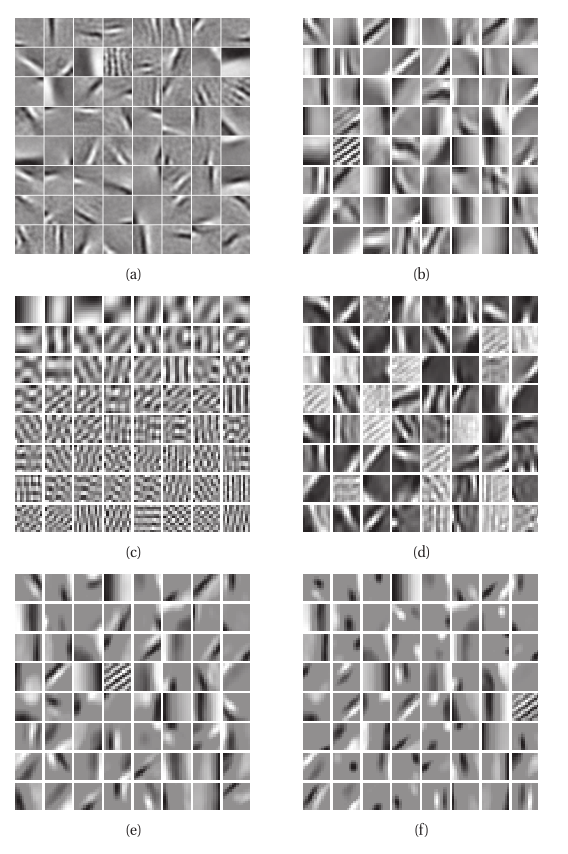
\includegraphics[width=0.7\linewidth]{fig13/figure21}
	\caption*{图13.21:当应用于自然图像块时,通过各种方法学习的滤波器示意图。(每个面片首先居中并归一化为单位范数。)(a)ICA。图由icaBasisDemo生成,由Aapo Hyvarinen提供。(b) 稀疏编码。(c) 主成分分析。(d) 非负矩阵分解。(e) 权重矩阵稀疏性低的稀疏主成分分析。(f) 权重矩阵上具有高稀疏性的稀疏PCA。图由sparseDictDemo生成,由Julien Mairal编写。}
\end{figure}

图13.21(d)显示了使用NMF的结果,图13.22(e-f)显示了稀疏PCA的结果,因为我们增加了基向量的稀疏性。

\clearpage
\subsubsection{压缩传感}
虽然通过稀疏编码学习的字典很有趣,但它不一定非常有用。然而,稀疏编码有一些实际应用,我们将在下面讨论。

想象一下,与其观察数据$x\in \mathbb{R}^D$我们观察到它的低维投影,$\y=\R\x+\boldsymbol{\epsilon}$,其中,$\y\in \mathbb{R}^M$,$\R$是$M\times D$矩阵,$M\ll D$、 然后$\epsilon$是噪声项(通常为高斯)。我们假设$\R$是一个已知的传感矩阵,对应于$\x$的不同线性投影。例如,考虑一个MRI扫描仪:每个波束方向对应一个矢量,在$\R$中编码为一行。图13.22说明了建模假设。

我们的目标是推断$p(\x|\y,\R)$。如果我们不测量所有的$\x$,我们怎么可能希望恢复所有的$\x$?答案是:我们可以使用具有适当先验的贝叶斯推理,利用自然信号可以表示为少量适当选择的基函数的加权组合这一事实。也就是说,我们假设$\x=\W\z$,其中$\z$具有稀疏先验,并且$\W$是合适的字典。这被称为压缩传感或压缩传感(Candes等人,2006年;Baruniak 2007年;Candes和Wakin 2008年;Bruckstein等人,2009年)。

对于CS来说,以正确的基础表示信号很重要,否则它将不会稀疏。在传统的CS应用程序中,字典固定为标准形式,如小波。然而,通过使用稀疏编码学习特定领域的词典,可以获得更好的性能(Zhou等人,2009)。至于传感矩阵$\R$,由于(Candes和Wakin 2008)中解释的原因,它通常被选择为随机矩阵。然而,通过将投影矩阵调整到字典中,可以获得更好的性能(Seeger和Nickish,2008;Chang等人,2009)。

\subsubsection{图像修复与去噪}
假设我们有一幅图像在某种程度上被破坏了,例如,上面稀疏地叠加了文字或划痕,如图13.23所示。我们可能需要估计底层的“干净”图像。这称为\textbf{图像修复}。可以使用类似的技术进行\textbf{图像去噪}。

\begin{figure}[h]
	\centering
	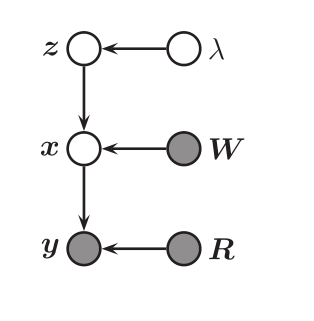
\includegraphics[width=0.7\linewidth]{fig13/figure22}
	\caption*{图13.22: 压缩传感的DGM示意图。我们观察到一个低维测量$\y$,该测量y通过测量矩阵$\R$传递$\x$生成,并且可能受到方差$\sigma^2$的观测噪声。我们假设$\x$具有字典$\W$和潜变量$\z$的稀疏分解。参数$\lambda$控制稀疏度水平。}
\end{figure}
\begin{figure}[h]
	\centering
	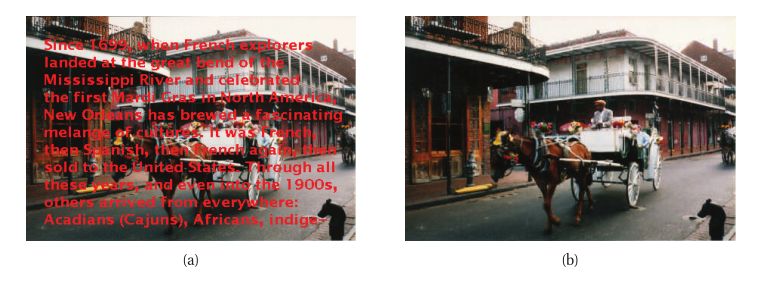
\includegraphics[width=0.7\linewidth]{fig13/figure23}
	\caption*{图13.23: 使用稀疏编码的图像修复示例。左:原始图像。右图:重建。资料来源:图13(Mairal等人,2008年)。经朱利安·迈拉尔善意许可使用。}
\end{figure}

我们可以将其建模为一种特殊的压缩感知问题。基本思想如下。我们将图像分割为重叠的面片$\y_i$,并将它们连接起来形成$\y$。我们定义$\R$,使得第i行选择面片i。现在定义$\mathcal{V}$为$\y$的可见(未损坏)分量,$\mathcal{H}$为隐藏分量。为了进行图像修复,我们只需计算$p(\y_{\mathcal{H}}|\y_{\mathcal{V}},\boldsymbol{\theta})$,其中$\boldsymbol{\theta}$是模型参数,指定字典$\W$和$\z$的稀疏度水平$\lambda$。我们可以从图像数据库离线学习字典,也可以基于未损坏的补丁为该图像学习字典。

图13.23显示了该技术的实际应用。字典(大小为256个原子)是从1200万像素图像中的$7\times 10^6$个未损坏的$12\times 12$色块中学习的。

另一种方法是使用图形模型(例如\textbf{专家领域}模型(S.and Black 2009)),该模型直接编码相邻图像块之间的相关性,而不是使用潜变量模型。不幸的是,这种模型在计算上往往更昂贵。

\subsection*{练习}

\textbf{练习13.1} RSS的偏导数

定义
\begin{equation}
	RSS(\w)=||\X\w-\y||_2^2\tag{13.180}
\end{equation}

a.证明
\begin{align}
	\frac{\partial}{\partial_{w_k}}RSS(\w)\ &=\ a_k w_k-c_k\tag{13.181}\\
	a_k\ &=\ 2\sum_{i=1}^{n}x_{ik}^2=2||x_{:,k}||^2\tag{13.182}\\
	c_k\ &=\ 2\sum_{i=1}^{n}x_{ik}(y_i-\w_{-k}^T\x_{i,-k})=2\x_{:,k}^T \r_k\tag{13.183}
\end{align}
其中$\w_{-k}=\w$,不含分量$k,\x_{i,-k}$是不含分量k的$\x_i$,并且$\r_k=\y-\w_{-k}^T\x_{:,-k}$是由于使用除特征k之外的所有特征而产生的残差。提示:将权重划分为涉及k的权重和不涉及k的权值。

b.证明,当$\frac{\partial}{\partial_{w_k}}RSS(\w)=0$,
\begin{equation}
	\hat{w}_k=\frac{\x_{:,k}^T\r_k}{||\x_{:,k}||^2}\tag{13.184}
\end{equation}

因此,当我们顺序添加特征时,特征k的最佳权重是通过计算将$\x_{:,k}$正交投影到当前残差上来计算的。

\textbf{练习13.2}线性回归EB M步的推导

推导公式13.166和13.168。提示:以下等式应该有用
\begin{align}
	\boldsymbol{\textstyle\sum}\X^T\X\ \ &=\ \ \boldsymbol{\textstyle\sum}\X^T\X+\beta^{-1}\boldsymbol{\textstyle\sum}\A-\beta^{-1}\boldsymbol{\textstyle\sum}\A\tag{13.185}\\
	&=\ \ \boldsymbol{\textstyle\sum}(\X^T\X\beta+\A)\beta^{-1}-\beta^{-1}\boldsymbol{\textstyle\sum}\A\tag{13.186}\\
	&=\ \ (\A+\beta\X^T\X)^{-1}(\X^T\X\beta+\A)\beta^{-1}-\beta^{-1}\boldsymbol{\textstyle\sum}\A\tag{13.187}\\
	&=\ \ (\I-\A\boldsymbol{\textstyle\sum})\beta^{-1}\tag{13.188}
\end{align}

\textbf{练习13.3}线性回归EB不动点更新的推导

推导方程13.169和13.170。提示:推导该结果的最简单方法是重写方程8.54中的$\log p(D|\boldsymbol{\alpha},\beta)$。这完全等价,因为在高斯先验和似然的情况下,后验也是高斯的,因此拉普拉斯“近似”是精确的。在这种情况下,我们得到

\begin{align}
	\log p(D|\boldsymbol{\alpha},\beta)=&\frac{N}{2}\log -\frac{\beta}{2}||\y-\X\w||^2\tag*{}\\
	&+\frac{1}{2}\sum_{j}\log \alpha_j-\frac{1}{2}\m^T\A\m+\frac{1}{2}\log |\boldsymbol{\textstyle\sum}|-\frac{D}{2}\log (2\pi)\tag{13.189}
\end{align}

剩下的就是简单的代数。

\textbf{练习13.4}线性回归的边际似然

假设我们使用$\boldsymbol{\textstyle\sum}_\gamma=g(\X_{\gamma}^T\X_{\gamma})^{-1}$形式的g先验.表明等式13.16简化为:

\begin{align}
	p(D|\gamma)\propto& (1+g)^{-D_\gamma/2}(2b_\sigma+S(\gamma))^{-(2a_{\sigma}+N-1)/2}\tag{13.190}\\
	S(\gamma)=& \y^T\y-\frac{g}{1+g}\y^T\X_{\gamma}(\X_{\gamma}^T\X_{\gamma})^{-1}\X_{\gamma}^T\y\tag{13.191}
\end{align}

\textbf{练习13.5}将弹性网还原为lasso

定义
\begin{equation}
	J_1(\w)=|\y-\X\w|^2+\lambda_2|\w|^2+\lambda_1|\w|_1\tag{13.192}
\end{equation}

和
\begin{equation}
	J_2(\w)=|\wty-\wtX\wtw|^2+c\lambda_1|\w|_1\tag{13.193}
\end{equation}

其中$c=(1+\lambda_2)^{-\frac{1}{2}}$,
\begin{equation}
	\boldsymbol{\wtX}=c\binom{\X}{\sqrt{\lambda_2}\I_d},\boldsymbol{\wty}=\binom{\y}{\0_{d\times 1}}\tag{13.194}
\end{equation}

证明
\begin{equation}
	arg\  min J_1(\w)=c(arg\ min J_2(\w))\tag{13.195}
\end{equation}

即
\begin{equation}
	J_1(c\w)=J_2(\w)\tag{13.196}
\end{equation}

因此,可以在修改的数据上使用lasso解算器来解决弹性网问题。

\textbf{练习13.6}线性回归中的收缩

(来源:Jaakkola。)考虑使用正交设计矩阵进行线性回归,因此,对于每列(特征)k,$||\x_{:,k}||_2^2=1$,$\x_{:,k}^T\x_{:,j}=0$,因此我们可以分别估计每个参数$w_k$。

图13.24绘制了3种不同估计方法的$\hat{w}_k$  vs $c_k=2\y^T\x_{:,k}$,特征k与响应的相关性:普通最小二乘法(OLS)、带参数$\lambda_2$的岭回归和带参数$\lambda_1$的lasso。

\begin{itemize}
\item[a.] 不幸的是,我们忘了给这些地块贴标签。实线(1)、虚线(2)和虚线(3)对应于哪种方法?提示:见第13.3.3节。
\item[b.] $\lambda_1$的值是多少?
\item[c.] $\lambda_2$的值是多少?
\end{itemize}

\textbf{练习13.7}之前,针对尖峰和平板模型中的伯努利速率参数

考虑第13.2.1节中的模型。假设我们对稀疏率$\pi_j\sim Beta(\alpha_1,\alpha_2)$。在积分$\pi_j$之后,导出$p(\boldsymbol{\gamma}|\boldsymbol{\alpha})$的表达式。讨论与固定$\pi_0$假设$\pi_j=\pi_0$相比,该方法的一些优点和缺点。

\begin{figure}[h]
	\centering
	\includegraphics[width=0.7\linewidth]{fig13/figure24}
	\caption*{图13.24: 三种不同估计器的$\hat{w}_k$与相关量$c_k$的曲线图。}
\end{figure}

\textbf{练习13.8}推导GSM之前的E步骤

证明

\begin{equation}
	\mathbb{E}\left[\frac{1}{\tau_j^2}|w_j\right]=\dfrac{\pi'(w_j)}{|w_j|}\tag{13.197}
\end{equation}

其中$\pi (w_j)=-\log p(w_j)$和$p(w_j)=int \mathcal{N}(w_j|0,\tau_j^2)p(\tau_j^2)d\tau_j^2$
提示1:

\begin{align}
	\frac{1}{\tau_j^2}\mathcal{N}(w_j|0,\tau_j^2)\ &\propto\ \frac{1}{\tau_j^2}exp(-\frac{w_j^2}{2\tau_j^2})\tag{13.198}\\
	&=\ \frac{-1}{|w_j|}\frac{-2w_j}{2\tau_j^2}exp(-\frac{w_j^2}{2\tau_j^2})\tag{13.199}\\
	&=\ \frac{-1}{|w_j|}\frac{d}{d|w_j|}\mathcal{N}(w_j|0,\tau_j^2)\tag{13.200}
\end{align}

提示2:

\begin{equation}
	\frac{d}{d|w_j|}p(w_j)=\frac{1}{p(w_j)}\frac{d}{d|w_j|}\log p(w_j)\tag{13.201}
\end{equation}

\textbf{练习13.9}拉普拉斯先验稀疏概率回归的EM

推导一种EM算法,用于使用拉普拉斯先验对权重进行二元概率分类器拟合(第9.4节)。(如果你陷入困境,请参见(Figueiredo 2003;丁和哈里森2010)

\textbf{练习13.10}组lasso的GSM表示

考虑先验$\tau_j^2\sim Ga(\delta,\rho^2/2)$,暂时忽略分组问题。由伽马混合分布在权重上产生的边际分布称为\textbf{正态伽马分布},由下式给出:

\begin{align}
	NG(w_j|\delta,\rho)\ &=\ \int \mathcal{N}(w_j|0,\tau_j^2)Ga(\tau_j^2|\delta,\rho^2/2)d\tau_j^2\tag{13.202}\\
	&=\ \frac{1}{Z}|w_j|^{\delta-1/2}\mathcal{K}_{\delta-\frac{1}{2}}(\rho|w_j|)\tag{13.203}\\
	1/Z\ &=\ \dfrac{\rho^{\delta+\frac{1}{2}}}{\sqrt{\pi}2^{\delta-1/2}\rho(\delta)}\tag{13.204}
\end{align}

其中$\mathcal{K}_{\alpha}(x)$是第二类修正贝塞尔函数(Matlab中的贝塞尔函数)。

现在假设我们有以下关于方差的先验知识:
\begin{equation}
	p(\boldsymbol{\sigma}_{1:D}^2)=\prod_{g=1}^{G}p(\boldsymbol{\sigma}_{1:d_g}^2),p(\boldsymbol{\sigma}_{1:d_g}^2)=\prod_{j\in g}Ga(\tau_j^2|\delta_g,\rho^2/2)\tag{13.205}
\end{equation}

每组权重的相应边缘具有以下形式:
\begin{equation}
	p(\w_g)\propto |u_g|^{\delta_g-d_g/2}\mathcal{K}_{\delta_g-d_g/2}(\rho u_g)\tag{13.206}
\end{equation}

其中

\begin{equation}
	u_g\triangleq\sqrt{\sum_{j\in g}w_{g,j}^2}=||\w_g||_2\tag{13.207}
\end{equation}

现在假设$\delta_g=(d_g+1)/2$,所以$\delta_g-d_g/2=\frac{1}{2}$。方便地,我们有$\mathcal{K}_{\frac{1}{2}}(z)=\sqrt{\frac{\pi}{2z}}exp(-z)$。结果表明,得到的MAP估计等价于群lasso。

\textbf{练习13.11} $\ell_1$正则化最小二乘的投影梯度下降

考虑BPDN问题$argmin_{\boldsymbol{\theta}}RSS(\boldsymbol{\theta})+\lambda||\boldsymbol{\theta}||_1$, 通过使用第7.4节中介绍的分裂变量技巧(即,通过定义$\boldsymbol{\theta}=[\boldsymbol{\theta}_+,\boldsymbol{\theta}_-]$, 将其重写为具有简单边界约束的二次规划。然后简述如何使用投影梯度下降来解决此问题。(如果你陷入困境,请咨询(Figueiredo等人,2007年)

\textbf{练习13.12}铰链损失函数的次导数

设$f(x)=(1-x)_+$是铰链损失函数,其中$(z)_+=max(0,z)$。什么是$\partial
f(0),\partial
f(1),\partial
f(2)$?

\textbf{练习13.13}凸函数的下界

设f是凸函数。解释如何在任意点$\x\in dom(f)$处找到f的全局仿射下界


\clearpage
\section{线性回归模型}

到目前为止,本书的重点一直放在无监督学习上,包括密度估计和数据聚类等主题。现在我们转向讨论监督学习,从回归开始。回归的目标是在给定$D$维\textbf{输入变量}$\mathbf{x}$的情况下预测一个或多个连续\textbf{目标变量}$t$的值。在第一章中,我们已经遇到了回归问题的一个示例,即多项式曲线拟合。多项式是一类特定的函数,属于被称为线性回归模型的广泛函数类别。这些模型共享可调参数的线性函数属性,并且将是本章的重点。最简单形式的线性回归模型也是输入变量的线性函数。然而,通过对一组固定的非线性函数(称为\textbf{基函数})进行线性组合,我们可以得到一类更加有用的函数。这些模型在参数方面是线性函数,因此具有简单的分析性质,但在输入变量方面可能是非线性的。

给定一个包含$N$个观测值$\{\mathbf{x}_n\}$的训练数据集,其中$n =1,\cdots,N$,以及相应的目标值$\{t_n\}$,目标是预测新值$\mathbf{x}$的t值。在最简单的方法中,这可以通过直接构造一个适当的函数$y(\mathbf{x})$来完成,其对新输入$\mathbf{x}$的值构成了$t$相应值的预测。更一般地,从概率的角度来看,我们的目标是建模预测分布$p(t|\mathbf{x})$,因为这表达了我们对每个$\mathbf{x}$值的$t$值的不确定性。从这个条件分布中,我们可以对任何新的值$\mathbf{x}$进行$t$的预测,以最小化适当选择的损失函数的期望值。如第1.5.5节所述,实值变量的常用损失函数是平方损失,其最优解由$t$的条件期望给出。

尽管线性模型作为模式识别的实用技术具有很大的局限性,特别是对于涉及高维输入空间的问题,但它们具有良好的分析性质,并为后面章节将要讨论的更复杂模型奠定了基础。

\subsection{线性基函数模型}

最简单的线性回归模型是指涉及输入变量线性组合的模型。

\begin{equation}
	y(\mathbf{x},\mathbf{w})=w_0+w_1x_1+\ldots+w_Dx \tag{3.1}
\end{equation}

其中$\mathbf{x}=(x_1,\ldots,x_D)^\mathrm{T}$。这通常被称为\textbf{线性回归}。该模型的关键特性是它是参数$w_0,\ldots,w_D$的线性函数。然而,它同时也是输入变量$x_i$的线性函数,这对模型施加了显著的限制。因此,我们通过考虑输入变量$x_i$的固定非线性函数的线性组合来扩展模型的类别,形式为:

\begin{equation}
	y(\mathbf{x},\mathbf{w})=w_0+\sum_{j=1}^{M-1}w_j\phi_j(\mathbf{x}) \tag{3.2}
\end{equation}

其中,$\phi_j(\mathbf{x})$被称为\textbf{基函数}。通过用$M-1$表示索引$j$ 的最大值,该模型中的参数总数将为$M$。
参数$w_0$允许数据中的存在任何固定偏移,并且有时被称为\textbf{偏置参数}(与统计意义上的“偏差”不要混淆)。通常方便定义一个额外的虚拟“基函数” $\phi_0(\mathbf{x})=1$,以便于以下形式的表示:

\begin{equation}
y(\mathbf{x},\mathbf{w})=\sum_{j=0}^{M-1}w_j\phi_j(\mathbf{x})=\mathbf{w}^{\mathrm{T}}\boldsymbol{\phi}(\mathbf{x}) \tag{3.3}
\end{equation}

其中,$\begin{aligned}\mathbf{w}=(w_0,\ldots,w_{M-1})^\mathrm{T}\end{aligned}$和$\boldsymbol{\phi}=(\phi_{0},\ldots,\phi_{M-1})^{\mathrm{T}}$。在模式识别的许多实际应用中,我们会对原始数据变量应用某种形式的固定预处理或特征提取。如果原始变量包含向量$\mathbf{x}$,则特征可以用基函数$\{\phi_{j}(\mathbf{x})\}$来表示。

通过使用非线性基函数,我们允许函数$y(\mathbf{x},\mathbf{w})$成为输入向量$\mathbf{x}$的非线性函数。式(3.2)中的函数被称为线性模型,因为该函数对$\mathbf{w}$是线性的。正是这种对参数$\mathbf{w}$的线性性质极大地简化了对这类模型的分析。然而,它也导致了一些显著的限制,正如我们在第3.6节中所讨论的那样。

第1章中考虑的多项式回归示例就是这个模型的一个特例,其中只有一个输入变量$\mathbf{x}$,并且基函数采用$\mathbf{x}$的幂次形式,即$\phi_{j}(\mathbf{x})=x^j$。多项式基函数的一个限制是它们是输入变量的全局函数,因此输入空间的一个区域的变化会影响所有其他区域。这可以通过将输入空间分割成不同的区域,并在每个区域内拟合不同的多项式来解决,从而导致样条函数(Spline functions)(Hastie et al., 2001)。

还有许多其他可能的基函数选择,例如

\begin{equation}
	\phi_j(x)=\exp\left\{-\frac{(x-\mu_j)^2}{2s^2}\right\} \tag{3.4}
\end{equation}

\begin{equation}
	\phi_j(x)=\sigma\left(\frac{x-\mu_j}s\right) \tag{3.5}
\end{equation}

\begin{equation}
	\sigma(a)=\frac1{1+\exp(-a)} \tag{3.6}
\end{equation}

\begin{equation}
	t=y(\mathbf{x},\mathbf{w})+\epsilon \tag{3.7}
\end{equation}

\begin{equation}
	p(t|\mathbf{x},\mathbf{w},\beta)=\mathcal{N}(t|y(\mathbf{x},\mathbf{w}),\beta^{-1}). \tag{3.8}
\end{equation}

\begin{equation}
	\mathbb{E}[t|\mathbf{x}]=\int tp(t|\mathbf{x})\mathrm{d}t=y(\mathbf{x},\mathbf{w}) \tag{3.9}
\end{equation}

\begin{equation}
	p(\mathbf{t}|\mathbf{X},\mathbf{w},\beta)=\prod_{n=1}^N\mathcal{N}(t_n|\mathbf{w}^\mathrm{T}\boldsymbol{\phi}(\mathbf{x}_n),\beta^{-1}) \tag{3.10}
\end{equation}

\begin{align*}
	\ln p(\mathbf{t}|\mathbf{w},\beta)\quad
	&=\sum_{n=1}^N\ln\mathcal{N}(t_n|\mathbf{w}^\mathrm{T}\boldsymbol{\phi}(\mathbf{x}_n),\beta^{-1}) \\
	&=\frac N2\ln\beta-\frac N2\ln(2\pi)-\beta E_D(\mathbf{w}) \tag{3.11}
\end{align*}

\subsubsection{最大似然和最小平方}

\subsection{偏置-方差分解}



\end{document}